%--------------------------------------------------------------
%	Trabajo Especial de Grado
%	Autor: Pedro Luis Boll Lugo
%--------------------------------------------------------------

%--------------------------------------------------------------
%	ARCHIVO PRINCIPAL
%--------------------------------------------------------------

%	Tipo de documento
\documentclass[letterpaper,12pt]{report}

%	Lista de paquetes a utilizar
\usepackage[utf8]{inputenc}
\usepackage{graphicx}
\usepackage[spanish, mexico,es-tabla]{babel}
\usepackage{url}
\usepackage{cite}
\usepackage[right=3cm,left=3cm,top=2cm,bottom=2.2cm,headsep=0.5cm,footskip=0.5cm]{geometry}
\usepackage{fancyhdr}
\usepackage{emptypage}
\usepackage[nottoc,notlot,notlof]{tocbibind}
\usepackage[justification=centering]{caption}
\usepackage[table]{xcolor}
\usepackage{color}
\usepackage{colortbl}
\usepackage{listings}
\usepackage{multicol}
\usepackage{multirow}
\usepackage{booktabs}
\usepackage{tabularx}
\usepackage{array}
\usepackage{longtable}

%	Ubicación de las imágenes 
\graphicspath{ {Figuras/} }


% 	Aquí definimos el encabezado de las paginas 
\lhead[L]{}
\chead[]{}
\rhead[]{\thepage}
\renewcommand{\headrulewidth}{0.2pt}


% 	Aquí definimos el pie de pagina de las paginas
%\lfoot[]{}
%\cfoot[]{}
%\rfoot[]{Herramienta de Automatización, Monitoreo y Análisis de Componentes y Artefactos basados en el Internet de las Cosas}
%\renewcommand{\footrulewidth}{0.2pt}

% 	Aquí definimos el encabezado y pie de pagina de la pagina inicial de un capitulo.
\fancypagestyle{plain}{
%	Encabezado
\fancyhead[L]{\rightmark}
\fancyhead[C]{}
\fancyhead[R]{\thepage}
%	Pie de pagina
%\fancyfoot[L]{}
%\fancyfoot[C]{}
%\fancyfoot[R]{Herramienta de Automatización, Monitoreo y Análisis de Componentes y Artefactos basados en el Internet de las Cosas}
\renewcommand{\headrulewidth}{0.2pt}
%\renewcommand{\footrulewidth}{0.2pt}
}
\setlength{\headheight}{16pt}

%	Estilo de las paginas (Activa encabezados y pie de pagina)
\pagestyle{fancy}


%	Tipo de referencias
\bibliographystyle{unsrt}

%	Titulo del documento
\title{Trabajo Especial de Grado}
%	Autor del documento
\author{Pedro Luis Boll Lugo}

%***************** Estructura del documento *****************

\begin{document}
%	Portada
%	Estilo de la pagina vacío
\thispagestyle{empty}

%	Forma de la pagina y centrado
\begin{minipage}[c][0.01\textheight][t]{0.85\textwidth}
\begin{center}

%	Logo de la universidad

\includegraphics[scale=0.8]{./Figuras/ucv_logo.jpg}

\bigskip\bigskip\bigskip

{\centering \scshape \large
%	Universidad 
UNIVERSIDAD CENTRAL DE VENEZUELA \\
%	Facultad
FACULTAD DE CIENCIAS \\
%	Escuela
ESCUELA DE COMPUTACIÓN \\[38pt]}


\bigskip
{\scshape \LARGE 
%	Titulo del documento
Herramienta de Automatización, Monitoreo y Análisis de Componentes y Artefactos basados en el Internet de las Cosas 
\\[60pt]} 

\vspace{5mm}

{ \scshape \renewcommand\baselinestretch{1}\selectfont    
%	Nombre y Apellido
Pedro Luis Boll Lugo\\
%	Cédula de identidad
Cédula: 20.173.376 \\[30pt]

%Tutores:
Tutor:\\
Prof. Antonio Russoniello\\[30pt]

\vspace{10mm}

%	Fecha del documento
Caracas, Octubre 2023\\[60pt]
\vfill
}


\end{center}
\end{minipage}
%   Agradecimientos
%-----------------------------------------------------------------------------
%	Resumen
%-----------------------------------------------------------------------------
\chapter*{Agradecimientos}
\addcontentsline{toc}{chapter}{Agradecimientos}
\markboth{Agradecimientos}{Agradecimientos} 
Primero agradezco a mi Dios todopoderoso, que en su infinita gloría me ha dado todo lo que he necesitado para emprender esta y todas las empresas que me he propuesto, siguiendo su plan y siendo la inspiración y participe de todas mis acciones más valiosas. Agradezco a mi familia, fuente de paz, apoyo, alegría y consuelo, especialmente a mi tía Mine, quien me inculco la profesionalidad en las cosas que hago y a mi tía Charo por sostenerme en esos detalles pequeños que la vida nos pone.\\

A mis profesores todos, quienes me han brindado su conocimiento, su experiencia y su ejemplo sin el cual llegar hasta aquí hubiese sido plenamente imposible. Especialmente agradezco a mi tutor, el profesor Antonio Russoniello por ayudarme en esta investigación de principio a fin. Para ustedes solo tengo palabras de agradecimiento y firme pensamiento de \textit{nanos gigantum humeris insidentes}.\\ 

A los Dres. Stempel quienes me ayudaron a tener todo lo que necesitaba para comenzar este Trabajo Especial de Grado. También al Dr. Rafael Apitz y a Javier Bavío por prestarme un par de artefactos para hacer dispositivos IoT y a Victor Chiaramonte quien se ofreció para hacerme un logo para la aplicación web. También a mis amigos, los de toda la vida y los que hice durante mi carrera, porque me enseñaron tanto, me soportaron, a la hora de reír y en la hora de llorar y aun así permanecen aun a mi lado.\\

A ti lector de este trabajo, por tomarte tu tiempo y querer comprender esta investigación, esperando que el conocimiento aquí depositado sea útil como lo fue para mi.\\

Por último quiero agradecer a mis padres, por ser mis ejemplos, apoyos y fuente de mi propia vida. A mi padre por ser mi mayor ejemplo de una persona trabajadora, desprendida, quien me enseñara el valor de hacer. A mi madre por enseñarme tantos valores, a ser alguien de bien. Por su amor, por su cariño, por los sacrificios que hicieron por mi y aunque ya no estén físicamente conmigo me quedo corto en las gracias por tanto. 
\vspace{35pt}
\begin{flushright}
``\textit{Los cielos cuentan la gloria de Dios y el firmamento anuncia la obra de sus manos. Un día emite palabra a otro día y una noche a otra noche declara sabiduría.}"\\
Salmos 19:1-2
\end{flushright}






% 	Resumen
%-----------------------------------------------------------------------------
%	Resumen
%-----------------------------------------------------------------------------
\chapter*{Resumen}
\addcontentsline{toc}{chapter}{Resumen}
\markboth{Resumen}{Resumen} 
En general la adopción de nuevas tecnologías suele ocurrir de manera dispar. En algunas ocasiones la adopción es lenta y paulatina lo cual permite que pueda madurar en los diversos entornos en donde se implantan así como también permite crear formas ordenadas y planificadas de crecimiento de los elementos que se encuentran involucrados. Por otro lado también existen tecnologías que debido a su rápido crecimiento hacen que las personas y organizaciones deban adaptarse y ser flexibles en la manera en que se piensa se deben usar los avances, así como también la gama completa de oportunidades y debilidades que representa su uso.\\ 

Una de esas tecnologías que ha cambiado la manera en que los seres humanos actuamos es el computador personal. Con el acceso a una plataforma tan poderosa como lo es el computador, la capacidad de poder automatizar elementos de la vida cotidiana y de procesos complejos en las industrias, se tiene la receta para ser una de las herramientas mas importantes que haya creado el hombre. Es difícil siquiera pensar en la actualidad como para incontables tareas dependemos ahora del computador. Una arista importante de dichos elementos es brindar la capacidad de computo a otros artefactos que antes no lo poseían. La arquitectura del computador moderno es lo suficientemente flexible para encontrarnos con cada vez más dispositivos que son capaces de realizar tareas aun sin la necesidad de intervención alguna.\\

Otra tecnología que ha cambiado al mundo es la capacidad de acceder y compartir información a través de una red. Su evolución a lo largo del tiempo a lo que ahora es el internet ha sido uno de los avances cruciales en la historia. No es una tecnología reciente, pero se ha masificado y democratizado su acceso de tal forma que es un aspecto omnipresente para mas de la mitad de la población mundial. Las diversas plataformas que se apoyan en la "red de redes" nos han ayudado a masificar la adopción de otro conjunto enorme de otras tecnologías, pues su flexibilidad y la madurez de los procesos que involucran la capacidad de conexión es catalizador de oportunidades para simplificar muchos aspectos de la vida hasta ahora no disponible.\\

Si juntamos los aspectos de computo y conectividad vemos que de manera disruptiva actualmente se tiene la oportunidad de mejorar y automatizar muchos de los procesos que antes por costo, logística o complejidad eran difíciles de llevar a cabo. Casi todos ahora tenemos la posibilidad de conectarnos a internet con un computador que cabe en nuestros bolsillos y poder realizar todo tipo de tareas complejas con ello. El crecimiento en la información y en masificación de artefactos y elementos que obtienen datos de su entorno proveen a los involucrados de una nueva visión del funcionamiento de las cosas es evidente cuando cada vez dichos artefactos adquieren esas capacidades de computo y conexión que antes eran impensables. A esta revolución de la información la llamamos "internet de las cosas" y es una tendencia en la tecnología en pleno crecimiento.\\ 

Sin embargo, este nuevo concepto en la manera de usar estas tecnologías no ha venido sin presentar retos y dificultades propias de cada avance. El gran volumen de información generado de manera automatizada, el control y monitoreo de dispositivos y artefactos a lo largo y ancho de complejos sistemas y y nuevos flujos automáticos donde antes no eran posibles de realizar hacen cada vez mas difícil el poder tener un panorama claro de las operaciones de estos sistemas por lo que se requieren de infraestructuras, plataformas y desarrollos nuevos para poder mejorar los aspectos de adopción mas ordenada de una forma tan nueva de hacer las cosas. Es así como nace la propuesta de comenzar a realizar la integración de tecnologías probadas que juntas puedan dar un mejor panorama en la observación y control de elementos de las operaciones y acciones que llevamos a cabo de manera automatizada en nuestro día a día.\\

El potencial que representa el internet de las cosas estará incompleto sin sistemas que sean capaces de brindar de manera adecuada información útil a los usuarios y la posibilidad de brindar la capacidad de controlar flujos automáticos de manera simple, se que este desencadene una serie de actividades en nuestro hogar o sea un complejo conjunto de operaciones criticas en una industria. A continuación se presenta una propuesta para comenzar a llenar ese vacío, mostrando el desarrollo e investigación realizado para crear una herramienta de visualización de datos de sensores de dispositivos, así como también la posibilidad de poder controlar los elementos configurables (actuadores) a través de la creación de flujos de automatización. Por tales objetivos a está software desarrollado lleva el nombre de "HAMACA" que no es más que el acronimo de "Herramienta de Automatización, Monitoreo y Análisis de Componentes y Artefactos", como tanto nos gusta a los desarrolladores usar para nombrar nuestros proyectos.\\
 
\vspace{\fill}
Palabras Claves: Internet, Computador, Internet de las Cosas, Sistemas automatizados, Monitoreo, Visualización.
\vspace{20px}
%	Indice / Tabla de Contenidos
%--------------------------------------------------------------
%	Indice de contenidos
%--------------------------------------------------------------
\tableofcontents

%--------------------------------------------------------------
%	Indice de Figuras
%--------------------------------------------------------------
\newpage
\listoffigures


%	Introducción
%-----------------------------------------------------------------------------
%	 Marco Introductorio
%-----------------------------------------------------------------------------

\lhead[\thepage]{Marco Introductorio \thechapter. \rightmark}
\rhead[Marco Introductorio \thechapter. \leftmark]{\thepage}

%	Capitulo 1: Marco Introductorio
\chapter{Introducción}
\markboth{Introducción}{Introducción}
En general la adopción de nuevas tecnologías suele ocurrir de manera dispar. En algunas ocasiones la adopción es lenta y paulatina lo cual permite que pueda madurar en los diversos entornos en donde se implantan así como también permite crear formas ordenadas y planificadas de crecimiento de los elementos que se encuentran involucrados. Por otro lado también existen tecnologías que debido a su rápido crecimiento hacen que las personas y organizaciones deban adaptarse y ser flexibles en la manera en que se piensa se deben usar los avances, así como también la gama completa de oportunidades y debilidades que representa su uso.\\ 

Una de esas tecnologías que ha cambiado la manera en que los seres humanos actuamos es el computador personal. Con el acceso a una plataforma tan poderosa, la capacidad de poder automatizar elementos de la vida cotidiana y de procesos complejos en las industrias, se tiene la receta para ser una de las herramientas más importantes que haya creado el hombre. \\

Otra tecnología que ha cambiado al mundo es la capacidad de acceder y compartir información a través de una red. Su evolución a lo largo del tiempo a lo que ahora es el Internet ha sido uno de los avances cruciales en la historia. No es una tecnología reciente, pero se ha masificado y democratizado su acceso de tal forma que es un aspecto omnipresente para mas de la mitad de la población mundial. Las diversas plataformas que se apoyan en el Internet nos han ayudado a masificar la adopción de otro conjunto enorme de otras tecnologías, pues su flexibilidad y la madurez de los procesos que involucran la capacidad de conexión es catalizador de oportunidades para resolver problemas.\\

Si juntamos los aspectos de cómputo y conectividad vemos que de manera disruptiva actualmente se tiene la oportunidad de mejorar y automatizar muchos de los procesos que antes por costo, logística o complejidad eran difíciles de llevar a cabo. El crecimiento en la información y en masificación de artefactos y elementos que obtienen datos de su entorno proveen a los involucrados de una nueva visión del funcionamiento de las cosas que no era posible. Es esta revolución de la información la llamamos ``Internet de las cosas" (también conocido en ingles como Internet of Things o IoT por sus siglas) y es una tendencia en la tecnología en pleno crecimiento y que seguirá creciendo de manera activa en los años por venir.\\ 

Sin embargo como en casi todo nuevo avance en la tecnología, no ha venido sin presentar retos y dificultades propias. El gran volumen de información generado de manera automatizada, el control y monitoreo de dispositivos y artefactos a lo largo y ancho de complejos sistemas y nuevos flujos automáticos donde antes no eran posibles de realizar hacen cada vez mas difícil el poder tener un panorama claro de las operaciones de estos sistemas por lo que se requieren de infraestructuras, plataformas y desarrollos nuevos para poder mejorar los aspectos de adopción mas ordenada de una forma tan nueva de hacer las cosas. Es así como nace la propuesta de comenzar a realizar la integración de tecnologías probadas que juntas puedan dar un mejor panorama en la observación y control de elementos de las operaciones y acciones que llevamos a cabo de manera automatizada en nuestro día a día.\\

En el siguiente trabajo de investigación se presenta una propuesta de un software que sea capaz de brindar la capacidad de mostrar datos en tiempo real e histórica provenientes de sensores y actuadores de dispositivos basados en el Internet de las cosas, así como también la capacidad de crear flujos de automatización y control de los mismos, de forma que sea una plataforma centralizada para la gestión de los dispositivos IoT dentro de un ambiente en específico.\\

En el capitulo dos presentamos de una manera detallada el problema de investigación, los antecedentes y motivaciones que llevan a examinar este problema desde el punto de vista investigativo, así como cuales son los principios que justifican indagarlo. Con ese conocimiento podemos presentar desde el punto de vista metodológico una propuesta de solución a través de un software, planteando objetivos generales y específicos dentro de un alcance que ha sido determinado bajo el contexto.\\

En los capítulos tres y cuatro se presentan los conceptos teóricos requeridos para abarcar los procesos mencionados previamente, en un primer momento tomando el concepto de Internet de las cosas de manera clara y las ventajas y desventajas que ha tenido la adopción de este tipo de tecnologías en la sociedad y luego presentando un panorama sobre las herramientas de visualización y de control existentes y como el enfoque adecuado puede ayudar a cerrar la brecha entre los datos que se van generando y las gestión de dispositivos que son cada vez mas omnipresentes como complejos.\\

Para los capítulos cinco, seis y siete presentamos el marco metodológico utilizado para diseñar, crear, probar y validar el funcionamiento integral de los componentes desarrollados con el fin de poder cumplir con los objetivos planteados, incluyendo los posibles escenarios donde este proyecto puede dar un valor agregado a las estructuras existentes.\\
 
Por último, los capítulos ocho y nueve nos dan la presentación de los resultados finales tras el desarrolló, entendiendo las circunstancias con la que se desarrollo el problema y sugiriendo una serie de trabajos futuros pueden llevarse a cabo a partir de esta base. Ademas se establecen las conclusiones a las que se llegó después de todo el trabajo realizado.

%	Capitulo uno
%-----------------------------------------------------------------------------
%	 Problema de Investigación
%-----------------------------------------------------------------------------

\lhead[\thepage]{Problema de Investigación \thechapter. \rightmark}
\rhead[Problema de Investigación \thechapter. \leftmark]{\thepage}

%	Capitulo 4: Problema de Investigación
\chapter{Problema de Investigación}
\markboth{Problema de Investigación}{Problema de Investigación}

%	Sección uno: Planteamiento del Problema
\section{Planteamiento del Problema}
\lhead[\thepage]{\thesection. Planteamiento del Problema}
El evidente incremento actual en la cantidad de dispositivos inteligentes en los últimos años ha generado que estemos rodeados de sensores de toda índole, lo que representa una oportunidades de capturar información a la cual antes no se tenia acceso. Si a esa omnipresencia le agregamos el factor de conectividad presentes en dichos dispositivos vemos que estamos ante un tipo de tecnología disruptiva con el potencial para cambiar el entorno en los que todos hacemos vida. \\

El internet de las cosas, nombre que se le da a esta combinación entre dispositivos la capacidad de conexión establece que seremos capaces de automatizar muchas más tareas complejas basándonos en microdeciciones tomadas por los mismos dispositivos, haciendo uso de la información que recolectan y actuando en consonancia con ciertos criterios, haciendo más eficientes dichos procesos, consumiendo menos recursos, alertando sobre potenciales problemas, entre otras ventajas.\\

Sin embargo la cantidad de dispositivos, el volumen de información y la capacidad de computo requerido se incrementa a pasos agigantados haciendo que la capacidad de observar cada flujo de información de procesos y el control tanto automatizado como manual de dichos dispositivos se vuelva una tarea compleja. A pesar de la existencia de múltiples herramientas que permiten palear parte de esa problemática, son pocas las opciones que cumplen tanto la función de visualización de datos, de monitorio de recursos así como también de la controlar complejos flujos de acciones de múltiples dispositivos de manera centralizada, ademas de no existir alternativas flexibles para quienes desean adaptar determinado aspecto de la automatizaciones.


\subsection{Justificación}
Dada ese situación donde es cada vez mas complejo poseer aspectos de gestión y administración de los flujos de automatización en los que se encuentran dichos dispositivos que a la larga es necesario tener a la mano una o más herramientas que permitan rescatar la observabilidad de uno de esos aspectos funcionales de las automatizaciones de procesos basados en el IoT, ya sea en el monitoreo de los sensores, en la gestión de data e información en tiempo real o histórica y por último el control de dichos dispositivos bajo rutinas predeterminadas.\\

Esto también significa que para quienes se encarguen de realizar inteligencia de negocios sobre dichos datos masivos se encuentran en una posición difícil para tratar de entender el contexto de los mismos y que información pueden aportar sin tener que ser exhaustivos o aplicando métodos complejos para tratar la información. Incluso como usuarios finales en la vida cotidiana se nos hace cada vez mas complejo observar todos los datos que se capturan de nuestros dispositivos y verlos de manera centralizada.\\

Es allí donde se requieren una nueva generación de herramientas de monitoreo, control, análisis  y con la capacidad de poder sustentar dichos complejos procesos automáticos y presentarlos de manera fácil e intuitiva a las personas.

\subsection{Alcance}
Para comenzar a subsanar esa brecha en las herramientas se propone la creación de un desarrollo que en principio contemple una forma centralizada de monitorear y controlar dispositivos IoT, contando con la capacidad de observar los datos en tiempo real e histórico de los sensores y actuadores que se registren usando uno de los múltiples protocolos abiertos de conexión y con la capacidad de presentar información simplificada acordes a las necesidades que presente el usuario final para observar dichos datos. A su vez este trabajo debe servir de framework de desarrollos futuros en el área del IoT en general.
 
\subsection{Objetivos}
\subsubsection{Objetivos Generales}
Se plantea el desarrollo de un software que permita observar y controlar dispositivos de forma transparente, intuitiva y flexible en la forma en que se presente información en tiempo real como histórica de los sensores y actuadores de dispositivos que se registren en el. Este desarrollo también debe poseer la capacidad de extender mediante módulos futuros casos de uso para implementar o extender sus capacidades iniciales a un rango mayor de dispositivos y estándares.

\subsubsection{Objetivos Específicos}
Para alcanzar el objetivo general estipulado se plantean los siguientes objetivos específicos:
\begin{itemize} 
\item Establecer la arquitectura para una solución modular adecuada para dar soporte a un sistema basado en el monitoreo/control de dispositivos IoT de manera centralizada.
\item Construir prototipos funcionales de uno o más dispositivos IoT para la captura de datos de las variables sobre los procesos que simulen de manera realista un escenario para validar el monitoreo y gestión a traves del proyecto.
\item Seleccionar y utilizar herramientas diseñadas para trabajar con estándares abiertos y que permita la integración de múltiples herramientas de diversas índole a lo largo del proyecto, para explotar de mejor forma la información obtenida de los dispositivos.
\item Utilizar e integrar herramientas de visualización de datos de forma intuitiva, así como también que permitan el control de artefactos y dispositivos.
\end{itemize}

%	Capitulo dos
%-----------------------------------------------------------------------------
%	 Internet de las Cosas
%-----------------------------------------------------------------------------

\lhead[\thepage]{Internet de las Cosas \thechapter. \rightmark}
\rhead[Internet de las Cosas \leftmark]{\thepage}

%	Capitulo 3: Internet de las Cosas
\chapter{Internet de las Cosas}
\markboth{Internet de las Cosas}{Internet de las Cosas}
\section{Definición}
\lhead[\thepage]{\thesection. Definición}
El ``Internet de las Cosas", también conocido como IoT por sus siglas en inglés es el término utilizado para designar al conjunto de artefactos y dispositivos que poseen la capacidad de conectarse entre ellos o a otras redes como el internet de forma que pueden transmitir y recibir datos e información. De manera formal no existe una definición estandarizada sobre el concepto de IoT, pues dependiendo de la organización puede considerarse el concepto desde el punto de vista desde el cual se observe el concepto, sea desde la perspectiva de las redes, desde el punto de vista de los dispositivos o bien desde el punto de vista de los sistemas automatizados.\\

La primera aparición del término fue realizada en la conferencia ``Congressional Black Caucus Foundation 15th Annual Legislative Weekend'' en Washington, D. C. en septiembre del año 1985 por parte de Peter Lewis \cite{IoTTrueHistory} en donde define que ``El Internet de las cosas, o IoT, es la integración de personas, procesos y tecnología con dispositivos y sensores conectables para permitir el monitoreo, estado, manipulación y evaluación remota de las tendencias de dichos dispositivos''\cite{IoTFirstDef}.\\

Sin embargo este concepto fue olvidado hasta el año 1999 cuando Kevin Ashton independientemente lo utilizó ilustrar el poder de conectar Etiquetas de Identificación por Radio Frecuencia (RFID) usadas en las cadenas de suministro corporativas a Internet para contar y rastrear mercancías sin la necesidad de intervención humana\cite{iotInternetSociety}.\\

Para fines prácticos, durante esta investigación se toma el concepto de original de Peter Lewis, al ser una propuesta genérica e independiente del aspecto funcional examinado. Sin embargo es importante recalcar el hecho que las Las diversas definiciones de IoT no necesariamente están en desacuerdo, sino que enfatizan diferentes aspectos de las tecnologías aplicadas sobre los dispositivos IoT desde diferentes puntos focales y casos de uso\cite{iotInternetSociety}.

\vspace{50px}

\section{Modelos de Comunicación}
\lhead[\thepage]{\thesection. Modelos de Comunicación}
Desde el punto de vista teórico, los dispositivos IoT pueden interconectarse de varias formas. Estos siguen el marco de desarrollo planteado por el estandar RFC-7452\cite{rfc7452} en el que se plantean 4 modelos de comunicación con características propias. Esos modelos son:

\subsection{Comunicación Dispositivo a Dispositivo}
Este modelo de comunicación es el mas simple de todos los paradigmas y consiste básicamente en poder conectar directamente los dispositivos independientemente del medio usado Los dispositivos se comunican usando alguno de los protocolos y estándares disponibles que sean capaces de comprender. En el ámbito del IoT esta comunicación se realiza de manera inalambrica y donde los datos o instrucciones suelen ser bastante pequeños o poco frecuentes (figura \ref{fig:d2d}). En grandes cantidades estaríamos en presencia de un modelo netamente distribuido.
\begin{figure}[htb]
\centering
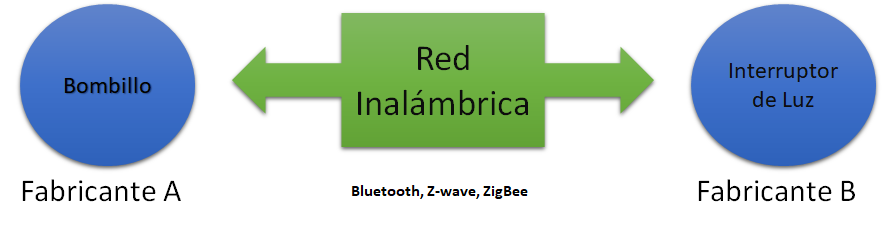
\includegraphics[scale=0.4]{./Figuras/d2d.png}
\caption{Modelo dispositivo a dispositivo}
\label{fig:d2d}
\vspace*{-10pt}
\end{figure}

  
\subsection{Comunicación Dispositivo a la Nube}
En el modelo de comunicación dispositivo a la nube, la conexión del dispositivo se conecta directamente a una nube (propia o federada) usando un proveedor de servicio (figura \ref{fig:d2n}). Este enfoque frecuentemente se aprovecha de los mecanismos de comunicación como redes celulares o la infraestructura de procesamiento de una  organización de manera directa para establecer la conexión entre el dispositivo y el servicio en la nube.
\begin{figure}[htb]
\centering
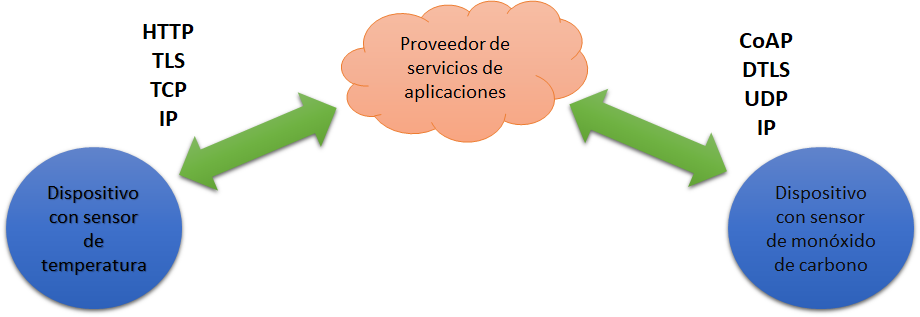
\includegraphics[scale=0.4]{./Figuras/d2n.png}
\caption{Modelo dispositivo a la nube}
\label{fig:d2n}
\vspace*{-10pt}
\end{figure}

\subsection{Comunicación Dispositivo a Puerta de Enlace}
El modelo de comunicación dispositivo a puerta de enlace establece una dispositivo o capa intermedia que concentre todas las comunicaciones (hub o broker) entre los dispositivos y de allí de ser necesario a otros fragmentos de la red o a internet (figura \ref{fig:d2g}). La ventaja de este enfoque es la capacidad de operar de manera centralizada parte de las comunicaciones de los dispositivos. Muchos protocolos están basados en el principio del paradigma de cliente-servidor por lo que este se adapta de manera natural al modelo.
\begin{figure}[htb]
\centering
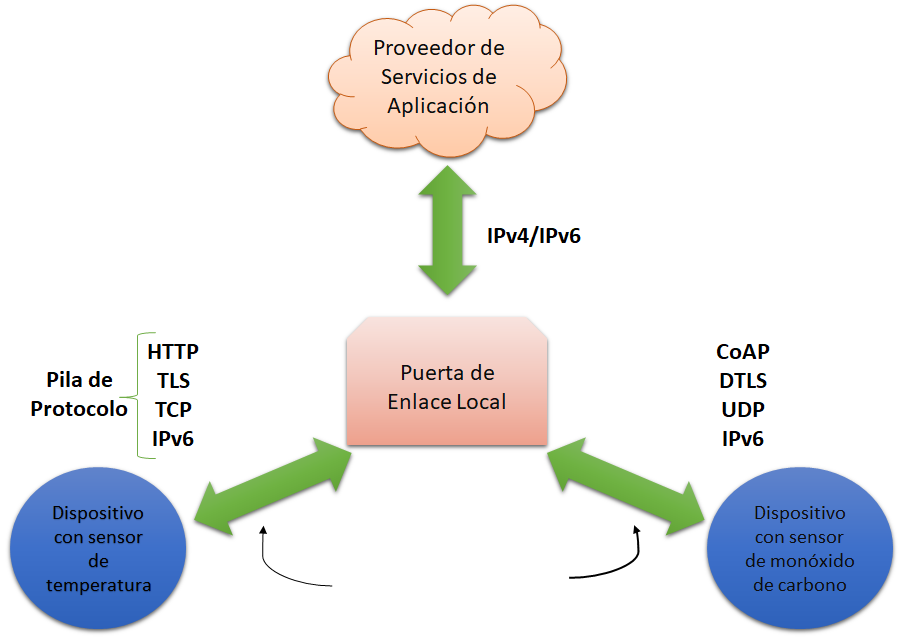
\includegraphics[scale=0.4]{./Figuras/d2g.png}
\caption{Modelo dispositivo a puerta de enlace}
\label{fig:d2g}
\vspace*{-10pt}
\end{figure}

\subsection{Comunicación Dispositivo a Intercambio de Datos en Back-end}
Este modelo es una forma automatizada de conexiones, en donde el dispositivo envía los datos a una o más APIs para de manera transparente, haciendo que este pueda intercambiar la información entre servicios que no necesariamente están estructurados o que pertenecen a un tercero (figura \ref{fig:d2b}). Particularmente este modelo es útil cuando se requiere que la información sea fácilmente accesible a través de múltiples plataformas o sistemas independientes.
\begin{figure}[htb]
\centering
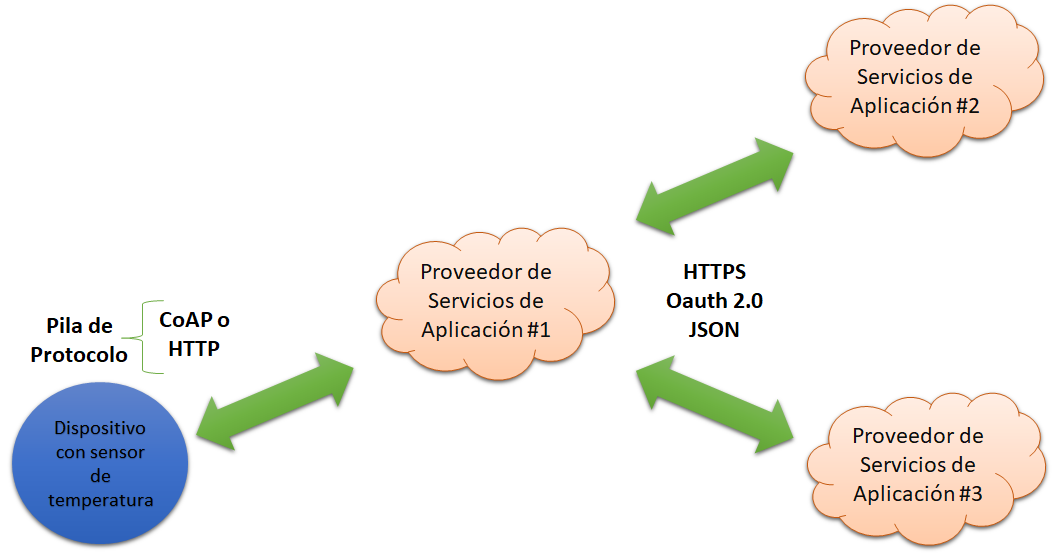
\includegraphics[scale=0.4]{./Figuras/d2b.png}
\caption{Modelo dispositivo a intercambio de datos en back-end}
\label{fig:d2b}
\vspace*{-10pt}
\end{figure}

\section{Aplicaciones del Internet de las Cosas}
\lhead[\thepage]{\thesection. Aplicaciones del Internet de las Cosas}
Si observamos la variedad de dispositivos distintos que encontramos tanto en la vida diaria como si pensamos en términos de los sistemas altamente industrializados, se hace evidente que la cantidad de distintos nichos donde el tener sensores o elementos actuadores hace que muchos procesos se vuelvan tanto dinámicos como reactivos. Las posibilidades de adopción dispositivos interconectados en flujos para automatizar procesos es algo que se está proporcionando la base de lo que llamamos computación ubicua.

Podemos categorizar según las formas de acción y su características, varios campos donde el internet de las cosas tiene y tendrá un impacto significativo para las personas y organizaciones. En la tabla \ref{tabla:categorias_dispositivos} podemos observar alguna de esas categorías y ejemplos de tecnologías acordes\cite{tablaiot}.

\begin{table}[ht]
\centering
\begin{tabular}{| m{3.2cm}| m{4.5cm}| m{6.6cm}|}
\hline
\multicolumn{3}{|c|}{Dispositivos de Internet de las Cosas} \\
\hline 
\centering Uso & \centering Descripción & \centering Ejemplos \tabularnewline \hline
Personas & Dispositivos acareados o implantados en el cuerpo humano & Dispositivos (tecnologías vestibles o digeribles) para monitorear y mantener la salud y el bienestar. Administración de tratamientos, incremento en desempeño del ejercicio físico \\ \hline
Hogar & Casas y edificios & Control de objetos y recursos del hogar y sistemas de seguridad\\ \hline
Ventas & Tiendas y distribuidores a minoristas & Tiendas, bancos, restaurantes, estadios, cualquier lugar donde un consumidor obtenga un producto o un servicio. Ofertas en tiendas, optimización de inventarios \\ \hline
Oficinas & Espacios de trabajo y de generación de conocimiento & Administración de recursos, seguridad en las oficinas. Productividad mejorada \\ \hline
Fabricas & Entornos de producción estandarizados & Lugares donde tengan rutinas repetitivas de trabajo, incluyendo granjas o lineas de producción. Operaciones eficientes, uso de equipamiento optimizado y de inventarios \\ \hline
Lugares de Construcción y extracción de material & Producción de materias primas & Infraestructuras en Minas, Petroleo y gas. Mantenimiento predictivo; seguridad laboral \\ \hline
Vehículos & Sistemas dentro de vehículos & Vehículos incluyendo carros, camiones, barcos, aviones y trenes. Mantenimiento basado en condiciones del sistema. Diseños basados en uso. Analítica preventas \\ \hline
\end{tabular}
\caption{Dispositivos de Internet de las Cosas basados en su campo de uso según McKinsey Global Institute}
\label{tabla:categorias_dispositivos}
\end{table}

\subsection{Hogares}
En los ambientes domésticos, tecnologías como el IoT son de rápida adopción. Ya podemos observar una amplia gama de distintos dispositivos que van desde bombillos inteligentes, pasando por artefactos de linea blanca hasta elementos estructurales como sensores en tuberías que permiten tener un nivel no solo de automatización sobre labores que tradicionalmente son tediosas o difíciles de realizar.\\

Las tecnologías IoT dentro de los hogares permiten tener una amplia posibilidad de personalización y comodidad, ademas que una de las promesas es que al operar obteniendo datos ambientales y de los recursos utilizados puede ajustar y optimizar su utilización lo que representa un nivel de eficiencia que antes no era posible verificar a tan alto detalle. También es posible ahora generar una serie de tareas programadas  o rutinas diarias de los habitantes, que van desde aprovechar la luz solar en las habitaciones, limpieza de robots de las habitaciones o incluso ciertos aspectos de cuidados de mascotas también son posible ahora de administrar gracias a dispositivos inteligentes.\\

Hablando del manejo y monitoreo de recursos también ahora se abre la posibilidad de atender fenómenos recurrentes o críticos. Por ejemplo, sensores en tuberías pueden determinar si el flujo y la calidad de agua es adecuado para el consumo de la vivienda, pero también determinar si existe alguna anormalidad como filtraciones. Otro caso donde puede verse uso son los sistemas de calefacción y aire acondicionados basados en termostatos inteligentes que se adaptan a la temperaturas existentes junto con otros sensores como los de movimientos dentro de una habitación para determinar la exigencia de tener una temperatura adecuada pero teniendo en cuenta el ahorro energético.\\ 

Aspectos como la seguridad también se hacen presentes en esta categoría. Los ya tradicionales sistemas de circuitos cerrados ahora son capaces de orquestarse junto con sensores de movimiento para poder determinar un escenario de intrusión o daños a la propiedad. También mediciones como los niveles de CO2 y otros gases pueden alertar a los interesados sobre condiciones potencialmente peligrosas para los habitantes, incluso con la capacidad de alertar a las autoridades sobre el hecho anormal. 

\subsection{Industrias}
Uno de los sectores con experiencia en la adopción de dispositivos con amplia variedad de sensores y actuadores son las industrias. Desde procesos roboticos cuya tolerancia sea mínima o flujos de tareas criticas para las operaciones  se han aprovechado de esto durante años. Sin embargo la llamada industria 4.0 ahora agrega el factor de la interconexión de los sistemas con los dispositivos para presentar estados e información en tiempo real de los procesos automatizados.\\

Con la información obtenida de todos sensores implicados en los procesos automatizados los gerentes pueden entender de mejor forma se debe proceder a realizar una o mas tareas, ademas de ayudar a optimizar y encontrar puntos de mejorasen  todas las etapas del proceso de producción, desde el suministro, el desarrollo y la creación, ahorrando tiempo y dinero al mismo tiempo\cite{ibmiotindustria}.\\

La retroalimentación que se va generando en las automatizaciones debido a la existencia de estos dispositivos a manera de diagnostico ayudan a poder hacer ajustes de manera inmediata en cadenas de producción y lineas de ensamblaje. Otro aspecto positivo es tener la capacidad de monitoreo y funcionamiento optimo de maquinaria, de forma de realizar mantenimientos preventivos, lo que a la larga representa una reducción de costes y una mejora en la vida útil de las herramientas. 

\subsection{Transporte}
En el caso del transporte, tanto público como privado las oportunidades que representa la capacidad de agregar sensores de manera transversal a la infraestructura existente es uno de los focos que tanto fabricantes, reguladores y gobiernos desean alcanzar. La revolución de los automóviles  con capacidades de conducción autónoma es un ejemplo claro de como los sensores son capaces de brindar los datos necesarios para la toma de decisiones de los sistemas de control del automóvil sin asistencia y esa información recolectada es también útil para entrenar modelos de inteligencia artificial que permitan elevar el nivel de autonomía en la conducción de futuros modelos\cite{ibmiottransporte1}.\\

Otro punto que se benefician es en la cadena de suministros de repuestos. Un medio de transporte que es capaz de diagnosticar anomalías hace posible que se genere una cadena de producción directa a las necesidades requeridas, desde la fabrica de la parte hasta la solicitud de chequeo por parte del usuario.\\ 
 
En los sistemas públicos de transporte se benefician de poder traducir los datos en predicciones y en alertas para los usuarios, para ajustar itinerarios y también para poder masificar los servicios a mas personas, adapatandolo a las necesidades del entorno o del momento.\\

\subsection{Comercio y Logística}
El comercio de bienes y servicios se ajusta a los modelos de intenet de las cosas al tener una observabilidad que no se tenia previamente. Desde sensores que dan estado de un producto desde su producción hasta el momento en que es adquirido y garantizan su calidad hasta datos de localización para la vigilancia de mercancías son tecnologías que ya en la actualidad se utilizan trayendo beneficio a productores como a consumidores en general, haciendo mas transparente la cadenas de producción, buscando eficiencia  y sostenibilidad como factores importantes en la actualidad.\\

Por el lado de la logística el rastreo de bienes, el intercambio de información de inventarios de manera automática basados en la identificación de productos entre proveedores, minoristas y consumidores finales genera confianza y representa nuevo niveles de seguridad, sobre todo al momento de hacer entregas de mercancías.

\subsection{Tecnologías Vestibles}
Los weareables o tecnologías vestibles es uno de esos ámbitos en donde poco a poco se esta encontrando un nicho entre las personas. Desde relojes inteligentes, lentes para realidad aumentada y realidad virtual, prendas de vestir que vigilan nuestros signos vitales, entre otros muchos ejemplos son la forma que el internet de las cosas toma forma para esta categoría. La miniaturización de sensores y de elementos de computo está haciendo posible poder crear dichos elementos y que sean cada vez mas comunes en la vida cotidiana a pesar de retos como el consumo energético de los sensores y de las comunicaciones que estos realizan\cite{ibmappsiot}.\\

Accesorios como relojes inteligentes que son capaces de leer múltiples variables fisiológicas de forma de brindar un panorama general de la salud y otras características personales o trajes especiales, utilizados sobre todo en los deportes donde se busca tener una observación mas marcada del desempeño del deportista los dispositivos ayudan a brindar una mejor perspectiva de cara a entrenamientos y de encontrar métodos para alcanzar mas rendimiento brindando métricas en tiempo real como de forma histórica.

\subsection{Medicina y Salud}
Muy a la par de las tecnologías vestibles, el área de la salud en general se ve beneficiada de la capacidad de poder obtener lecturas de variables fisiológicas así como de los signos vitales que puedan presentar los pacientes  tanto en tiempo real como a lo largo de una intervención o de un tratamiento, así poder adaptar procedimientos, medicinas, dietas de los pacientes en búsqueda de una mas rápida evolución y mejora de las personas.\\

También podemos ver un avance en la efectividad de tratamientos médicos suministrados gracias a la capacidad de obtener la información de manera mas rápida y global por la presencia de esos sensores en los dispositivos que lleven los pacientes, sumando a la tendencia de poder brindar cada vez más tratamientos personalizados \cite{ibmiotmedicina}. Ademas la conectividad del sistema de atención de la salud a través del internet de las cosas, hace hincapié en las necesidades del paciente, es decir, tratamientos proactivos, precisión mejorada cuando se trata de diagnostico, la intervención oportuna por parte del personal de salud, en miras de una medicina cada vez mas preventiva en vez de una que sea reactiva. 

\subsection{Ciudades Inteligentes}
Las ciudades en el futuro se perfilan en el uso de los dispositivos IoT como parte fundamental de la infraestructura que deben tener para brindar a sus ciudadanos la mayor cantidad de satisfacción y calidad de vida posible. Desde el punto ya tocado del transporte como el monitoreo y control de recursos vitales como es el caso del acceso a agua potable, el reciclaje de materiales, los gobiernos ya diseñan en función de la capacidad de poder contar con data de sensores para poder evaluar mejores políticas ciudadanas, así como también brindar transparencia a los procesos de gestion de recursos\cite{ibmiotciudad}. 

\section{Interoperatividad entre Infraestructuras y Dispositivos}
\lhead[\thepage]{\thesection. Interoperatividad entre Infraestructuras y Dispositivos}
Para las redes de computadoras, la interoperatividad es un elemento fundamental, incluso desde su mismo diseño, pues la idea de dispositivos conectados también requiere que se puedan comprender en un ``lenguaje" común entre las partes. Para ello existen numerosos estándares y protocolos que han surgido de forma que sean ese marco común de entendimiento entre plataformas, dispositivos y arquitecturas.\\

Más allá de los aspectos técnicos, la interoperatividad tiene una influencia significativa en el impacto económico potencial de IoT. Aquellos marcos comunes, estándares y protocolos que tienen bien definido pueden fomentar la innovación y proporcionar a los fabricantes de dispositivos IoT valor agregado gracias a esas características y a su vez, aumentar el valor económico general del mercado.\\

Además, la aplicación de las normativas y el desarrollo de nuevos estándares abiertos, cuando sea necesario, ayudan a reducir las barreras de entrada, facilitan nuevos modelos de negocio y se convierten en opciones para el usuario final así como a las organizaciones quienes las regulan o las usan. Facilita la posibilidad de elegir dispositivos con las mejores características al mejor precio e integrarlos para que trabajen juntos. Los compradores pueden ser reacios a adquirir productos y servicios IoT si hay inflexibilidad en la integración, alta complejidad de uso, la propiedad final de información obtenida o la preocupación por el bloqueo del proveedor o temor a la obsolescencia debido al cambio de los estándares\cite{iotInternetSociety}.\\

\subsection{Ecosistemas}
Los ecosistemas de dispositivos IoT no son más que la consideración planificada bajo el paraguas de uno o más estándares y/o protocolos para ofrecer características que den al usuario final un valor sobre su elección. Existen dos perspectivas sobe los ecosistemas de los dispositivos: 
\begin{itemize}
\item Ecosistemas abiertos: Generalmente creados por una organización bajo el apoyo de múltiples empresas u otras organizaciones con la idea de acordar métodos de operación que sean estandarizados a nivel de las partes interesadas. En el mundo del internet de las cosas se ve bajo la serie de tecnologías y protocolos que han sido adaptados y propuestos para poder realizar desde las tareas de comunicación, así como también en las características que sensores y actuadores envían, procesan y almacenan la información. De propósito libre y con un esquema en el cual los aportes de las comunidades y personas son escuchados tienen un ciclo de desarrollo muy rápido y una alta adopción por su flexibilidad. El principal problema que posee este enfoque es que los esfuerzos de estandarizar o el interés de organizaciones por sobre otras de utilizar las características  de un protocolo o estándar pueden dispersar los esfuerzos de adopción de fabricantes por la cantidad de posibilidades necesarias para validar un funcionamiento correcto de los dispositivos ante múltiples protocolos o estándares y el costo que conlleva. 
\item Jardines mallados: De manera contraria a los ecosistemas abiertos, los jardines mallados son desarrollados por las organizaciones para poder controlar de manera cercana la visión de los estándares y protocolos para el funcionamiento de los dispositivos. Esta visión permite que exista una integración vertical amplia y a su vez, se beneficia de un manejo muy optimo de los recursos disponibles para las tareas relacionadas. Así todos los dispositivos que están certificados para funcionar dentro de un ecosistema de estas características probablemente funcione de una manera mucho mejor de lo que lo haría en un ecosistema abierto. La contra de este enfoque es la poca flexibilidad tanto de fabricantes como de los usuarios finales para obtener características que den valor agregado a los dispositivos que desea obtener\cite{iotInternetSociety}. Ademas es común que los procesos de certificación y el coste de licenciamiento de dichos estándares y protocolos cerrados se traduzca en un precio mayor tanto para los fabricantes como para los usuarios finales.
\end{itemize}

\subsection{Riesgos}
Con respecto al tema de riesgos, podemos separarlos en dos espacios:
\begin{itemize}
\item Riesgos Programados: Los riesgos programados son aquellos riesgos que asumen los fabricantes, empresas y organizaciones al momento de diseñar, crear y ofrecer al publico un producto. En el ámbito del internet de las cosas este riesgo viene por la decisión de tomar uno o más estándares en búsqueda de interoperatividad. También se puede representar por el hecho de que se busque poner en el mercado un producto que no cumpla completamente un estándar con la probabilidad de no poder operar correctamente en un ecosistema.
\item Riesgos Técnicos: Los riesgos técnicos van presentes en las consideraciones de diseños, arquitectura y finalmente la producción de los dispositivos en si mismos. La complejidad del funcionamiento de una o más características puede verse afectada si en algunos de esas etapas existe un fallo o también por algún defecto en los componentes 
\end{itemize}

\subsection{Sistemas Heredados}
Una arista de la interoperatividad que debe considerarse en todo momento tanto como por los fabricantes, como por los usuarios finales es la capacidad de lidiar con sistemas antiguos, también llamados heredados o legados. Esto se debe a que aunque existan estándares y protocolos que son suficientemente robustos pero no están diseñados con la idea de ser extendidos hacen que dispositivos que lleven esos estándares tengan dificultades para poder cumplir con las expectativas de las industrias. Del otro lado, el tener que crear dispositivos nuevos que tengan que cumplir con estándares y protocolos desactualizados puede hacer que los costes sean mayores, así como la dificultad de brindar soporte a los mismos. 

\subsection{Configuración de dispositivos}
La configuración de dispositivos es un proceso que muchas veces es similar en aspectos como la parte de la conectividad. Sin embargo el problema se puede observar cuando la cantidad de dispositivos a configurar es alto. Esta perspectiva puede ser desalentadora para los usuarios finales quienes tienen que asumir el tiempo para hacerlo o el coste de contratación de profesionales para poder realizar todo el proceso. 

\section{Protocolos y Estándares Utilizados}
\lhead[\thepage]{\thesection. Protocolos y Estándares Utilizados}
Como se pudo observar en los puntos anteriores la existencia de estándares y de protocolos son parte fundamental para garantizar el correcto funcionamiento de cualquier dispositivo que entre dentro de cualquiera de las categorías del internet de las cosas. El lado de manejo de las redes como pilar de la tecnología requiere conocer y elegir el método adecuado de comunicarse. Es por ello que tanto los modelos planteados al principio de este capitulo\cite{rfc7452} como el protocolo adecuado puede cambiar diametralmente el desempeño del dispositivo.\\

Sin embargo, hay un valor considerable en la extensión de la capacidad de conectarse a internet a los dispositivos más restringidos en termino de recursos que a menudo necesitan versiones optimizadas o uso especial de estos protocolos. A continuación se presentan algunos de los protocolos y estándares actuales mas importantes empleados por los dispositivos del Internet de las Cosas y que han sido considerados para la investigación y el desarrollo de este trabajo.

\subsection{Protocolos}
\subsubsection{HTTP}
El protocolo de transferencia de hipertexto o mejor conocido como HTTP, es un protocolo de la capa de aplicación para la trasmisión de documentos hipermedia, como HTML. Fue diseñado para la comunicación entre los navegadores y servidores web, aunque puede ser utilizado para otros propósitos también. Sigue el patrón modelo-vista-controlador, en el que se establece una conexión, realizando una petición a un servidor y espera una respuesta del mismo. Se trata de un protocolo sin estado, lo que significa que el servidor no guarda ningún dato (estado) entre dos peticiones. Aunque la mayoría de los casos se basa en una conexión del tipo TCP /IP, pude usarse con cualquier otro protocolo del nivel de la capa de transporte orientado a conexión.\cite{mozillahttp}\\

Las principales características clave del protocolo son las siguiente:
\begin{itemize}
\item Sencillez: HTTP esta pensado y desarrollado para ser leído y fácilmente interpretado por las personas, haciendo de esta manera más fácil la depuración de errores, y reduciendo la curva de aprendizaje para las personan que empieza a trabajar con él.
\item Extensible: Presentadas en la versión HTTP/1.0, las cabeceras de HTTP, han hecho que este protocolo sea fácil de ampliar y de experimentar con él. Funcionalidades nuevas pueden desarrollarse, sin más que un cliente y su servidor, comprendan la misma semántica sobre las cabeceras de HTTP.
\item Basado en sesiones, sin estados: HTTP es un protocolo sin estado, es decir, no guarda ningún dato entre dos peticiones en la misma sesión. Esto plante la problemática, en casó de que los usuarios requieran interactuar con determinadas páginas Web, de forma ordenada y coherente. Pero mientras HTTP ciertamente es un protocolo sin estado, el uso de HTTP cookies, si permite guardar datos con respecto a la sesión de comunicación. Usando la capacidad de ampliación del protocolo HTTP, las cookies permiten crear un contexto común para cada sesión de comunicación.
\item Orientado a Conexión: Una conexión se gestiona al nivel de la capa de trasporte, y por tanto queda fuera del alcance del protocolo HTTP. Aún con este factor, HTTP no necesita que el protocolo que lo sustenta mantenga una conexión continua entre los participantes en la comunicación, solamente necesita que sea un protocolo fiable, o que no pierda mensajes (como mínimo, en todo caso, un protocolo que sea capaz de detectar que se ha pedido un mensaje y reporte un error).
\end{itemize}

HTTP es un protocolo que funciona en dos fases fundamentales, una fase de petición y una fase de respuesta. Esto se hace de la siguiente manera:

\begin{itemize}
\item En la fase de petición:
\begin{enumerate}
\item Se abre una conexión: Se utiliza un protocolo de conexión, generalmente TCP, que se usará para hacer una o una serie de peticiones y recibir una respuesta. El cliente puede abrir una conexión nueva, reusar una existente, o abrir varias a la vez hacia el servidor.
\item Se hace una petición HTTP:  Los mensajes HTTP (previos a HTTP/2) son legibles en texto plano. A partir de la versión del protocolo HTTP/2, los mensajes se encapsulan en franjas, haciendo que no sean directamente interpretables, aunque el principio de operación es el mismo.
\end{enumerate}
\item En la fase de respuesta:
\begin{enumerate}
\item Se recibe y lee la respuesta enviada por el servidor.
\item Se cierra o recicla la conexión para futuras peticiones. 
\end{enumerate}
\end{itemize}

Existen dos tipos de mensajes HTTP: peticiones y respuestas, cada uno sigue su propio formato.

\begin{itemize}
\item Petición HTTP: Consta de un método, que generalmente un verbo como GET o POST que define la operación que el cliente desea realizar, la dirección del recurso pedido en formato de URL, la versión del protocolo y el cuerpo del mensaje. Opcionalmente puede llevar cabeceras que pueden aportar mas información. 

\begin{figure}[ht]
\centering
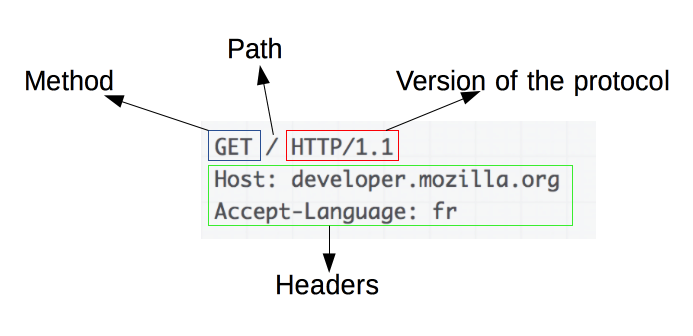
\includegraphics[width=0.625\textwidth]{Figuras/HTTP_Request.png}
\caption{\label{fig:httprequest}Formato de un mensaje de petición HTTP}
\vspace*{-15pt}
\end{figure}

\item Respuesta HTTP: Formados por los campos de versión del protocolo, el código del estado indicando si la petición fue exitosa o no y el porque, una descripción del estado, cabeceras HTTP y por ultimo y dependiendo de lo requerido, un recurso.

\begin{figure}[ht]
\centering
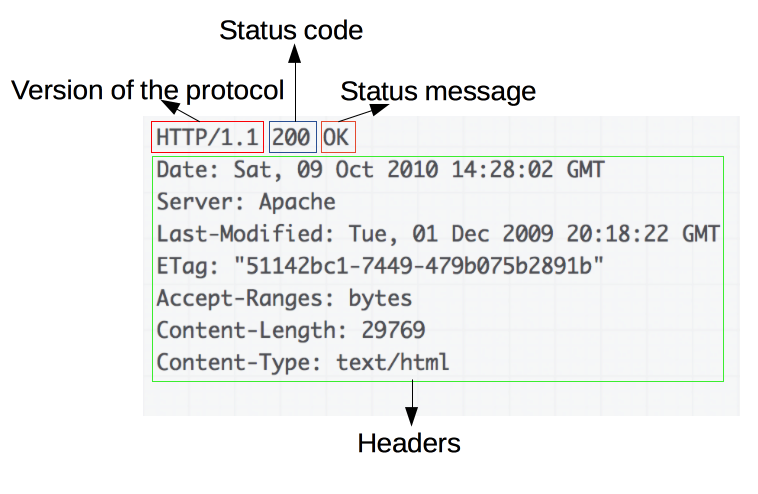
\includegraphics[width=0.5\textwidth]{Figuras/HTTP_Response.png}
\caption{\label{fig:httpresponse}Formato de un mensaje de respuesta HTTP}
\vspace*{-15pt}
\end{figure}

\end{itemize}

\subsubsection{MQTT}
MQTT son las siglas de Message Queue Telemetry Transport. Como su nombre indica, su propósito principal es la telemetría, o el monitoreo remoto. Su objetivo es recopilar datos de muchos dispositivos y transportarlos a la infraestructura de se servicios en red. Se dirige a grandes redes de pequeños dispositivos que necesitan ser monitoreados o controlados desde la nube.\cite{iotprotocols}\\

IBM creo el protocolo MQTT para poder establecer comunicación vía satélite con sensores en campos petroleros. Fue diseñado para que las comunicaciones a través de este protocolo fuesen confiables y utilizando la menor cantidad de energía posible. MQTT utiliza un modelo de publicación-suscripción y requiere un corredor MQTT central (Broker) para administrar y enrutar mensajes entre los nodos de una red MQTT. Utiliza TCP en la capa transporte, que se caracteriza por ser confiable, ordenado y con comprobación de errores.\cite{iotprocolslinkedin}\\

\begin{figure}[ht]
\centering
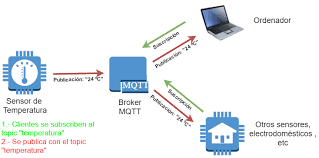
\includegraphics[width=0.85\textwidth]{./Figuras/mqtt.png}
\caption{\label{fig:mqttprotocol}Diagrama de funcionamiento del protocolo MQTT}
\vspace*{-10pt}
\end{figure}

El protocolo MQTT tiene como fortalezas:
\begin{itemize}
\item Modelo de publicación-suscripción: El modelo de publicación-suscripción es un modelo que no tiene problemas al escalar la cantidad de nodos en la red y ademas hace hace de un uso eficiente de la energía. Los Brokers y los nodos publican información y otros se suscriben según el contenido, el tipo o el tema del mensaje. (Estos son términos estándar de MQTT.) Generalmente, el Broker se suscribe a todos los mensajes y luego administra el flujo de información a sus nodos.
\item Seguridad: Al utilizar TCP como protocolo en la capa de transporte, Los paquetes MQTT no están encriptados por defecto. Pero puede utilizar la seguridad de Internet TLS/SSL. TLS es un método muy seguro para cifrar el tráfico, pero también es un recurso intensivo para clientes ligeros debido a su apretón de manos requerido y el aumento del overhead de los paquetes. Para las redes donde la energía es una prioridad muy alta y la seguridad mucho menos, cifrar sólo la carga útil del paquete puede ser suficiente.
\item Soporte para Calidad de Servicio (QoS): En MQTT, los niveles QoS 0, 1 y 2 describen niveles crecientes de entrega garantizada de mensajes. EL nivel 0 no repite paquetes, es decir, es un nivel de ``apunta y dispara". El nivel 1 intenta garantizar que un mensaje sea recibido al menos una vez por el destinatario previsto. Una vez que un mensaje publicado es recibido y comprendido por el destinatario deseado, reconoce el mensaje con un mensaje de acuse de recibo (PUBACK) dirigido al nodo de publicación. Por ultimo el nivel 2 intenta garantizar que el mensaje sea recibido y descodificado por el destinatario deseado. Este es el nivel de QoS MQTT más seguro y confiable. 
\item Testamento y ultima voluntad (LWT): MQTT proporciona un mensaje de ``último testamento" que se puede almacenar en el Broker MQTT en caso de que un nodo se desconecte inesperadamente de la red. Este LWT conserva el estado y propósito del nodo, incluyendo los tipos de comandos que publicó y sus suscripciones. Si el nodo desaparece, el intermediario notifica a todos los suscriptores del LWT del nodo. Y si el nodo vuelve, el corredor lo notifica de su estado anterior. Esta característica acomoda redes con alto porcentaje o probabilidades de  pérdidas.
\item Suscripciones flexibles de temas: Un nodo MQTT puede suscribirse a todos los mensajes dentro de una funcionalidad determinada. Por ejemplo, en un cocina un nodo horno puede suscribirse a todos los mensajes de ``cocina/horno/+", con el ``+" como comodín. Esto permite una cantidad mínima de código. Hay otros comodines MQTT igualmente útiles para reducir la cantidad del código utilizado y por lo tanto el tamaño y el coste de la memoria.
\end{itemize}

Por otro lado MQTT tiene tres desventajas evidentes:
\begin{itemize}
\item El Broker: Como intermediario central puede ser un inconveniente para los sistemas IoT distribuidos. En entornos donde la existe poca presencia de sensores y/o actuadores o donde no crece la cantidad de los dispositivos, la presencia de un Broker general latencia dentro de la red. Por otro lado el Broker puede convertirse en un único punto de fallo para la red completa.
\item El uso de TCP: TCP fue diseñado originalmente para dispositivos con más memoria y recursos de procesamiento que los que pueden estar disponibles en una red de dispositivos IoT. Por ejemplo, el protocolo TCP requiere que las conexiones se establezcan en un proceso de apretón de manos de varios pasos antes de intercambiar cualquier mensaje. Esto aumenta los tiempos de activación y de comunicación y reduce la duración de la batería a largo plazo.
\item Retrasos en la transmisión: Una vez más, el uso de TCP sin persistencia de sesión puede requerir un tiempo de transmisión incremental para el establecimiento de la conexión. Para nodos con tráfico periódico y repetitivo, esto puede afectar el consumo energético.
\end{itemize}

\begin{figure}[ht]
\centering
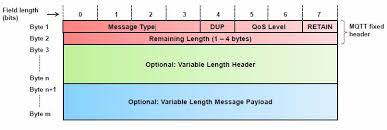
\includegraphics[width=0.9\textwidth]{./Figuras/mqtt_header.jpeg}
\caption{\label{fig:mqttheader}Formato de mensaje del protocolo MQTT}
\vspace*{-10pt}
\end{figure}


\subsubsection{IPv4 e IPv6}
Internet Protocol o IP es un protocolo de capa de red , no orientado a conexión, con una política de mejor esfuerzo en la entrega de los paquetes y cuya principal tarea es permitir la comunicación bidireccional en la red haciendo uso de direcciones a las cuales se pueden enrutar convenientemente. IP no provee ningún mecanismo para determinar si un paquete alcanza o no su destino y únicamente proporciona seguridad (mediante checksums o sumas de comprobación) de sus cabeceras y no de los datos transmitidos. \\

Este protocolo tiene como pilares fundamentales:
\begin{itemize}
\item El direccionamiento: Se refiere a la capacidad de poder asignar una dirección lógica a una interfaz de red y a su ves conocer  la manera en que se divide la red a la que pertenece.  Para el direccionamiento efectivo, el protocolo hace uso de direcciones IP, un sistema de identificación lógica y jerarquicamente una interfaz de red.
\item EL enrutamiento: el enrutamiento permite redistribuir de manera eficiente el trafico de las comunicaciones entre nodos de manera que estos puedan ir de su origen a su destino.
\end{itemize}
 
El protocolo IP en la actualidad conviven dos versiones del protocolo, IPv4 establecido en el RFC-791\cite{rfc791} e IPv6 establecida en el RFC-2460\cite{rfc2460}, ambos basados en los mismos principios pero con diferencias en la implementación.

\subsection{Estándares}
\subsubsection{Bluetooth}
Bluetooth es uno de los primeros estándares de comunicación creados pensando en dispositivos móviles. Desarrollado por la compañía sueca Ericsson estableció un protocolo de comunicación inalambrica en áreas personal, con una tasa de transmisión inicial de 1 Mbps, que luego paso a ser parte del estándar IEEE 802.15.1\cite{ieeebluetooth}. Los dispositivos Bluetooth utilizan señales de radio en la frecuencia de 2.4 GHz para establecer dicha conexión.  Con este estándar se busca que los dispositivos puedan:
\begin{itemize}
\item Establecer conexiones con poco gasto energético.
\item Establecer enlaces por lo general de corta duración.
\item Otorgar seguridad mediante diversas maneras de cifrado de datos, además de exigir el uso de un PIN para establecer conexiones entre equipos.
\item Soportar trafico de voz y datos.
\item Tener un bajo costo de producción e implementación.
\end{itemize}
En la actualidad el estándar Bluetooth se compone de un núcleo o también llamado Bluetooth Core que contiene las directivas de comunicaciones generales e inherentes al estándar y de dos extensiones llamadas Bluetooth BR/EDR (Basic Rate/Enhanced Data Rate) optimizado para hacer uso de intercambio de streams de datos, como audio y el Bluetooth Low Energy diseñado para hacer un uso muy eficiente de la energía utilizada en la comunicación, en casos donde el intercambio de datos es pequeño y que ha sido implementado desde la versión 4.0 del estándar. Los dispositivos tiene la posibilidad de implementar ya sea Bluetooth BR/EDR o Bluetooth Low Energy o ambas de forma mixta.\\

La gran ventaja de este estándar es que gran cantidad de dispositivos cuentan con la capacidad de comunicarse a través de este estándar, ademas de que permite una comunicación con un modelo dispositivo a dispositivo fácil de establecer para el usuario final. Sin embargo estas comunicaciones son de corto alcance cosa que puede afectar el desempeño entre dispositivos. El Bluetooth Low Energy abre las puertas a dispositivos que requieren manejar de manera eficiente el consumo energético de las comunicaciones pero no es aconsejado uso para el intercambio exhaustivo de información. Por otro lado, es recomendable utilizar el Bluetooth BR/EDR cuando la aplicación que se usa requiere enviar una cantidad de información importante o continuamente, pero tiene la desventaja que el consumo energético es mayor afectando negativamente la duración de los dispositivos si estos operan con una fuente estable de energía.

\subsubsection{Redes Celulares}
Los estandares celulares son las mas utilizadas en cuanto a redes inalambricas. Extendidas al rededor del mundo proveen a los dispositivos una manera sencilla de poder conectarse a servicios de voz y datos. \\

Las tecnologías de 3G son la respuesta a la especificación IMT-2000 de la Unión Internacional de Telecomunicaciones\cite{itu2000}. En Europa y Japón se seleccionó el estándar UMTS (Universal Mobile Telecommunication System)\cite{umts}, basado en la tecnología W-CDMA\cite{wcdma}. UMTS está gestionado por la organización 3GPP, también responsable de GSM, GPRS y EDGE. Para el continente americano, para África y para el resto del mundo se establecieron los estándares High-Speed Packet Access (HSPA)\cite{hspa} es una fusión de dos protocolos móviles, High Speed Downlink Packet Access (HSDPA)\cite{hspa} y High Speed Uplink Packet Access (HSUPA)\cite{hspa} que extiende y mejora el rendimiento de las redes de telecomunicaciones móviles de tercera generación (3G), como son el 3.5G o HSDPA y 3.5G Plus, 3.75G o HSUPA existentes utilizando los protocolos WCDMA.\\

La cuarta generación de tecnología en telecomunicaciones móviles, abreviado comúnmente como 4G, es el estándar aplicado al mercado móvil de la actualidad. Para que una tecnología pueda ser considerada como parte del 4G, esta debe de cumplir con ciertos requisitos para ser considerado dentro del estándar. Entre las tecnologías que se encuentran dentro de dicho estándar están: LTE-Advanced\cite{LTE-advanced}, WiMAX móvil(IEEE 802.16e)\cite{ieee80216} y WiMAX Release 2 (IEEE 802.16m).\cite{ieee80216}\\

Los requerimientos para que una red sea considerada 4G  están expuestos en la IMT-advanced de la ITU y son:
\begin{itemize}
\item Alto grado de uniformidad de funciones en todo el mundo, manteniendo al mismo tiempo la flexibilidad de admitir una amplia gama de servicios y aplicaciones rentables.
\item Compatibilidad de servicios con las IMT y las redes fijas.
\item Interoperatibilidad con otros sistemas de acceso radioeléctrico.
\item Servicios móviles con soporte para calidad de servicio.
\item Capacidad de itinerancia mundial.
\item velocidades de 100 Mbits para una movilidad alta y de 1 Gbits para una movilidad baja.
\end{itemize}

Plenamente diseñados para hacer su uso en dispositivos de carácter móvil y aprovechando la infraestructura existente, hacen de los estándares de comunicación celular una de las opciones mas fáciles y convenientes de implementar en soluciones de comunicación inalambrica, sobre todo cuando no se puede implementar una red dedicada para el trafico de los nodos. Hacen un uso eficiente de la energía del dispositivo pues los celulares y teléfonos inteligentes, pues es el recurso critico para las operaciones.

\subsubsection{NFC}
La Comunicación de Campo Cercano o NFC  por sus siglas en inglés, es un estándar que permite transferencia bidireccional de datos entre dispositivos. Su rango de transmisión es corto de máximo 10 cm de distancia, con tasas de transferencia máxima de 420kbps. El conjunto de tecnologías que permiten está comunicación están enmarcados en el estándar ISO/IEC 18000-3.\cite{isonfc}\\

NFC puede funcionar en dos modos:
\begin{itemize}
\item Activo, en el que ambos equipos con chip NFC generan un campo electromagnético e intercambian datos.
\item Pasivo, en el que solo hay un dispositivo activo y el otro aprovecha ese campo para intercambiar la información.
\end{itemize}

En cuanto a la seguridad, NFC utiliza su corta distancia de transmisión como un mecanismo de protección pues cualquier ataque deberá realizarse cerca de los dispositivos que realizan la transmisión. 

\subsubsection{Wifi (802.11)} 
WiFi es el estándar de comunicación inalambrico mas utilizado en el mundo después de las redes celulares y ha sido una selección obvia al momento de integrar comunicación dispositivos con una red. El estándar WiFI esta basado en el estadar de la IEEE 802.11\cite{ieee80211} y ha atravesado una serie de versiones que han permitido mejorar su cualidades de despliegue en termino de distancia, velocidad de transmisión, seguridad e interoperatividad.\\  

El estándar 802.11 consta de una serie de técnicas de modulación half duplex inalambrica que utilizan el mismo protocolo básico. Las versiones 802.11b y 802.11g utilizan la banda ISM de 2,4 GHz. La dificultad que representar esta banda es que los dispositivos pueden sufrir interferencias con electrodomésticos tan comunes como el microondas o el horno o con dispositivos Bluetooth. Es por que eso que deben controlar dicha susceptibilidad a las interferencias mediante métodos de señalización de espectro ensanchado por secuencia directa (DSSS) y de multiplexación por división de frecuencia ortogonal (OFDM), respectivamente.\\

Por otro lado la versión 802.11a y la versión 802.11ac utilizan la banda de 5 GHz. También hay versiones que pueden usar ambas bandas, como 802.11n pueden utilizar las bandas de 2,4 GHz o la de 5 GHz. El alcance de este estandar depende de la potencia del dispositivo, de la versión de WiFi y de las bandas utilizadas, al igual que la velocidad de transmisión pudiendo pasar de 54 Mbps a 1 Gbps. \\

A pesar de ser uno de los estándares mas utilizados, WiFI posee como inconvenientes la complejidad del hardware y software requerido así como también la cantidad de energía requerida para  establecer y mantener la comunicación, convirtiéndose en prohibitivo para dispositivos con capacidades limitadas. En las revisiones mas nuevas del estándar se esta buscando  la manera de que se mantengan las ventajas de transmisión y de espectros utilizados, sin que esto signifique un impacto severo en el consumo energético de los dispositivos. 

\subsubsection{Zigbee}
Zigbee es otro estándar de comunicación inalambrica que agrupa un conjunto de protocolos de comunicación basado en el estándar IEEE 802.15.4\cite{ieeezigbee} y que esta diseñado par a usar la banda de 2,4GHz en intercambios de paquetes poco frecuentes. Opera en un rango no mayor a 100 metros.\\

Zigbee tiene como características un funcionamiento con operación en bajo consumo energético, ofreciendo seguridad, robustez y escalabilidad de altas cantidades de nodos y dispositivos conectados y esta  pensado para ser utilizado para el intercambio de paquetes bajo un modelo dispositivo a dispositivo.\cite{iotstandars}\\

Una de las principales ventajas de Zigbee es lo sencillo y el bajo coste que supone para la empresa producir dispositivos con esta tecnología de comunicación ya que es mucho más sencillo que Bluetooth por ejemplo.\cite{androidzigbee} Existen tres distintos roles que puede cumplir un nodo o dispositivo que hace uso del estándar Zigbee:
\begin{itemize}
\item El Coordinador Zigbee: es el nodo más completo y se encarga de controlar toda la red y los caminos para su comunicación.\cite{androidzigbee} Es de carácter obligatorio para la comunicación de los los dispositivos.
\item El Router Zigbee: interconecta los nodos para poder ejecutar código del usuario, es decir, ofrece un nivel de aplicación dentro de la pila de protocolos.\cite{androidzigbee} Puede ser el mismo nodo que es Coordinador.
\item El Dispositivo: Los nodos finales de ZigBee sólo reciben información y se comunican únicamente con el nodo padre (coordinador y/o router).\cite{androidzigbee}
\end{itemize}

Zigbee es altamente utilizado en entornos industriales, sin embargo no es tan ampliamente utilizado como su rival mas cercano el estándar Bluetooth, que posee mas compañías asociadas brindadole apoyo. 

\subsubsection{Z-Wave}
El estándar Z-Wave es una tecnología de comunicación inalambrica de baja potencia diseñada principalmente para la automatización del hogar en productos como lamparas, sensores y muchos otros. Esta optimizado para ser estable, de baja latencia y con velocidad de datos de hasta 100kbps.\cite{iotstandars}\\

A diferencia de otros estándares , Z-Wave no utiliza la banda de los 2.4 GHz, sino que utiliza la banda de los 900MHz, pues con ello proporciona un rendimiento superior por dos motivos: menos interferencias (por funcionar a baja frecuencia) con otros dispositivos y mayor penetración de las ondas en paredes, pisos y muebles (al tener mayor longitud de onda).\cite{pandomzwave}\\

Una característica importante de este estándar es que  implementa redes malladas (Mesh) para la comunicación entre nodos, permitiendo una cantidad alta de dispositivos interatuando en la red y posibilitando un amplio rango en el despliegue de la misma. Los tres principales problemas que posee el estándar son:
\begin{itemize}
\item  Al utilizar un red de mallado, la comunicación entre dispositivos se maneja en cada nodo, por lo que este requiere tener un poder de procesamiento acorde para ello, ademas del gasto de energía que pueda suponer el comunicarse con múltiples puntos de la red.
\item Los chips avalados para trabajar con este estándar son fabricados por una sola compañía (Sigma Designs), lo cual afecta la producción de dispositivos  que manejen el estándar por la distribución de los chips.
\item Al usar la banda de los 900MHz dependiendo de la región en donde se planee utilizar los dispositivos, hace falta en muchos casos homologarlos pues la banda puede ser utilizada para otros propósitos.
\end{itemize}

\section{Seguridad}
\lhead[\thepage]{\thesection. Seguridad}
La seguridad de los dispositivos diseñados para formar parte del internet de las cosas, deben estar centrados no solamente en la recolección de datos, el despliegue de información o acciones sobre el ambiente sino en todos los eslabones que hagan parte del conjunto de tecnologías utilizadas para tales fines.\\

Los aspectos fundamentales de seguridad deben ser de carácter transversal a toda la infraestructura. También debe ser abordada durante todo el ciclo de vida de los dispositivos, desde el diseño inicial, pasando por las pruebas requeridas para comprobar su correcto funcionamiento, hasta la implantación en el entorno deseado y que incluye todo lo concerniente a la comunicación, al acceso y administración de los dispositivos, equipos y servicios de la arquitectura utilizada, a los datos que pueden proveer, o todo recurso que los haga un blanco ideal para los piratas informáticos.\\

Podemos separar en categorías las diferentes medidas aplicables para establecer la seguridad de la siguiente forma:

\begin{itemize}
\item Arquitecturas: Las soluciones tecnológicas deben contemplar las diversas amenazas y vulnerabilidades que puedan presentar el software, el hardware y el middleware en cada elemento de la arquitectura y que deben de ser contemplados desde la etapa de diseño. La evaluación de riesgos debe ser parte fundamental en cada escenario de uso y en cada momento de la puesta a punto de los infraestructura y validando los resultados a través del uso de pruebas, adquisición de certificados de entes competentes y reguladores y permitiendo auditorías periódicas de los resultados obtenidos.
\item Dispositivos o equipos: Para todos los equipos utilizados en los procesos en los que interviene el internet de las cosas, es importante que estos tengan durante su ciclo de vida, actualizaciones regulares que corrijan errores y malos funcionamientos, tanto a nivel del sistema operativo, firmware de dispositivos y funcionalidades previstas a nivel de software y hardware. También es importante controlar el acceso a estos dispositivos y equipos por parte de otros equipos o servicios utilizando servicios de listas blancas y listas negras.
\item Protocolos de seguridad en Internet: La seguridad que se puede brindar los protocolos de red es parte importante de las consideraciones en el diseño y funcionamiento de los dispositivos. Se establece haciendo uso de las características de encriptado, del uso de certificados de confianza y aprovechando las ventajas que pueda proveer cada protocolo en particular.  
\item Redes y Gateways: Desde el punto de vista de las redes, los dispositivos enruteadores y las puertas de enlace, la seguridad viene de la mano de los mecanismos provistos para las comunicaciones, haciendo uso de cortafuegos, logs y previniendo el acceso no autorizado a los equipos de red de manera física o remota y siempre utilizando métodos estrictos de autenticación de usuarios.
\item Protocolos de comunicación: Los protocolos de comunicación son claves para mantener a salvo la información generada y en transmisión. La clave radica en que ademas de cumplirse con los estándares de calidad y seguridad establecidos por normativas o regulaciones, también se establezcan las políticas de seguridad extras con el fin de mantener a los nodos seguros y evitando las intrusiones de terceros.
\item Consumidores y aplicaciones: Los dispositivos y equipos deben ser capaces de darle la opción a los usuarios de definir el nivel de seguridad requerido en los niveles de toda la infraestructura tecnológica utilizada, haciendo uso de interfaces de control o monitoreo. La educación de los usuarios, en cuanto a las mejores practicas y el manejo adecuado de los dispositivos, plataformas y la información generada o almacenada, es también parte fundamental para mantener la seguridad en todo momento.
\item Identificación y Privacidad: Los diversos usuarios y servicios (incluyendo las terceras partes) que pueden interactuar con los sistemas, tanto para el despliegue como para la recolección de datos e información, necesitan regirse según modelos de gestión, identificación y permisología adecuados, de manera que la privacidad, los privilegios y las integraciones y de todas las acciones que ocurren en los sistemas, estén siendo manejados de manera responsable, cumpliendo con los estándares se seguridad requeridos según el contexto.  
\end{itemize}

La acelerada proliferación y adopción de dispositivos conectados ha despertado la preocupación general por las consecuencias que podrían llegar a tener los fallos de seguridad de los mismos. Para evitar que se realicen ataques que aprovechen las vulnerabilidades de las tecnologías implicadas en el futuro hace falta realizar una serie de esfuerzos\cite{dhsiot} que ayuden a mitigar las amenazas posibles entre los cuales se sugieren:

\begin{itemize}
\item Coordinar a través de los departamentos y agencias gubernamentales para involucrarse con las partes interesadas en el aspecto de IoT y explorar conjuntamente formas de mitigar los riesgos planteados anteriormente.
\item Crear conciencia de los riesgos asociados al uso de los dispositivos entre los grupos de interés. Es importante que las partes interesadas sean conscientes de los riesgos para que puedan posicionarse y  abordarlos.
\item Identificar y promover incentivos para incorporar la seguridad. Quienes formulan políticas, los entes legisladores y las partes interesadas deben considerar formas de incentivar los esfuerzos para mejorar la seguridad de los productos. En el entorno actual, a menudo no está claro quién tiene la responsabilidad de la seguridad de un producto o sistema dado. Además, los costos de la escasa seguridad a menudo no son soportados por los que están mejor posicionados para aumentar este aspecto.  Los interesados deben considerar cómo la responsabilidad civil, la legislación, la reglamentación, la gestión voluntaria de la certificación, las iniciativas de establecimiento de normas y las iniciativas voluntarias al nivel de la industria y otros mecanismos podrían mejorar la seguridad y al mismo tiempo fomentar la actividad económica y la innovación innovadora.
\item Contribuir a los procesos de desarrollo de estándares internacionales para este ámbito. El internet de las cosas es parte de un ecosistema global, y los países y organizaciones están comenzando a evaluar muchas de estas mismas consideraciones de seguridad. Es importante que las actividades relacionadas con ello no se dividan en conjuntos inconsistentes de normas o reglas. 
\end{itemize}

%	Capitulo tres
%-----------------------------------------------------------------------------
%	 Herramientas de Monitoreo, Visualización y Control
%-----------------------------------------------------------------------------

\lhead[\thepage]{Herramientas de Monitoreo, Visualización y Control \thechapter. \rightmark}
\rhead[Herramientas de Monitoreo, Visualización y Control \thechapter. \leftmark]{\thepage}

%	Capitulo 4: Herramientas de Monitoreo, Visualización y Control
\chapter{Herramientas de Monitoreo, Visualización y Control}
\markboth{Herramientas de Visualización y Control}{Herramientas de Monitoreo, Visualización y Control}
Si el internet de las cosas es todo sobre la capacidad de conectar dispositivos con sensores y actuadores a otros dispositivos o internet para lograr uno más fines, el sentido con el que operan estos dispositivos es gracias a la generación de datos, información y de conocimiento de manera transversal a las partes implicadas. ¿Pero como podemos realmente aprovechar a los dispositivos y las ventajas que nos traen si no somos capaces de entender que datos nos proveen?.\\

A principios de este milenio, en el mundo de la tecnología se empezó a gestar uno de los paradigmas mas importantes en el área: Con los datos cada vez mas faciles de obtener, quienes fuesen capaces de interpretarlos de mejor manera y convertirlos en información útil serían quienes llevarían la punta de lanza de los nuevos desarrollos por venir. En el año 2006, Clive Humby, considerado como uno de los primeros científicos de datos, acuño la frase: ``los datos son el nuevo petroleo". Luego Micheal Palmer completo esta idea diciendo ``Los datos son  valiosos, pero si no están refinados, en realidad no se pueden usar\cite{datosPetroleo}.\\

Si examinamos detenidamente el flujo de cualquier proceso de creación de conocimiento, esta afirmación se ve respaldada plenamente. Deben existir procesos intermedios en donde estos datos se conviertan en información útil para quienes observan dichos procesos esperando responder o resolver problema, necesidad o inclusive encontrar las oportunidades que otros no han visto, ventajas que en el mundo competitivo de hoy son fundamentales. Una manera de hacer esto es a través de ordenar los datos para mostrarse basados en una lógica. Este paradigma de tratamiento de la información es natural para el ser humano, por lo que saber aprovechar de manera correcta el como presentar datos a contrapartes para respaldar una hipótesis es una forma muy efectiva de generar valor a los datos sobre un particular.\\

Ahora supongamos que los datos que observamos presentan un panorama en tiempo real de características de fenómenos y que estos de momento no persiguen actividades pasadas. El representar esos datos para hacer seguimiento del fenómeno adquiere una dimensión de vigilancia. Lamentablemente los seres humanos no son aptos para ser participe de vigilancia de datos e información a través del tiempo, pero teniendo herramientas de visualización adecuados así como ciertas rutinas establecidas según se demande en el caso caemos en el concepto de monitoreo. Esta actividad cuya faceta es en muchos aspectos pasiva puede llegar a ser tediosa por lo que contar con indicadores que ayuden a ver los cambios de estados de los fenómenos observados es vital en muchos ámbitos.\\

Pero, ¿que sucede si ese monitoreo nos remite a una situación en donde debamos actuar?, ¿como podemos cambiar las características de lo que está ocurriendo cuando muchas veces donde ocurre no es siquiera el mismo lugar geográfico donde se encuentra el fenómeno en sí? Es allí donde surgen herramientas cuyo fin es poder operar uno o múltiples flujos de tareas acordes a recetas existentes o requiriendo la intervención humana para establecer la consecución de un objetivo sobre la situación establecida. A estas herramientas las llamamos herramientas de control\\

Muchas veces encontramos herramientas que cumplen muy bien uno o incluso dos de los aspectos mencionados anteriormente. Por ejemplo, es muy común que las herramientas de visualización permitan en alguna medida el monitoreo de datos en tiempo real, o herramientas de control permitan tener la capacidad de monitorear algunos procesos de manera general.\\

La importancia de reconocer cual herramienta es la correcta para un caso u otro en particular significa que la obtención de conocimiento, la vigilancia y la gestión de procesos se realmente eficiente, aumentando el valor de las tareas que se realizan, independientemente del área al cual se aplique. A continuación se presentan de manera mas detallada las características de estas herramientas y como estos son utilizados en la actualidad en consonancia con el problema de investigación planteado.

\section{Herramientas de Visualización}
Una de las maneras en que se puede inferir un conocimiento nuevo es a través de la información que se puede desplegar de manera visual. Los seres humanos están acostumbrados a que de esta forma podamos entender mejor nuestro ambiente por lo que es natural pensar que a partir de un conjunto de datos que se presenten de manera ordenada y lógica podemos ser capaces de comprender elementos que no necesariamente se pueden ver a simple vista. Así podemos definir como la visualización de datos como la  representación gráfica de información y datos. Al utilizar elementos visuales como cuadros, gráficos y mapas\cite{visualizaciondef}.\\

Es así como el ser humano desde la antigüedad ha buscado las mejores formas de representar esos datos e información. Disciplinas como la matemática han permitido a las personas atravesar la barrera de datos inconexos a  útil y accionable. En la actualidad la gran disponibilidad de los datos hace que cada vez mas necesitemos de herramientas que no permitan resumir de forma adecuada y gráfica la descripción de uno o múltiples fenómenos de los cuales se plantea la extracción de la información. Es como las herramientas de visualización de datos proporcionan una manera accesible de ver y comprender tendencias, valores atípicos y patrones en los datos.\\

Desde el punto de vista computacional las herramientas de visualización son cada vez más importante para darle sentido a las billones de filas de datos que se generan cada día. La visualización de datos ayuda a contar historias seleccionando los datos en una forma más fácil de entender\cite{visualizaciondef} siempre recordando que el objetivo final es poder transmitir el análisis de dichos elementos a un tercero.\\

Para el caso de la investigación se ha de tener en cuenta que buscamos una forma de poder observar datos que ingresan de múltiples fuentes y características, teniendo en cuenta que los datos de los sensores de dispositivos IoT en realidad no son homogéneos y por lo tanto, los usuarios que deseen ver esos datos deben ser capaces de poder comprenderlos haciendo uso de cualquiera de los métodos existentes para visualizarlos. 

\subsection{Métodos utilizados para visualizar datos}
Independientemente de la herramientas de visualización, existen un conjunto enorme de formas de representar los datos, dependiendo de las características que estos posean. Es importante señalar el aspecto de poder seleccionar de manera correcta el método adecuado para representarlos es una elección critica, pues en una etapa de análisis, equivocarse puede representar una conclusión errónea.\\

Entre los diversos métodos de visualización tenemos:
\begin{itemize}
\item Gráficos: Las visualizaciones gráficas informan de comparaciones, relaciones y tendencias. Resaltan y hacen más claras las cifras.\cite{ibmviz} La representación gráfica permite establecer valores que no se han obtenido experimentalmente sino mediante la interpolación (lectura entre puntos) y la extrapolación (valores fuera del intervalo experimental). Entre los mas comunes tipos de gráficos están los gráficos en columnas, gráficos en barras, gráficos de linea, gráficos de área, gráficos circulares (torta o donut), entre otros.  
\item Tablas: Las tablas son formas ordenadas de datos en los cuales se busca categorizarlos basados en su posición por filas, por columnas o por ambas.
\item Mapas: Un mapa no es mas que la representación geográfica simplificada dando información relativa al plano observado.Generalmente a dos dimensiones se suelen representar las diferencias entre características usando colores.
\item Infografías: Las infografías son diagramas visuales complejos que aprovechan recursos como imágenes, texto, diagramas, logos, etc, para poder establecer de manera didáctica una idea de una manera dinámica.\
\item Cuadros de mando: Es un conjunto de indicadores representados de manera agrupada generalmente usados para representar resultados (parciales o totales) sobre datos a los que ya se las ha realizado un análisis previo. Busca representar solo la información indispensable para responder una serie de preguntas especificas.   
\end{itemize}


\section{Herramientas de Monitoreo}
Las herramientas de monitoreo son aquellas que se basan en el proceso continuo y sistemático en el cual se verifican la eficiencia y la eficacia de parámetros de uno o más elemento mediante la identificación de comportamientos o de la presentación de datos para detectar eventuales anomalías.\\

Para el proceso de monitoreo es importante entender que la vigilancia del fenómeno observado es plenamente identificable con los datos recibidos, y muchos veces estos son representados con información gráfica de manera similar a la manera que lo hacen las herramientas de visualización de datos. Sin embargo es importante entender que la visualización de datos aunque se puede dar en tiempo real, esta mas pensando para entender el pasado en base los datos mismos. El monitoreo entiende que existe previamente un conocimiento con el cual se debe regir la observación para identificar las anomalías antes mencionadas.\\

En general las herramientas de monitoreo también sirven para automatizar situaciones criticas o realizar alertas basadas en comportamientos inesperados en la data que esta ingresando. Dichas alertas pueden verse representadas en diversas formas como indicadores visuales en un panel, correos electrónicos, mensajería instantánea o cualquier otro método que este integrado y disponible para llamar la atención de los responsables e incluso permitiendo que otros sistemas puedan actuar de manera automática en respuesta a la eventualidad. 

En el marco de está investigación se requiere que la herramienta sea capaz de poder hacer el seguimiento continuo de múltiples variables sobre sensores y actuadores registrados. Esta información puede ser usada para crear alertas automáticas basadas en los patrones reconocidos anteriormente en el contexto de del dispositivo IoT. 


\section{Herramientas de Control}
Las herramientas de control difieren de las herramientas anteriores porque estos no buscan mostrar datos e información al usuario final, sino que buscan establecer formas de gestión de procesos y modificar basado en una o una serie de reglas el comportamiento de otro artefacto. Estas herramientas permiten planificar tareas y procedimientos de manera previa para un escenario dado, así como también permiten que las personas intervengan en escenarios donde se requiere del conocimiento experto no programado de una automatización.\\

En particular los software de control son todos aquellos sistemas o programas que se encuentras desplegados a lo largo o ancho de las operaciones de un flujo de trabajo y son omnipresentes en la actualidad de cualquier industria o empresa y buscan la menor intervención posible de las personas para evitar introducir el componente del error humano, así como también orquestar las acciones de procesos tediosos o costosos en recursos.\\

Una herramienta de control robusta debe ser capaz no solo llevar los procesos como fueron establecidos y automatizados sino también dar la oportunidad a los usuarios finales de tomar el mando en cualquier momento y en el mejor de los escenarios, ser lo suficientemente flexible para poder generar nuevos flujos o modificar los existentes de manera que todo el proceso sea parametrizable.\\ 

Finalmente, para el caso de los dispositivos IoT una herramienta de control debe soportar estándares y protocolos con los cuales este garantizada la interoperatividad de los sensores y actuadores, de forma que estos sean capaces de recibir ordenes de una forma centralizada acorde a las necesidades del usuario. También el fin de poder controlar los dispositivos es también generar procesos automatizados complejos a partir de programación que no necesariamente existe como regla de negocio dentro del dispositivo sino que se pueda dar a partir de los requerimientos de un usuario final.  

%	Capitulo cuatro
%-----------------------------------------------------------------------------
%	 Placas Programables
%-----------------------------------------------------------------------------

\lhead[\thepage]{Placas Programables \thechapter. \rightmark}
\rhead[Placas Programables \thechapter. \leftmark]{\thepage}

%	Capitulo 5: Placas Programables
\chapter{Placas Programables}
\markboth{Placas Programables}{Placas Programables}

%	Sección uno: Definición
\section{Definición}
\lhead[\thepage]{\thesection. Definición}
Las placas programables, también llamadas placas de programación o desarrollo son dispositivos básicos que cuentan con un microcontrolador programable con el cual se pueden ejecutar diferentes instrucciones. En muchos escenarios estamos en presencia de una computadora de recursos muy reducidos (conocidos como Single Board Computer o SBC por sus siglas en inglés), pues siguen al pie de la letra con la arquitectura del computador de John von Nuemann\cite{arquitecturaComputador}.\\ 

Estas computadoras de una sola placa se hicieron como sistemas de demostración o desarrollo, para sistemas educativos o para su uso como controladores integrados de computación los que las hace especialmente útiles para poder crear prototipos funcionales de dispositivos de toda clase, desde robots hasta dispositivos de internet de las cosas. Para poder crear las rutinas se hacen uso de lenguajes de programación que establecen el control directo contra la microprocesador o incluso contra los sensores y actuadores que puedan estar conectados al dispositivo.\\

Algunas placas incluso poseen la capacidad de soportar un sistema operativo completo los cuales los hacen inmensamente flexibles a la hora de realizar tareas, de agregar nuevos sensores o controlar otros dispositivos a través de esa placa. Existen gran cantidad de modelos distintos en el mercado. Sin embargo en este trabajo de investigación nos centraremos en dos tipos de placas en especifico:

%	Sección dos: Placas Arduino
\section{Placas Arduino}
\lhead[\thepage]{\thesection. Placas Arduino}
Arduino (Genuino a nivel internacional es una plataforma electrónica en hardware y software libres, fáciles de usar. Está pensado para cualquier persona que haga proyectos interactivos.\cite{ArduinoOfficial}(figura \ref{fig:arduino_logo}) Las placas Arduino tiene la capacidad  detectar el ambiente recibiendo entradas de variedad de sensores, y afecta su entorno controlando luces, motores y otros actuadores. La lógica de micro controlador Arduino deberá hacerse escribiendo código en el lenguaje de programación Arduino (basado en C++) y utilizando el entorno de desarrollo de Arduino.\\

\begin{figure}[htb]
\centering

\includegraphics[scale=0.35]{./Figuras/arduino_logo.png}
\caption{Logo del proyecto Arduino}
\label{fig:arduino_logo}
\vspace*{-10pt}
\end{figure}

Arduino nació en el Ivrea Interaction Design Institute como una herramienta fácil para el prototipado rápido, dirigido a estudiantes sin formación en electrónica y programación. Tan pronto como llegó a una comunidad más amplia, la junta de Arduino comenzó a cambiar para adaptarse a las nuevas necesidades y desafíos, diferenciando su oferta de simples placas de 8 bits a productos para aplicaciones IoT, portátiles, impresión 3D y dispositivos embebidos. Todas las placas de Arduino son totalmente de hardware libre, lo que permite a los usuarios construirlas independientemente y eventualmente adaptarlas a sus necesidades particulares. El software, también es de código abierto y está creciendo a través de las contribuciones de los usuarios de todo el mundo.\\

Las placas Arduino están disponibles de dos formas: ensambladas o en forma de kits ``Hágalo tú mismo''. Los esquemas de diseño del hardware están disponibles bajo licencia Libre, con lo que se permite que cualquier persona pueda crear su propia placa Arduino sin necesidad de comprar una prefabricada. La primera placa Arduino fue introducida en 2005 llamada Arduino Uno \ref{fig:arduinouno}), ofrecida a un bajo costo y facilidad de uso para novatos y profesionales. Se buscaba desarrollar proyectos interactivos con su entorno mediante el uso de actuadores y sensores. A partir de octubre de 2012, se incorporaron nuevos modelos de placas de desarrollo que usan micro controladores Cortex M3, ARM de 32 bits, que coexisten con los originales modelos que integran micro controladores AVR de 8 bits.\\

En la actualidad, existen 29 distintas placas de micro controladores, 7 módulos complementarios, 15 Shields (placas de expansión), con lo cual se posee un ecosistema rico de diversos micro controladores para cada tarea o cada ambiente de desarrollo. 

\begin{figure}[htb]
\centering
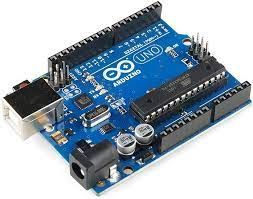
\includegraphics[scale=0.7]{./Figuras/arduino_uno.jpeg}
\caption{Arduino Uno R3}
\label{fig:arduinouno}
\vspace*{-10pt}
\end{figure}

%	Sección tres: Placas Raspberry Pi
\section{Placas Raspberry Pi}
\lhead[\thepage]{\thesection. Placas Raspberry Pi}
Raspberry Pi es una marca (figura \ref{fig:raspi_logo}) de micro computadores de hardware libre, que comenzó como proyecto para llevar a la educación  de escolares ingleses conceptos de la computación, de la programación y de la electrónica, y que luego la comunidad Maker y algunas compañías adoptaron, pues vieron el potencial para crear dispositivos, sensores, actuadores, robots entre otros y para poder llevar a cabo prototipos funcionales de dispositivos y de productos muy rápidamente. Su bajo costo de \$35 por la placa mas costosa y facilidad de uso, han facilitado la adopción de este micro computador por personas en todo el mundo.

\begin{figure}[htb]
\centering

\includegraphics[scale=0.65]{./Figuras/raspi_logo.png}
\caption{Logo de la marca Raspberry Pi}
\label{fig:raspi_logo}
\vspace*{-10pt}
\end{figure}

Este es un proyecto llevado a cabo con la Raspberry Pi Foundation\cite{RaspberryPi} desde el año 2012 ofreciendo hasta el día de hoy siete modelos distintos de placas, con procesadores ARM, memoria RAM que va desde los 256MB hasta 1GB y cuya memoria es de carácter externo usando tarjetas MicroSD en la mayoría de los modelos y cuyo consumo no es mayor al de 2,5 amperios. Los modelos son:
\begin{itemize}
\item Raspberry Pi Modelo A: Fue el primer modelo de Raspberry Pi en salir al mercado, en el año 2012. Basado en un SoC Broadcom BCM28235, cuyo procesador es un ARM11 32 bits a 700MHz, Gráficas Broadcom VideoCore IV, con 256MB de memoria RAM, un puerto USB, una salida HDMI, un conector RCA, una entrada CSI para un modulo de cámara, y sin características de conectividad alguna por defecto. Para el almacenamiento se usan tarjetas SD. 
\item Raspberry Pi Modelo B/B+: También del año 2012, es una variante del Modelo A, trajo consigo diversas mejoras, como la inclusión del doble de memoria RAM, pasando de 256MB a 512MB. Trajo consigo un puerto USB más y un conector Ethernet (RJ-45) Se mantuvo tanto su tamaño como su coste. No hubo variaciones en el procesador ni en la gráfica. Tiempo después se lanzo el Modelo B+, que incluyó 4 puertos USB y pasó de usar una SD a una MicroSD.
\item Raspberry Pi 2 Modelo B: Lanzada en 2014 es el primer modelo que no incluye el mismo procesador usado en los tres anteriores: se sustituye por uno de la misma marca, pero de modelo BCM2836 con lo cual pasa de ser de un núcleo a cuatro, y de 700MHz a 900MHz, no obstante emplea la misma gráfica, la VideoCore IV. Dobla la cantidad de memoria RAM, pasando de 512MB a 1GB de memoria (también compartida con la gráfica). También incluye 40 pines GPIO, y mantiene los cuatro puertos USB. Suprime la conexión RCA.
\item Raspberry Pi 3 Modelo B: Sale al mercado en el año 2016, renovando procesador, una vez más de la compañía Broadcom, siendo un procesador de cuatro núcleos al igual que el modelo anterior, pero pasa de 900MHz a 1.20GHz,  manteniendo la RAM en 1GB. Su mayor novedad fue la inclusión de WiFi y Bluetooth (4.1 Low Energy) sin necesidad de adaptadores.
\item Raspberry Pi Zero: Fue el primer modelo miniaturizado de las Raspberry Pi, teniendo un tamaño un poco mayor a un Pen Drive. Lanzado en 2015 con un coste de 5 dólares, es una 40\% más potente que el primer modelo de Raspberry. Tiene un CPU Broadcom BCM2835, que funciona a 1GHz con dos núcleos. Posee 512MB de RAM, y comparte la gráfica VideoCore IV. Debido a su tamaño sustituye el puerto HDMI por MiniHDMI, manteniendo así las prestaciones. Tampoco usa USB estándar, sino que tiene dos MicroUSB, uno de alimentación y otro de datos. Posee salida RCA, pero en vez de por clavija son solo dos conectores integrados en la placa. Usa MicroSD como sistema de almacenamiento.(figura \ref{fig:rpizero})

\begin{figure}[htb]
\centering
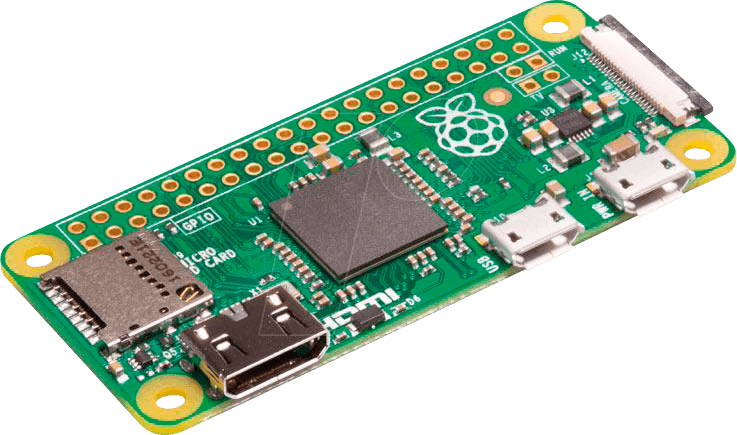
\includegraphics[scale=0.25]{./Figuras/rpizero.png}
\caption{Raspberry Pi 4 modelo B}
\label{fig:rpizero}
\vspace*{-10pt}
\end{figure}

\item Raspberry Pi Zero W: Es la sucesora de la Raspberry Pi Zero. la W es por Wireless, ya que la única novedad de esta placa con respecto a su antecesora es la inclusión de WiFi y Bluetooth, por lo que su precio ascendió a 11 dólares.
\item Raspberry Pi 3 Modelo B+: Del mismo modo que para el Raspberry Pi Modelo B, esta es una actualización en términos de rendimiento sobre la Raspeberry Pi 3 Modelo B. Pasa a ser un poco más rápida que su antecesora y ofrece la capacidad de conectarse a Wifi doble banda. Incorpora Bluetooth 4.2 y la velocidad de su puerto ethernet pasa de 100 Mbits/seg a 300 Mbits/seg.
\item Raspberry Pi 3 Modelo A:  Los modelos A+ presentan menores prestaciones a un menor precio. Cuenta con 512 MB de RAM (compartidos con la GPU VideoCore IV), un solo puerto USB y sin puerto de conexión de red ethernet.
\item Raspberry Pi 4 modelo B: Esta versión viene a sustituir a la versiones 3 y cambia los puertos HDMI de tamaño completo por dos puertos microHDMI. Cuenta con la capacidad de manejar una pantalla a 4K a 60 Hz, o dos pantallas 4K a 30 Hz. Se ha incluido por primera vez USB 3.0, y el puerto Ethernet ya no está limitado a 300 Mbps. Tiene un procesador Broadcom nuevo. Es la primera serie que posee 3 variantes disponibles en los que cambia la cantidad de memoria RAM de 2GB, 4GB, y de 8GB (figura \ref{fig:rpi4}).

\begin{figure}[htb]
\centering
\includegraphics[scale=0.05]{./Figuras/rpi4.jpg}
\caption{Raspberry Pi 4 modelo B}
\label{fig:rpi4}
\vspace*{-10pt}
\end{figure}

\item Raspberry Pi 400: Cuenta con una placa personalizada que se deriva de la Raspberry Pi 4 existente, específicamente remodelada para incluirla en un teclado derivado del Raspberry Pi Keyboard. Posee una solución de enfriamiento mas robusta que su contraparte 4 modelo B al poseer una placa de metal ancha para disipar el calor y un conmutador actualizad para la fuente de alimentación que es un poco mas alta que la del Raspberry Pi 4. La computadora cuenta con 4GB de memoria RAM LPDDR4.
\item Raspberry Pi Pico: Anunciada en el 2021, es una placa pequeña y versátil construida con RP2040, un nuevo chip microcontrolador diseñado por Raspberry Pi Fundation. Este modelo está gobernada por un pequeño SoC que cuenta con un procesador dual core ARM Cortex M0+ funcionando a 133 MHz, acompañado de 264 KB de RAM y 2 MB de almacenamiento integrado.
\item Raspberry Pi 5: La mas nueva de las versiones del Raspberry Pi existentes al momento de la escritura de esta investigación representa el salto de rendimiento sobre el modelo anterior de Raspberry Pi 4. Con un procesador  Broadcom BCM2712 casí duplica la frecuencia del CPU con respecto a su predecesora, ademas de contar ahora con una nueva GPU VideoCore VII mucho más rápida con una frecuencia de 800 MHz. Entre otras mejoras.
\end{itemize}
Existen gran variedad de sistemas operativos que pueden ser usados con este micro computador, la mayoría de ellos, basados en Linux, pero también con la posibilidad de instalar Windows 10 (Iot Core) o Android (Android Things).\\

Una característica principal de estas placas es la existencia de 40 pines GPIO, los cuales proveen entradas y salidas digitales para el micro computador con lo que se le puede expandir su s funcionalidades con el uso de sensores (HATs o a través de circuitos eléctricos tradicionales), cuya logica puede ser creada en lenguajes de programación como Python, C++, Java, entre otros.\\

El proyecto ha ganado una comunidad muy amplia al rededor del mundo, que han probado la versatilidad que posee este micro computador en proyectos de toda índole, dando a las personas la capacidad de crear soluciones basadas en el Internet de las Cosas de una forma divertida y a su vez, con calidad y robustez.


%	capitulo cinco
%-----------------------------------------------------------------------------
%	 Marco Aplicativo
%-----------------------------------------------------------------------------

\lhead[\thepage]{Metodología General de Trabajo \thechapter. \rightmark}
\rhead[Metodología General de Trabajo \leftmark]{\thepage}
\part{Marco Aplicativo}
%	Capitulo 6: Metodología General de Trabajo
\chapter{Metodología General de Trabajo}
\markboth{Metodología General de Trabajo}{Metodología General de Trabajo}

\section{Scrum}
\lhead[\thepage]{\thesection. Scrum}
Scrum es una metodología ágil y flexible para gestionar el desarrollo de software. Se basa en construir primero la funcionalidad de mayor valor para el cliente y en los principios de inspección continua, adaptación, auto-gestión e innovación.\cite{scrumsofteng} En Scrum se aplican de manera regular un conjunto de buenas prácticas para trabajar colaborativamente y obtener el mejor resultado posible de un proyecto.\\

Es parte de la filosofía de Scrum el poder realizar entregas parciales y regulares del producto final, priorizadas por el beneficio que aportan al receptor del proyecto. Por ello, Scrum está especialmente indicado para proyectos en entornos complejos, donde se necesita obtener resultados rápidamente, con requisitos son cambiantes o poco definidos, donde la innovación, la competitividad, la flexibilidad y la productividad son fundamentales.\\

En Scrum un proyecto se ejecuta en bloques temporales cortos y fijos (iteraciones que normalmente son de 2 semanas, aunque en algunos equipos son de 3 y hasta 4 semanas, límite máximo de feedback y reflexión). Cada iteración tiene que proporcionar un resultado completo, un incremento de producto final que sea susceptible de ser entregado con el mínimo esfuerzo al cliente cuando lo solicite. El proceso parte de la lista de objetivos/requisitos priorizada del producto, que actúa como plan del proyecto. En esta lista el cliente prioriza los objetivos balanceando el valor que le aportan respecto a su coste y quedan repartidos en iteraciones y entregas.\\  

La actividades que se llevan a cabo bajo la metodología de Scrum son las siguientes:

\begin{enumerate}
\item Planificación de la iteración: En el primer día de cada iteración, el equipo realza una reunión de planificación de la iteración. Esta etapa consiste en una primera fase de selección de requisitos, en la cual el cliente presenta al equipo la lista de requisitos priorizada del proyecto y se responden a las dudas que surgen sobre el dominio de las tareas a realizar y una segunda fase de planificación de la iteración, donde el equipo elabora la listas de tareas necesarias para desarrollar lo que se es requerido para la iteración, ademas de la estimación de esfuerzos por parte de los miembros del equipo.
\item Ejecución de la iteración: Cada día se realiza una reunión con todo el equipo de 15 minutos como máximo para inspeccionar el avance en la realización de las tareas, dependencias u actividades bloqueantes ye insumos pendientes para su culminación. Durante la iteración el Scrum Master (facilitador) se encarga de que el equipo pueda articularse y cumplir los compromisos adquiridos por el equipo.
\item Inspección y adaptación: El ultimo día de la iteración se realiza la reunión de revisión de la iteración. Esta se conforma de dos partes, la demostración en donde el equipo presenta al cliente el/los entregable(s) con los requisitos mínimos acordados y la retrospectiva en la que el equipo analiza si su manera de trabajar ha sido la adecuada, los problemas que han surgido, su solución, de forma que se pueda mejorar de manera continua la productividad.
\end{enumerate}

\section{Control de Versiones de Software}
\lhead[\thepage]{\thesection. Control de Versiones de Software}
Un software de control de versiones es un aquel que permite registrar y gestionar cambios a nivel del código fuente de manera histórica permitiendo retornar a versiones anteriores o comprar diferencias entre ellas.

Esto permite tener:
\begin{itemize}
\item Flujos de trabajo organizados:
\item Descripción de versiones:
\item Colaboración:
\item Historial de cambios: 
\end{itemize}

\subsection{Git}
Git es un sistema de control de versiones moderno, distribuido y seguro que fue desarrollado originalmente por Linus Torvalds en el año 2005. 

Entre sus características principales se destacan:
\begin{itemize}
\item Arquitectura distribuida:
\item Flexibilidad:
\item Seguridad:
\item Rendimiento:
\end{itemize}

\subsubsection{Git-Flow}
Git Flow es una metodología para usar Git en la que se combina ramas de función y ramas principales. Fue popularizado por Vincent Driessen en 2010. Los aspectos clave del modelo Git Flow son:
\begin{itemize}
\item Ramas principales y de desarrollo: En lugar de tener una única rama principal, Git Flow utiliza dos ramas principales:
\begin{enumerate}
\item Main (o Master): Almacena el historial oficial de publicación.
\item Develop: Sirve como rama de integración para las funciones.
\end{enumerate}
\item Ramas de función: Los desarrolladores crean ramas de función para trabajar en características específicas. Estas ramas se fusionan con develop cuando la función está completa.
\item Ramas de publicación y corrección de errores:
\begin{enumerate}
\item Release Branches: Se crean a partir de develop para preparar una nueva versión. Aquí se realizan pruebas finales y se corrigen errores antes de la publicación.
\item Hotfix Branches: Se utilizan para corregir errores críticos en la versión actual de producción. Se crean a partir de main y se fusionan tanto con main como con develop.
\item Versionado y etiquetado: Git Flow simplifica la gestión de versiones al asignar números de versión a las confirmaciones en main y etiquetarlas.
\end{enumerate}
\end{itemize}

\section{Herramientas de Desarrollo}
\lhead[\thepage]{\thesection. Herramientas de Desarrollo}
A continuación se detalla aquellas herramientas de hardware y de software utiizados durante el desarrollo de este trabajo de investigación.

\subsection{Herramientas de Hardware}
Dado el enfoque de tener un grupo de dispositivos IoT que pudiesen obtener data real del entorno en donde fuesen desplegados, se obtuvo un conjunto de placas programables, microcomputadores y microcontroladores, así como también de sensores y actuadores para poder crear prototipos funcionales. Se contó con cuatro placas programables de distinta índole:
\begin{itemize}
\item Dos Raspberry Pi modelos 3 B.
\item Un Raspberry Pi Zero.
\item Un Arduino Uno R3.
\end{itemize}

Entre los sensores y actuadores a integrar a esos dispositivos se ha contado con los siguientes elementos:
\begin{itemize}
\item Dos sensores de movimiento PIR HC-SR501.
\item Un sensor de test de nivel de agua Robodo Sen18.
\item Un sensor de temperatura DS1820.
\item Dos leds RGB.
\item Una fotorresistencia (LDR).
\item Un sensor de temperatura y humedad DHT11.
\item Dos leds color verde.
\item Dos leds color rojo.
\item Seis leds color blanco.
\item Un sensor de intensidad lumínica TSL2561.
\item Un buzzer HW-508.
\item Una pantalla LCD 16x2 I2C Hd44780.
\item Un Lector de tarjetas RFID RC522.
\item Un llavero RFID 100.
\item Una tarjeta RFID programable. 
\item Una cámara RaspiCam V1.  
\end{itemize}

Por otro lado para el desarrollo de software se hizo uso de un computador con las siguientes características:
\begin{itemize}
\item CPU
\item RAM
\item Almacenamiento
\item Sistema Operativo
\end{itemize}

Finalmente el software desarrollado fue desplegado en uno de los dispositivos Raspberry Pi 3 modelo B cuyas características son:
\begin{itemize}
\item CPU
\item RAM
\item Almacenamiento
\item Sistema Operativo
\end{itemize}

\subsection{Python}
Python es un lenguaje de programación de alto nivel, multiplaforma,  débilmente tipado de propósito general, multiparadigma e interpretado\cite{whatspython}, creado por Guido Van Rossum. Su filosofía se basa en el poder crear código que sea muy legible, con una sintaxis simple, utilizando indentaciones para delimitar bloques de código, mas corto y potente que en otros lenguajes de programación.\cite{Guido}\\

Se dice que Python es un lenguaje que viene con "pilas puestas"\cite{pep206}, es decir, que de por si, posee un conjunto de funciones amplio para afrontar cualquier tipo de situación dentro de las librería estándar del lenguaje y destaca en su facilidad para aprender y alta portabilidad y es usado en un una gran cantidad de aplicaciones, que van desde el área web, pasando por la ciencia de datos, la inteligencia artificial y la programación de dispositivos.  

\begin{figure}[ht]
\centering

\includegraphics[width=0.4\textwidth]{Figuras/python-logo.png}
\caption{\label{fig:python-logo}Logo de Python}
\vspace*{-10pt}
\end{figure}

\subsection{Django}
Django es un framework web de alto nivel que permite el desarrollo rápido de sitios web seguros y mantenibles. Desarrollado por programadores experimentados, Django se encarga de gran parte de las complicaciones del desarrollo web, por lo que puedes concentrarte en escribir tu aplicación sin necesidad de reinventar la rueda. Es gratuito y de código abierto

\subsection{Bases de datos}
Para el desarrollo de la aplicación web se desplegaron dos bases de datos para poder aprovechar las caracteristicas de los datos y flujos involucrados:
\begin{itemize}
\item Una base de datos Postgresql para la gestión de los datos y elementos de la aplicación web en si misma.
\item Una base de datos InfluxDB para almacenamiento de la información registrada por la operación de los sensores y actuadores de los dispositvos IoT.
\end{itemize}

\subsubsection{Postgresql}
Es un sistema de gestión de bases de datos relacional orientado a objetos y de código abierto. Sus principales caracteristicas son:
\begin{itemize}
\item Alta concurrencia.
\item Amplia cantidad de tipos nativos.
\end{itemize}

\subsubsection{InfluxDB}
Es una base de datos de series temporales de código abierto desarrollada por InfluxData, utilizada para almacenar y recuperar datos de series temporales en áreas como monitoreo de operaciones, métricas de aplicaciones, datos de sensores de Internet de las Cosas y análisis en tiempo real. Está escrita en el lenguaje de programación Rust.

\subsection{Eclipse Mosquitto}
Eclipse Mosquitto es un broker de mensajes de código abierto que implementa las versiones 5.0, 3.1.1 y 3.1 del protocolo MQTT. Es ligero y adecuado para todos los dispositivos, desde computadoras de placa única de baja potencia hasta servidores completos. Esta escrito en el lenguaje de programación C.

\subsection{Grafana}
Grafana es una plataforma de visualización de código abierto que permite generar métricas, registros y trazas de datos de otras aplicaciones a través del uso de graficos y tablas organizados en dashboards. Permite consultar, visualizar, configurar alertas y comprender tus métricas, sin importar dónde se almacenen. 

\subsection{Node-Red}
Node-RED es una herramienta de programación que te permite conectar, integrar y automatizar dispositivos de hardware, APIs y servicios en línea. Su editor basado en paneles dentro del navegador facilita la creación de flujos mediante una amplia variedad de nodos, que luego se pueden implementar en su entorno de ejecución al mismo tiempo de manera sencilla.

\subsection{Docker}
Docker es una plataforma de código abierto que simplifica y automatiza el proceso de construir, desplegar y gestionar contenedores. Los contenedores son componentes estandarizados y ejecutables que combinan el código de la aplicación con las dependencias del sistema operativo.

\section{Adaptación del Marco Metodológico}
Para llevar a cabo la investigación propuesta, se decidió adaptar la metodología de forma que está favoreciera el desarrollo de los diversos elementos que se requerían. De esta manera se acordó hacer uso de lo siguiente:
\begin{itemize}
\item Sprints de dos semanas de duración.
\item Reuniones mensuales para realizar retrospectiva, sprint review y planificación de actividades para los siguientes sprints. Reunión en formato daily cada semana para comentar avances, bloqueos y recursos requeridos.  
\item Hacer entregas incrementales basadas en la adición de features y correcciones de código cada final de sprint.
\item Kick off del proyecto para el mes de septiembre del 2018.
\item Duración estimada del desarrollo de los dispositivos y de la aplicación web de 9 sprints (18 semanas).
\item El profesor Antonio Russoniello en calidad de tutor del trabajo especial de grado, asume el rol de Scrum Master. 
\item El bachiller Pedro Boll asume el desarrollo. 
\end{itemize}
Con ello definido, se presentan las siguientes actividades para el desarrollo y culminación del proyecto según los objetivos generales y especificos en la  tabla \ref{tabla:actividades_desarrollo}, junto con su duración aproximada.

\begin{table}[!htb]
\centering
\begin{tabular}{| m{4.5cm}| m{5cm}| m{4.5cm}|}
\hline
\multicolumn{3}{|c|}{Actividades de desarrollo} \\
\hline 
\centering Actividad & \centering Descripción & \centering Tiempo Estimado \tabularnewline \hline

Diseño y prototipado de dispositivos & 2 & dos semanas/un sprint \\ \hline

Desarrollo de scripts de sensores, actuadores y comunicación de datos & 2 & dos semanas/un sprint \\ \hline

Captura de datos de dispositivos & 2 & doce semanas/seis sprint \\ \hline

Instalación y despliegue de Infraestructura & 2 & una semana/medio sprint \\ \hline

Desarrollo de entorno back-end para proceso de obtención de datos & 2 & una semana/medio sprint  \\ \hline

Documentación de proceso de obtención de datos & 2 & una semana/medio sprint \\ \hline

Diseño de aplicación web & 2 & una semana/medio sprint \\ \hline

Implementación base de aplicación web (módulo inicial, templates base) & 2 & una semana/medio sprint \\ \hline

Desarrollo de módulo de gestión de aplicación & 2 & una semana/medio sprint \\ \hline

Desarrollo de módulo de visualización de datos & 2 & una semana/medio sprint \\ \hline

Desarrollo de módulo de control y automatización de flujos de dispositivos & 2 & una semana/medio sprint \\ \hline

Desarrollo de módulo de comunicación y redes & 2 & una semana/medio sprint \\ \hline

Documentación de aplicación web & 2 & una semana/medio sprint \\ \hline

Pruebas end to end del proyecto de investigación & 2 & cuatro semanas/dos sprint \\ \hline

Recolección de resultados & 2 & dos semanas/un sprint \\ \hline

\end{tabular}
\caption{Actividades sugeridas para el desarrollo del trabajo especial de grado}
\label{tabla:actividades_desarrollo}
\end{table}
 
%	Capitulo seis
%-----------------------------------------------------------------------------
%	 Diseño e Implementación
%-----------------------------------------------------------------------------

\lhead[\thepage]{Diseño e Implementación \thechapter. \rightmark}
\rhead[Diseño e Implementación \thechapter.1 \leftmark]{\thepage}

%	Capitulo 6: Diseño e Implementación
\chapter{Diseño e Implementación}
\markboth{Diseño e Implementación}{Diseño e Implementación}
En este capitulo se presenta a partir del problema planteado una solución basada en una aplicación web que es capaz de poder tomar los datos de dispositivos IoT entre sensores y actuadores con los que interactuar, a través de la integración de diversas herramientas de visualización y control, incluyendo la posibilidad tanto de presentar indicadores de datos en tiempo real, así como también interactuar con data histórica para su análisis.\\

Todas las tecnologías aquí presentadas son software y hardware libre por lo que pueden ser adaptadas rápidamente según los requerimientos funcionales del problema y cumplen con legislativa local para poder ser exploradas a fondo. 

%	Sección uno: Diseño de la solución
\section{Diseño de la solución}
\lhead[\thepage]{\thesection. Diseño de la solución}
El diseño propuesto para examinar la solución al problema planteado pasa por dos etapas:
\begin{itemize}
\item Prototipos de uno o más dispositivos IoT que sean capaces de generar información real de su entorno, explorando los métodos más adecuados para poder llevar a cabo la tarea de transmitir información, así como explorar las posibilidades de procesamiento de cada dispositivo.
\item Aplicación web que incluya la posibilidad de visualizar los datos, monitorear y controlar los dispositivos IoT que se encuentren registrados. Para ello se integraran una serie de herramientas de software que aprovechen las mejores características de su diseño para poder cumplir con los objetivos planteados.
\end{itemize}

A continuación se presentan de manera detallada el diseño de ambos elementos:

\subsection{Prototipos de Dispositivos IoT}
Para los prototipos de los dispositivos IoT se contó con cuatro placas programables de distinta índole:
\begin{itemize}
\item Dos Raspberry Pi modelos 3 B.
\item Un Raspberry Pi Zero.
\item Un Arduino Uno R3.
\end{itemize}

Por el lado de los sensores y actuadores a integrar a esos dispositivos se ha contado con los siguientes elementos:
\begin{itemize}
\item Dos sensores de movimiento PIR HC-SR501.
\item Un sensor de test de nivel de agua Robodo Sen18.
\item Un sensor de temperatura DS1820.
\item Dos leds RGB.
\item Una fotorresistencia (LDR).
\item Un sensor de temperatura y humedad DHT11.
\item Dos leds color verde.
\item Dos leds color rojo.
\item Seis leds color blanco.
\item Un sensor de intensidad lumínica TSL2561.
\item Un buzzer HW-508.
\item Una pantalla LCD 16x2 I2C Hd44780.
\item Un Lector de tarjetas RFID RC522.
\item Un llavero RFID 100.
\item Una tarjeta RFID programable. 
\item Una cámara RaspiCam V1.  
\end{itemize}

Dado que los dispositivos Raspberry Pi pueden usar un sistema operativo completo estos pueden operar de manera independiente a otros dispositivos, no siendo el caso del dispositivo Arduino Uno se complementa su integración haciendo uso de una computadora Apple iBook G4 para poder recibir y enviar la data de manera inalámbrica.\\

Siendo la idea examinar variables y comportamientos de dispositivos en un ambiente de un hogar inteligente junto con la variedad de placas programables, sensores y actuadores disponible se sugieren la creación de 4 prototipos de dispositivos IoT distintos:

\begin{itemize}
\item Un prototipo de dispositivo IoT usando Arduino Uno (junto al computador iBook G4) para representar un artefacto que se coloque en exteriores para obtener y representar variables ambientales y de recursos comunes en esas áreas. Para ello se destinan un sensor PIR HC-501, un sensor de test de nivel de agua Robodo Sen18, Un sensor de temperatura DS1820, un Led RGB para representar de manera visual la temperatura y una fotorresistencia LDR de 10K (véase figura: \ref{fig:arduino1}).
\begin{figure}[htb]
\centering
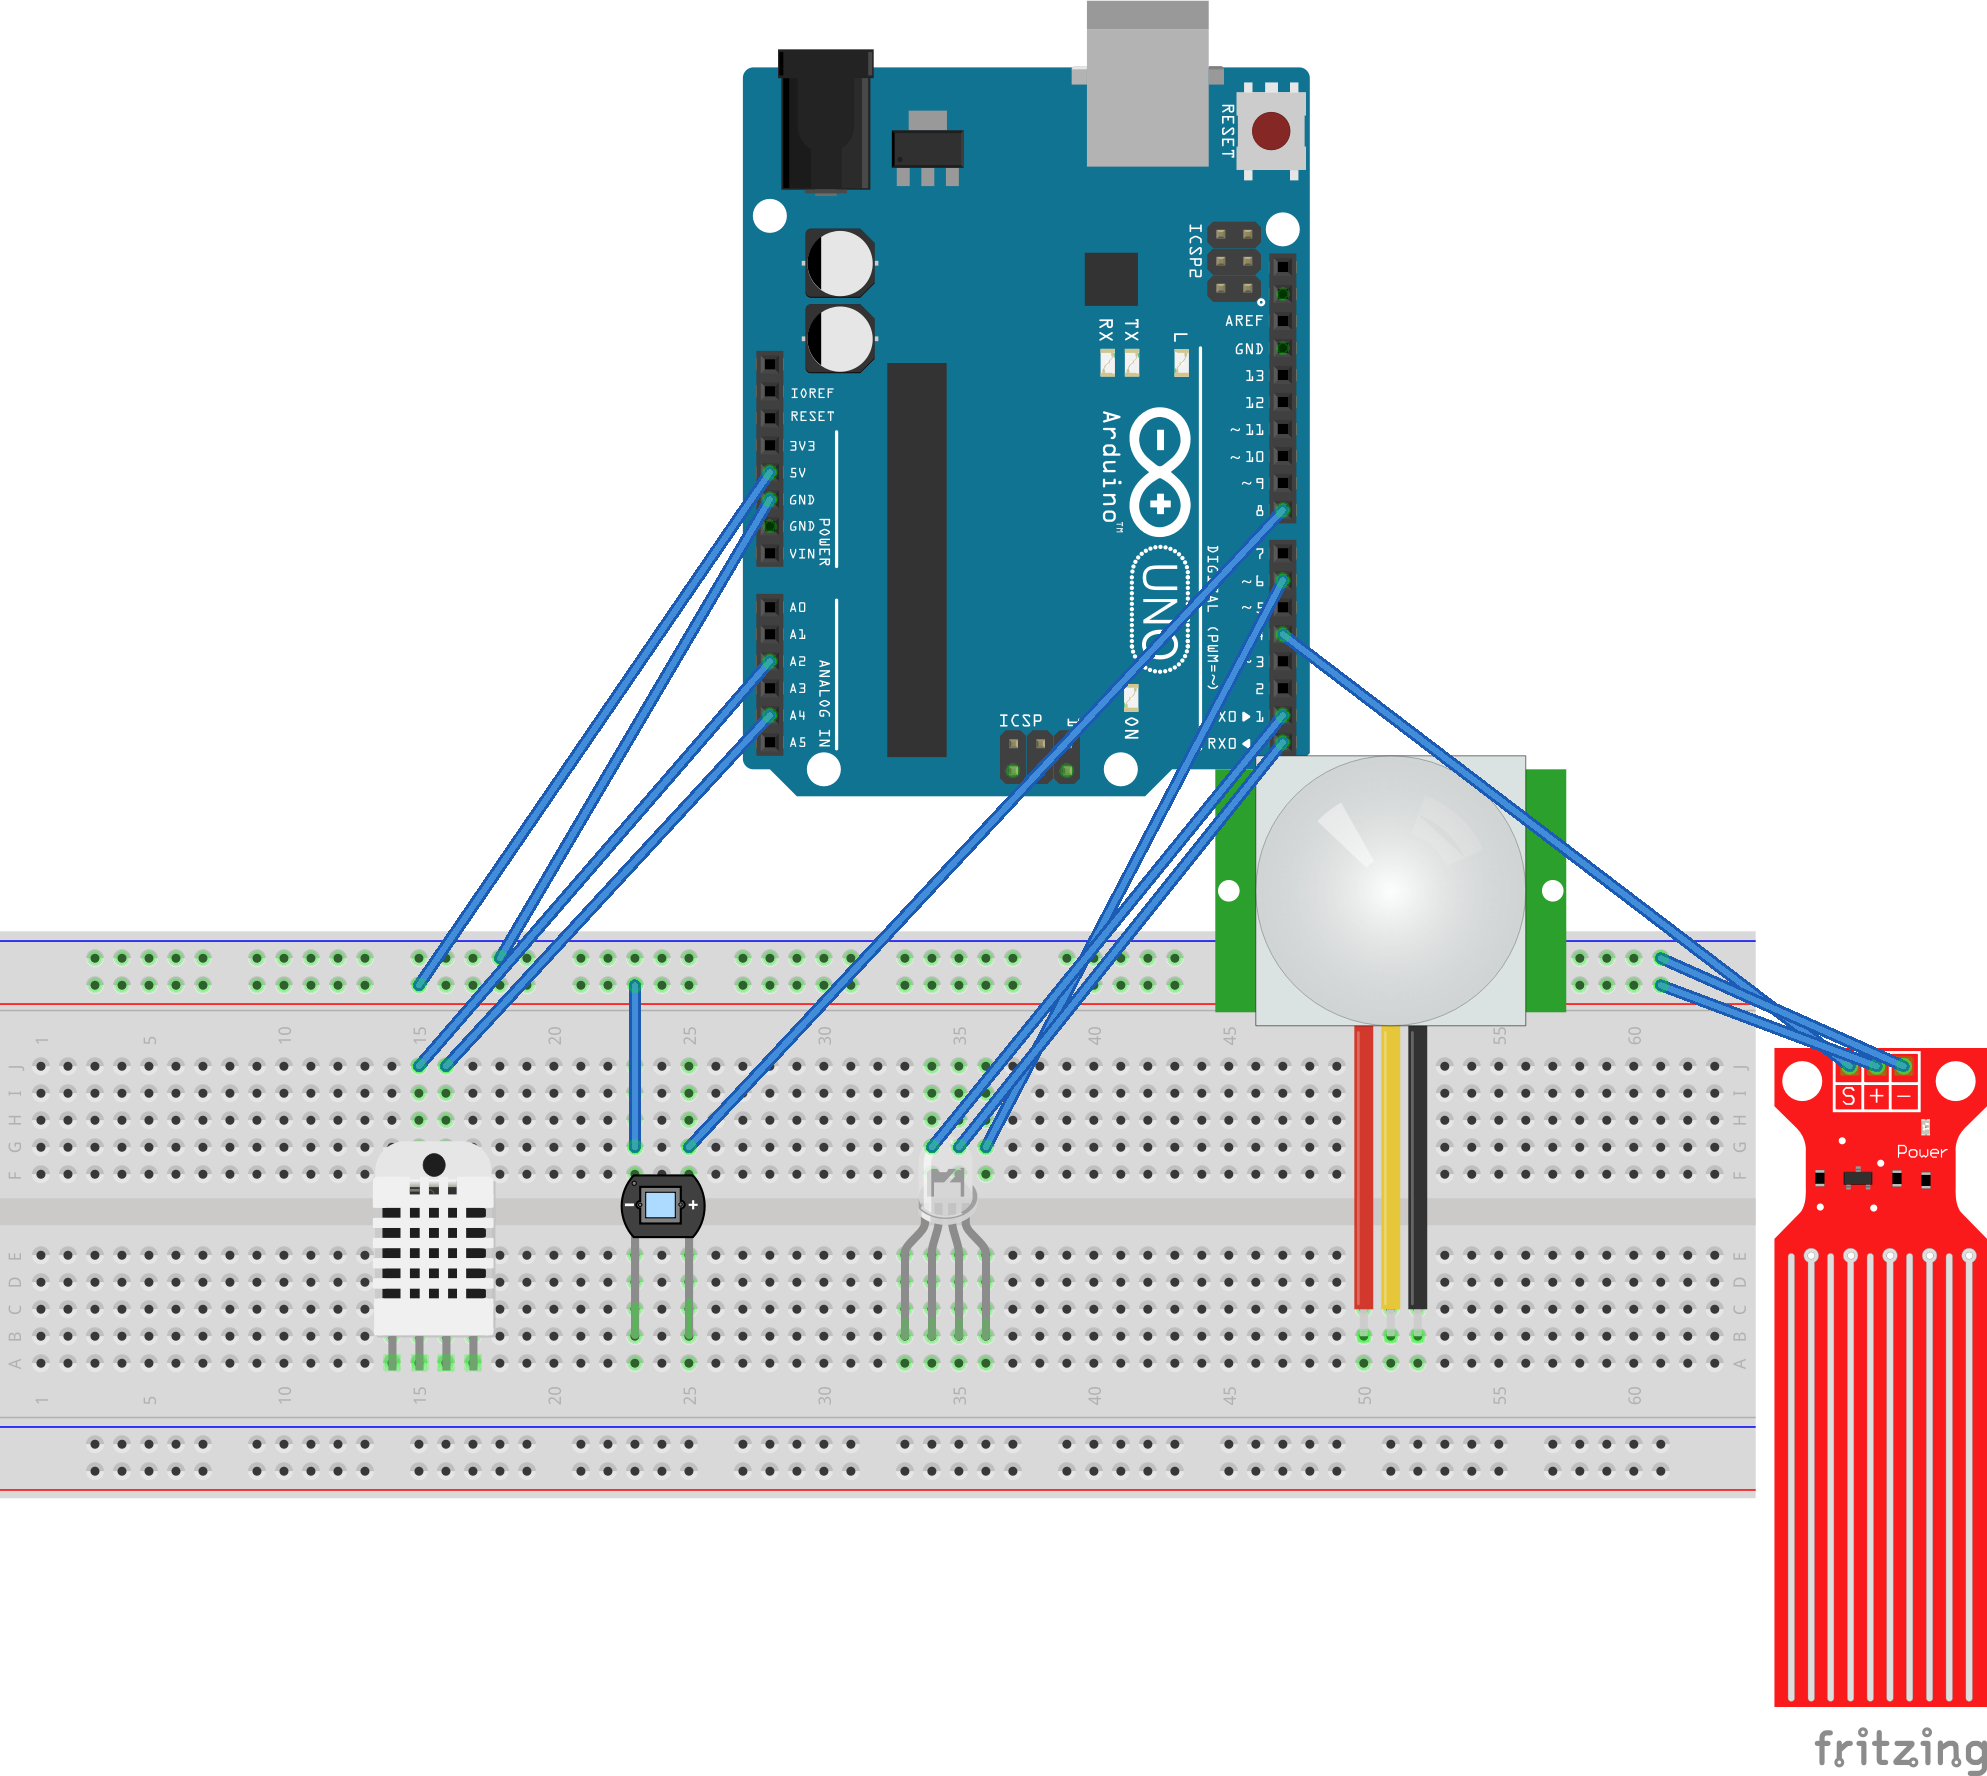
\includegraphics[scale=0.5]{./Figuras/arduino1.png}
\caption{Prototipo de dispositivo exterior usando Arduino Uno}
\label{fig:arduino1}
\vspace*{-10pt}
\end{figure}

\item Un prototipo de Dispositivo IoT usando un Raspberry Pi 3 Modelo B para representar un artefacto que se coloca en un espacio interior para obtener y representar variables ambientales y recursos comunes en el área. Para ello se harán uso de un sensor de temperatura y humedad DHT11, un Led RGB para representar de manera visual la temperatura, un sensor de medición de distancia usando ultrasonido HC-SR504, un led rojo y un led verde operacionales para indicar presencia de movimiento con el sensor de movimiento, un un buzzer y un servomotor que dada una cierta distancia con el sensor de movimiento se accionaran y a su vez tocara una melodía, un conjunto de 3 leds blancos para representar bombillos en una habitación y por último un sensor de intensidad lumínica TSL2561 para medir la intensidad de la luz en la habitación.(véase figura: \ref{fig:rpi3javier}).
\begin{figure}[htb]
\centering
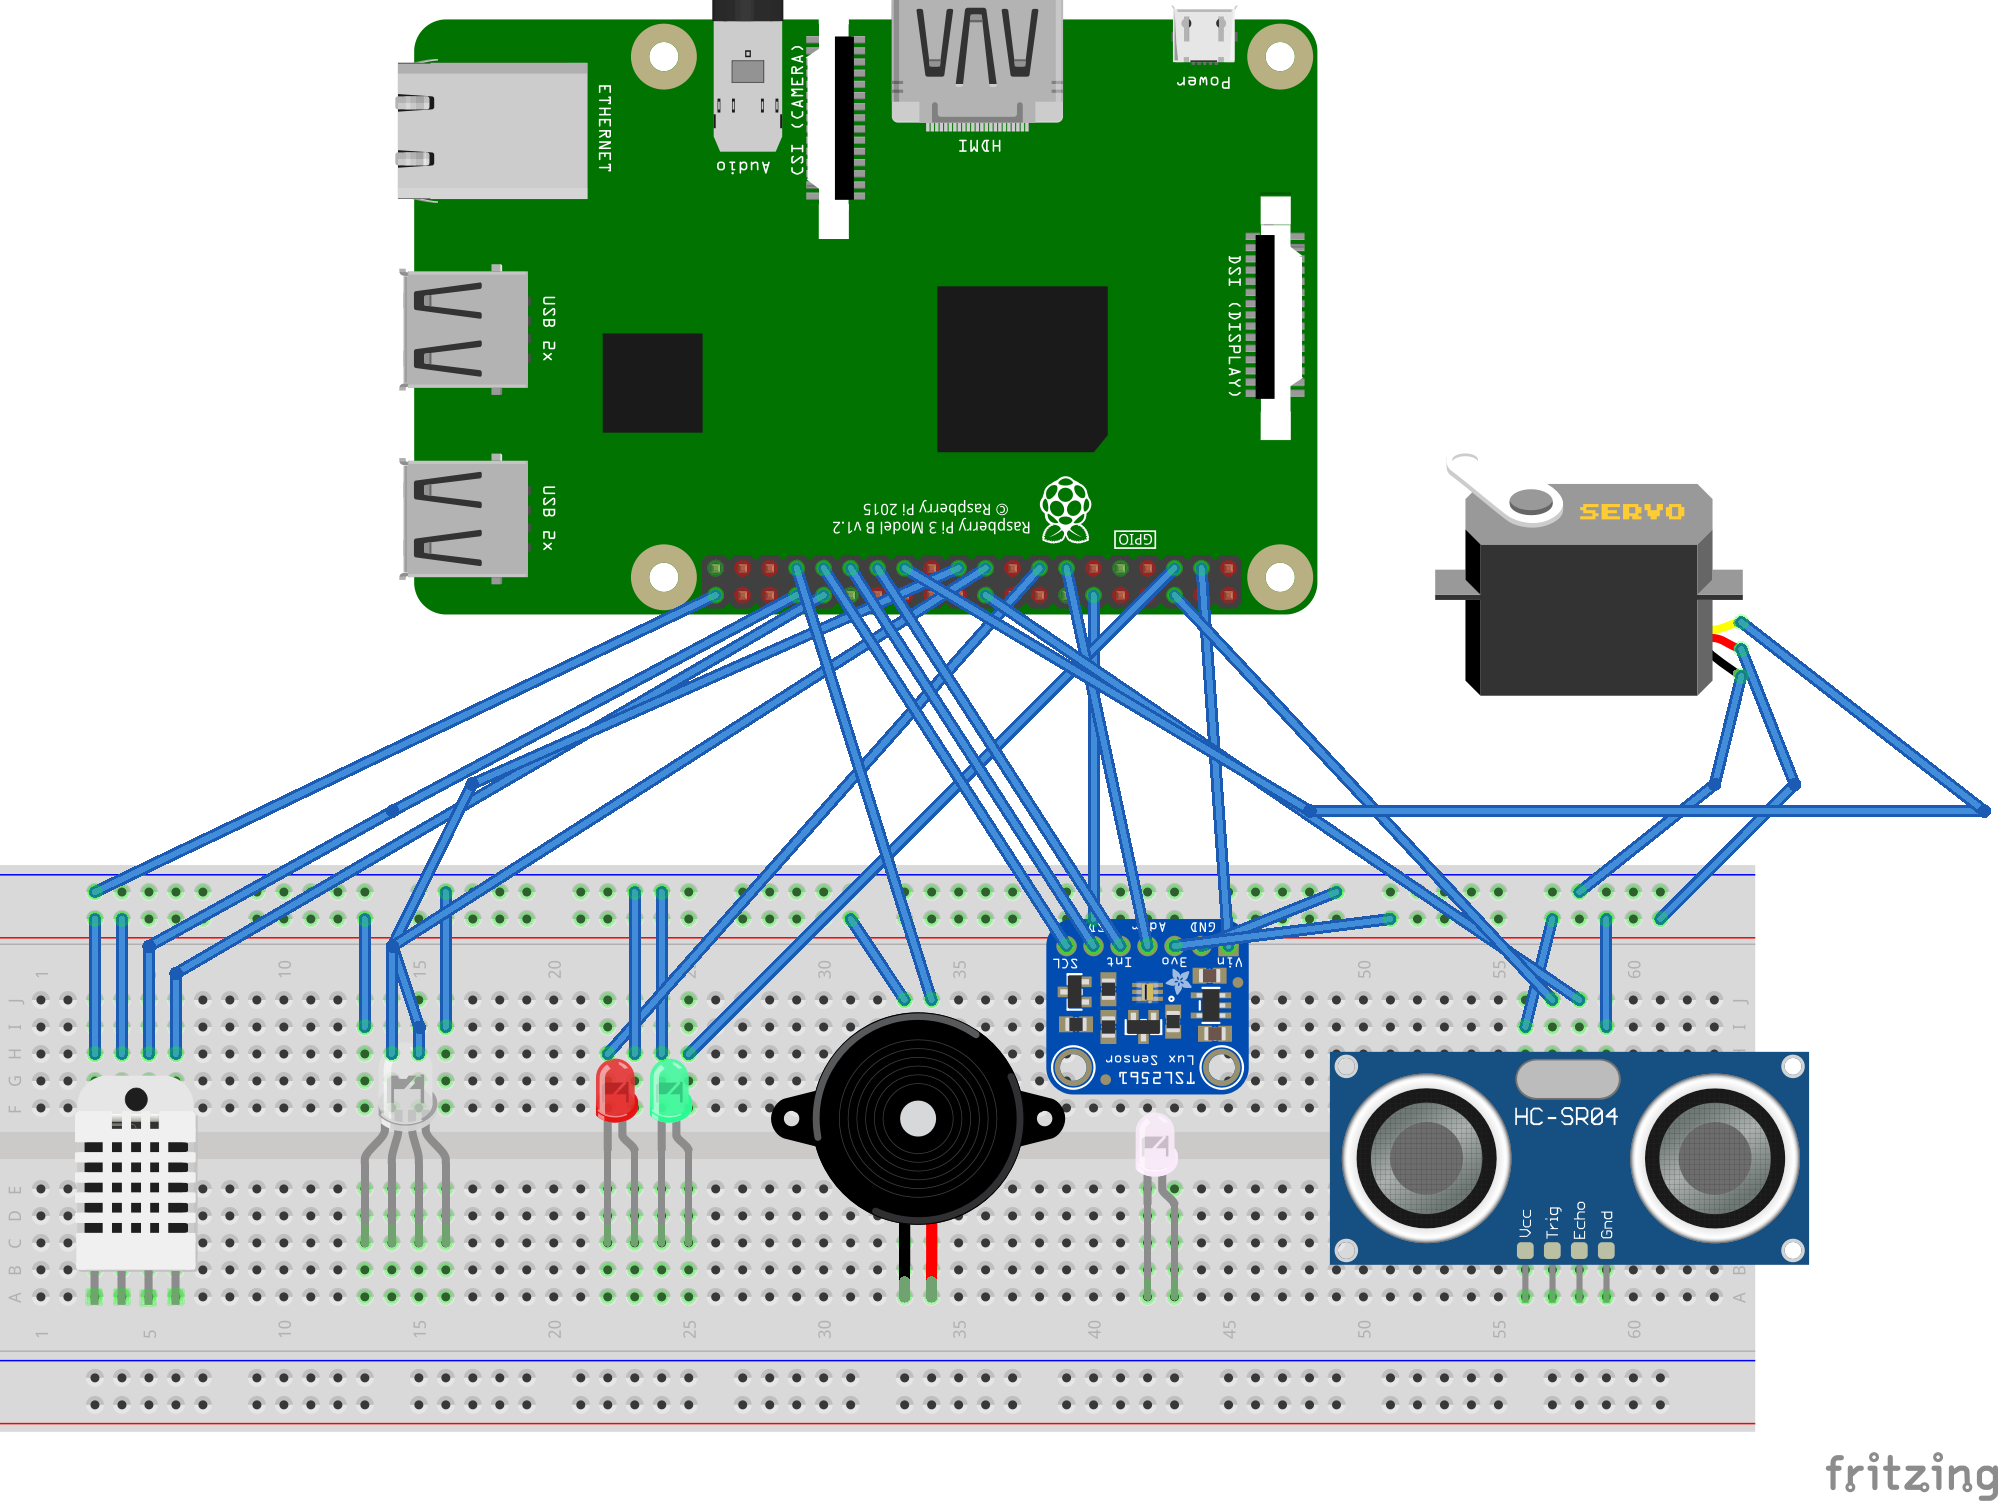
\includegraphics[scale=0.5]{./Figuras/rpi3javier.png}
\caption{Prototipo de dispositivo interior usando un Raspbery Pi 3 modelo B}
\label{fig:rpi3javier}
\vspace*{-10pt}
\end{figure}

\item Un prototipo de Dispositivo IoT usando un Raspberry Pi zero para representar un artefacto pensado para en variables de seguridad y acceso que se coloca en un espacio interior. Para ello se harán uso de un lector RFID RC522, una pantalla LCD para representar la hora y darle la bienvenida al usuario, un led rojo y un led verde operacionales para indicar existencia de movimiento gracias a un sensor PIR HC-SR501, 3 leds blancos para representar bombillos (que se activen con movimiento).(véase figura:\ref{fig:rpizero_diagram}).
\begin{figure}[htb]
\centering
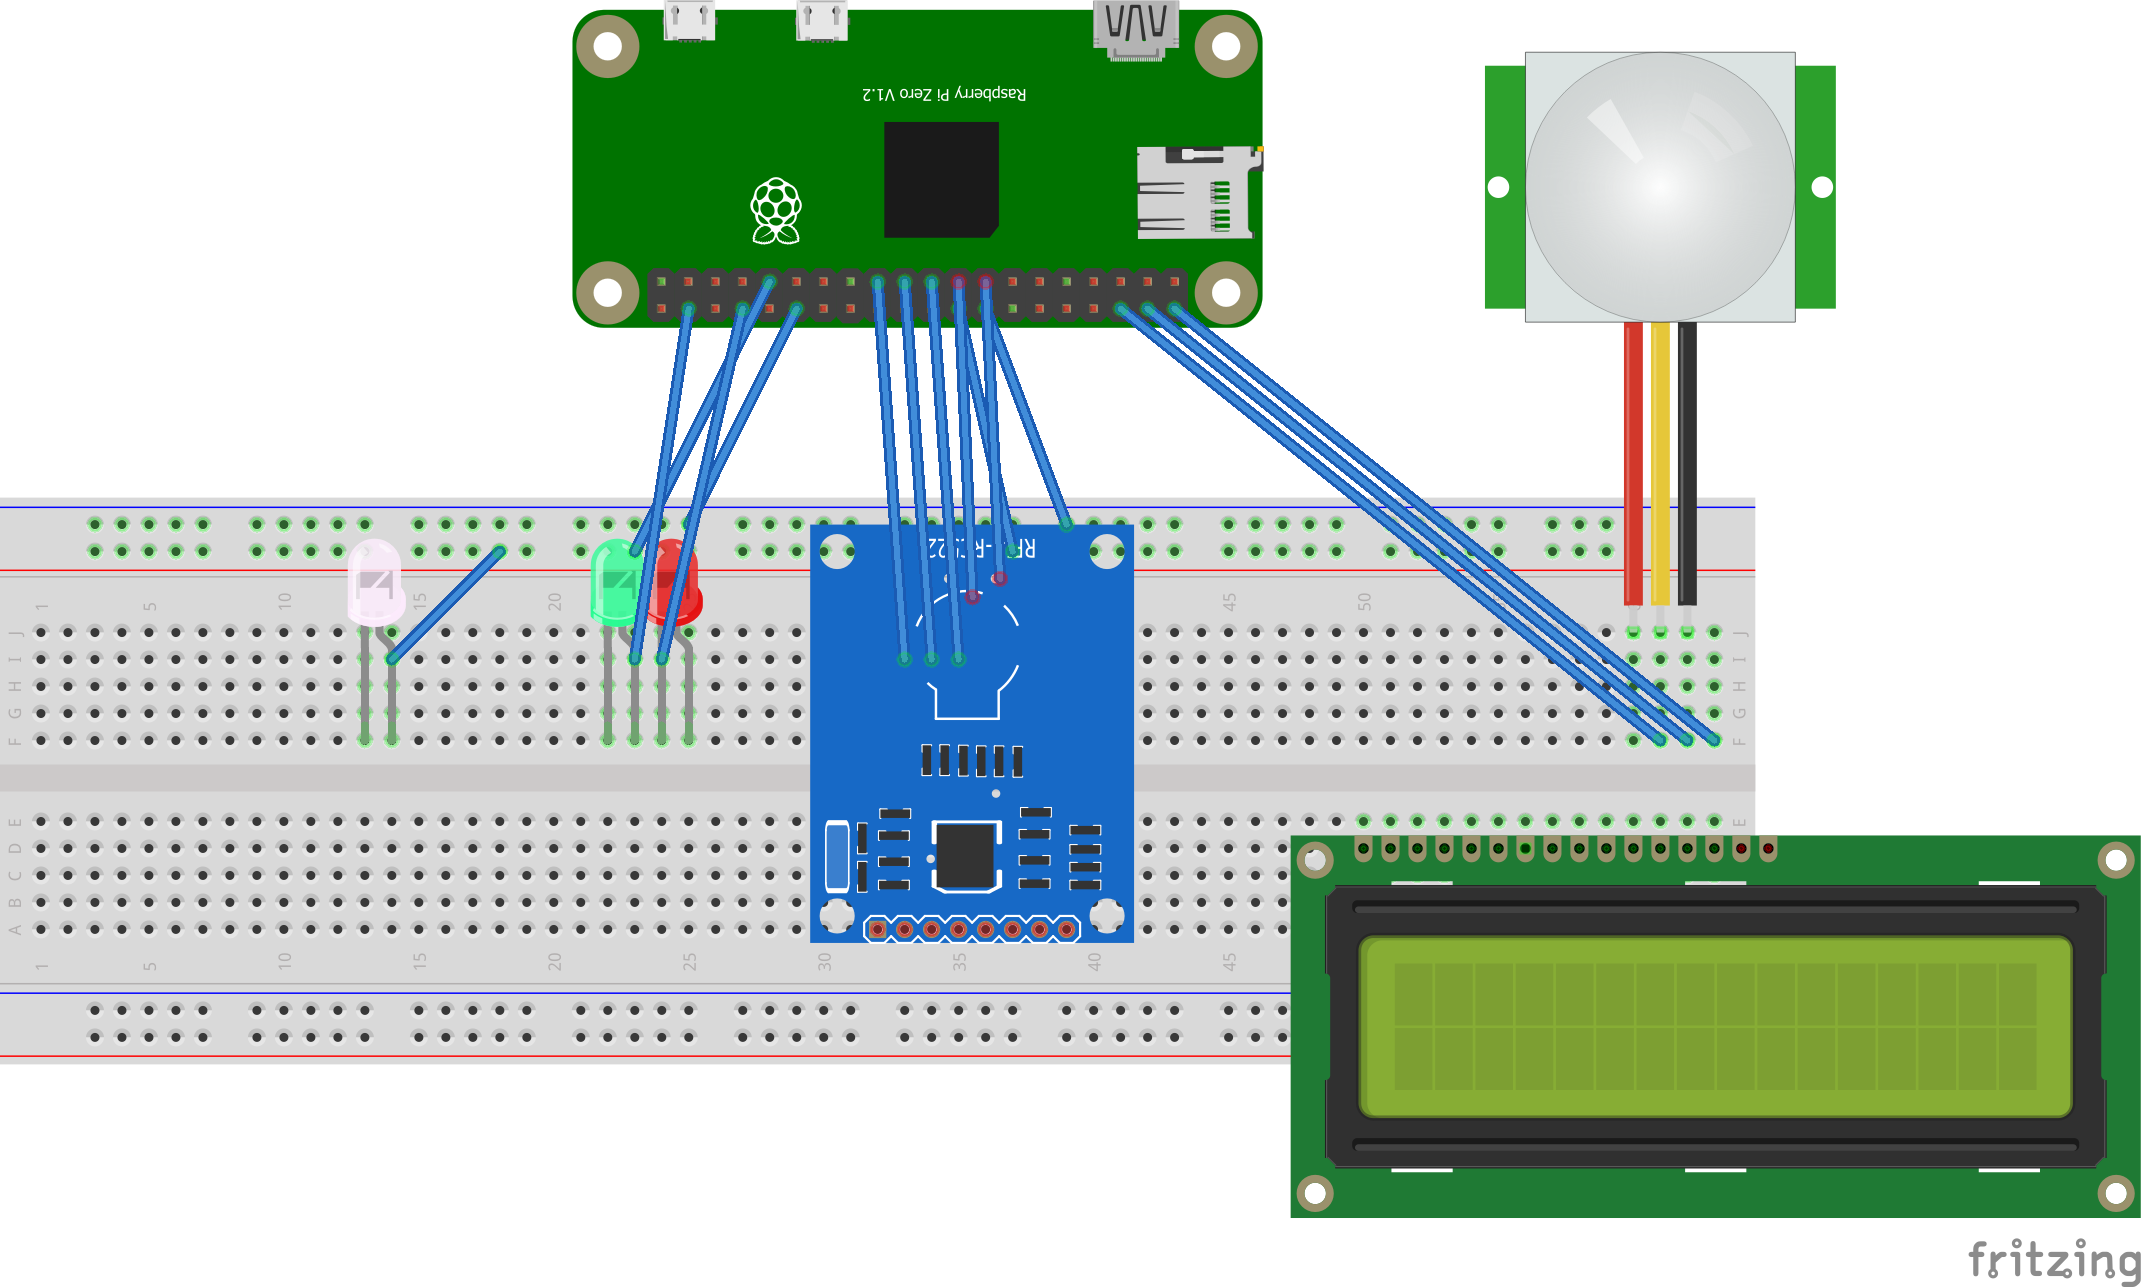
\includegraphics[scale=0.5]{./Figuras/rpizero_diagram.png}
\caption{Prototipo de dispositivo de seguridad usando un Raspbery Zero}
\label{fig:rpizero_diagram}
\vspace*{-10pt}
\end{figure}

\item Un prototipo de dispositivo IoT usando un Rapsberry Pi 3 Modelo B para representar una cámara inteligente capaz de detectar rostros de personas registradas y de desconocidos para alertar una posible intrusión usando un modelo de inteligencia artificial para ello. Se destina la cámara RaspiCam v1 para este particular.(véase figura:\ref{fig:rpipeter}). También dadas las capacidades computacionales de esta placa programable se establece que pueda usarse como punto de acceso para los otros prototipos y lugar de despliegue de la herramienta web HAMACA para visualización, monitoreo y control de los prototipos. 
\begin{figure}[htb]
\centering
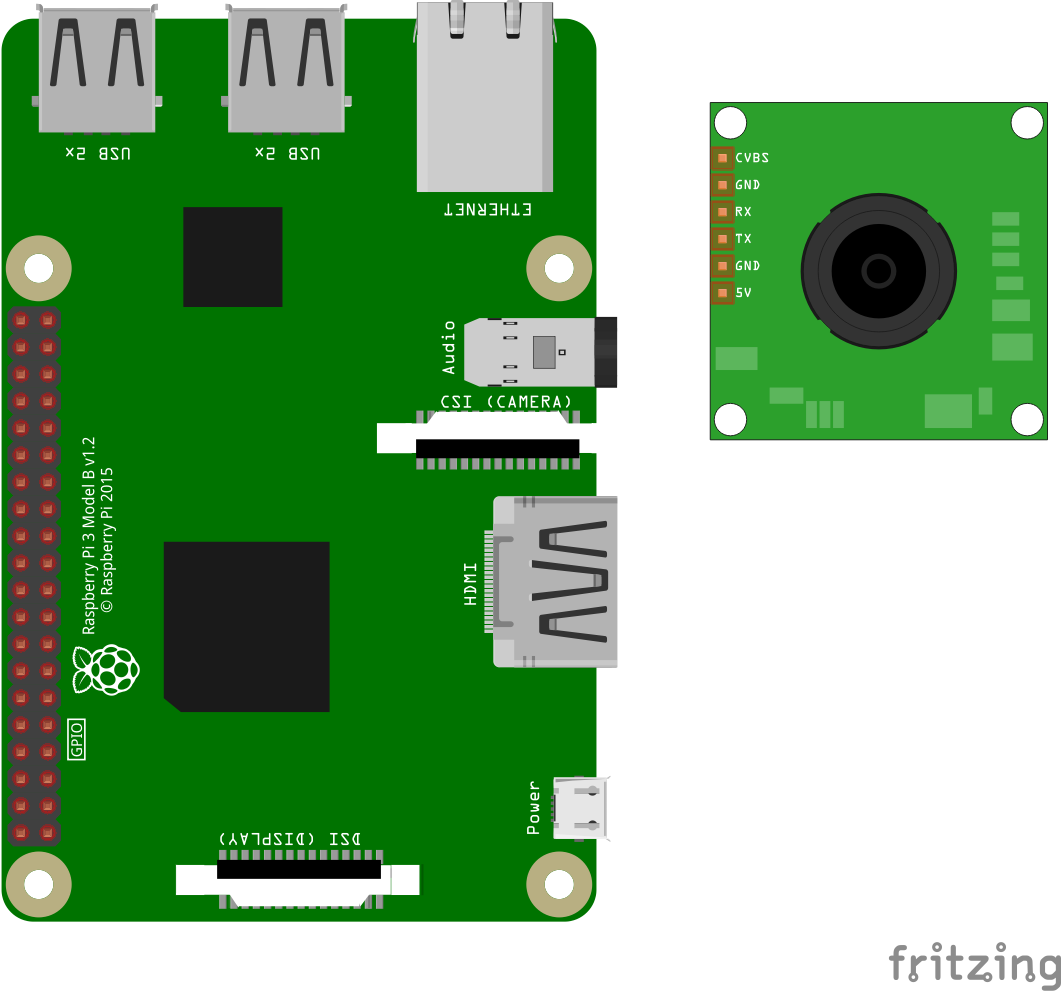
\includegraphics[scale=0.6]{./Figuras/rpipeter.png}
\caption{Prototipo de dispositivo de cámara de inteligente usando un Raspbery Pi 3 modelo B}
\label{fig:rpipeter}
\vspace*{-10pt}
\end{figure}

\end{itemize}

Con esta gama de distintos prototipos planteados para escenarios diferentes se hará obtención de data y generar acciones automáticas dependiendo del contexto que estos datos provean.  

\subsection{Software de Visualización, monitoreo y control HAMACA}
La parte mas importante del planteamiento del problema se traduce en la falta de soluciones que permitan visualizar datos históricos y en tiempo real, junto con la capacidad de monitorear el estado de los dispositivos y la posibilidad final de controlarlos y establecer rutinas mas allá de su programación inicial.\\

Para ello y examinando las diversas opciones de tecnologías estudiadas e investigadas durante el marco teórico del seminario se propone la creación de un software que funcione de la siguiente manera: 
\begin{itemize}
\item Una infraestructura básica que permita conectar a los dispositivos de manera centralizada, capaz de funcionar usando protocolos y estándares existentes, a la vez que este diseñado para su utilización en dispositivos IoT. Basados en la investigación previa por sus ventajas, robustez y simplicidad de uso se opta por utilizar el protocolo MQTT\cite{iotprotocols} bajo la implementación Mosquitto\cite{ALight2017}.

\item Dada la naturaleza no estructurada de los datos enviados por los dispositivos IoT, se requiere una base de datos que pueda almacenar fácilmente dichos valores. Se tiene que tener en cuenta que esta base de datos debería estar orientada a la utilización de datos históricos y en tiempo real (dimensión de tiempo). Es por ello que basados en la investigación previa realizada y teniendo en cuenta la naturaleza de los datos y las tareas que se esperan del sistema manejador de base de datos, se toma la decisión de usar InfluxDB\cite{influxdb}, que es una base de datos orientada a series de tiempo con alta integración con otras herramientas disponibles en el mercado.

\item  Una herramienta web que sea capaz de desplegar la información de sensores, actuadores tanto de manera histórica como en tiempo real, además de gestionar y centralizar el control de dispositivos y rutinas extras, con la posibilidad de tener acceso a ella basado en registro de usuarios y que estos sean capaces de crear cuadros de mando adaptados a las necesidades de sus dispositivos y requerimientos. Esta parte de la propuesta busca no crear todo una suite desde 0 sino aprovechar herramientas ya existentes para ello. Teniendo en cuenta eso, se decide en primer lugar crear una webapp usando el lenguaje de programación Python\cite{whatspython} en su version 3 con el framework Django\cite{django} bajo una base de datos Postgresql\cite{postgresql} para almacenamientos de los datos referentes a esta aplicación. En cuanto al tema de visualización y monitoreo se establece el uso integrado de la aplicación web Grafana\cite{grafana} y del mismo modo, para el control de dispositivos y de flujos de trabajos se acepta finalmente el uso de la herramienta web Node-Red\cite{nodered}

\end{itemize}

Con estos componentes definidos y después de discutir sobre la mejor manera de desplegar este conjunto de tecnologías, buscando facilidad de operación y manutención así como la portabilidad y la independencia de plataformas se decide utilizar la mayor cantidad de componentes posibles como contenedores. Para ello el uso de docker\cite{docker}, comenzando por las integraciones y otros componentes esenciales (figura \ref{fig:componentes_hamaca}).\\

\begin{figure}[htb]
\centering
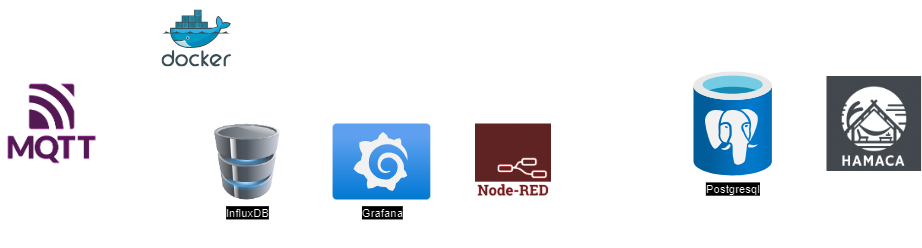
\includegraphics[scale=0.35]{./Figuras/componentes_hamaca.png}
\caption{Componentes sugeridos para la herramienta de visualización, monitoreo y control HAMACA}
\label{fig:componentes_hamaca}
\vspace*{-10pt}
\end{figure}

Finalmente con estos componentes se establecen las siguientes directrices:
\begin{itemize}

\item Se usara Mosquitto como Broker MQTT para las comunicaciones entre los dispositivos y aquel elemento que lleve la información a la base de datos. Este estará centralizado en el mismo dispositivo donde se alojará la aplicación web, aunque se recalca el hecho que pueden existir multiples brokers bajo la arquitectura de MQTT, así como también que el broker puede ser configurado de manera externa.


\item La webapp Hamaca seguirá el paradigma cliente-servidor, con un front-end marcado y distinto a su back-end. La aplicación web solo dependerá de la base de datos Postgresql para almacenar variables de configuración, estadísticas de uso y aquellas que den soporte a la autenticación y gestión de usuarios.


\item La Base de datos Influxdb solo ha de ser consultada por la integración a Grafana para la visualización y monitoreo optimo de los datos haciendo uso de los dashboards configurables dentro de la aplicación. Grafana será embebido en la aplicación web HAMACA en su frontend. Al igual forma que la implementación de MQTT este puede existir en otro punto de red pero se sugiere el despliegue en el mismo dispositivo. 

\item La herramienta de control y de gestión de flujo de tareas automatizado Node-Red, al igual que Grafana será embebida sobre el frontend de la aplicación web HAMACA. Este componente podrá interactuar también con el broker MQTT para poder transmitir (y en algunos casos, también capturar directamente) los sensores y acturadores de los prototipos de dispositivos IoT.

\end{itemize}
De esta forma se presenta el diseño de la arquitectura de la solución para el problema de investigación como se puede notar en la figura \ref{fig:arquitectura_hamaca}
\begin{figure}[!htb]
\centering
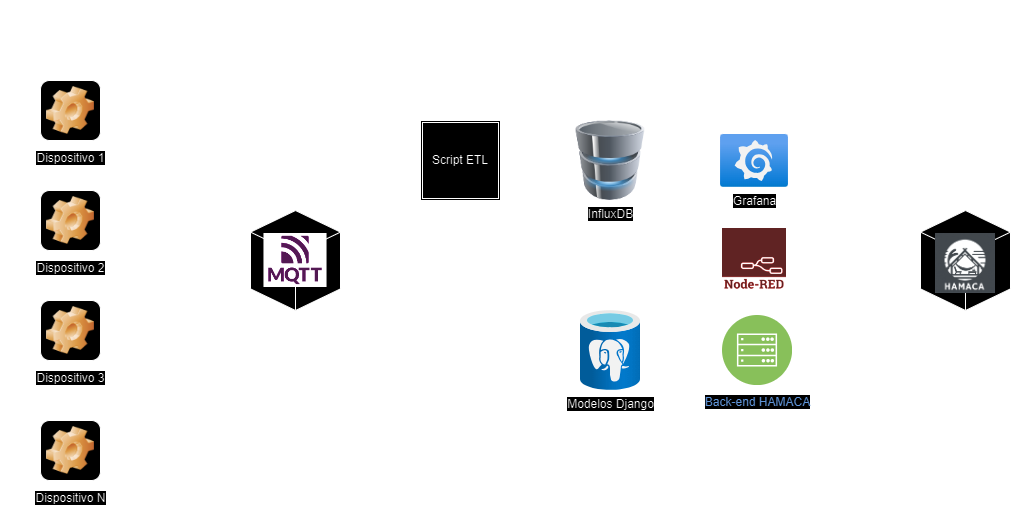
\includegraphics[scale=0.4]{./Figuras/arquitectura_hamaca.png}
\caption{Arquitectura de la solución propuesta}
\label{fig:arquitectura_hamaca}
\vspace*{-10pt}
\end{figure}

%	Sección dos: Implementación  de la solución 
\section{Implementación de la solución}
\lhead[\thepage]{\thesection. Implementación de la solución}
Siguiendo lo convenido en la sección anterior se dispuso la misma estructura organizativa de llevar por separado la implementación de los prototipos de dispositivos IoT por un lado y la aplicación web HAMACA por otro.\\

\subsection{Implementación de los prototipos de dispositivos IoT}
El proceso partió por obtener y organizar los elementos requeridos para la creación de los prototipos funcionales, es decir, las placas programables, los sensores, los actuadores, elementos de construcción de electrónicos (cables, resistencias, estaño, dispositivos de almacenamiento, protoboards, etc) y las herramientas físicas (pela cables, piqueta, soldador, tester, etc)  de manera de tener en recaudo todo lo concerniente con el desarrollo físico de los dispositivos (véase figura \ref{fig:sensores_recibidos}).
\begin{figure}[!htb]
\centering
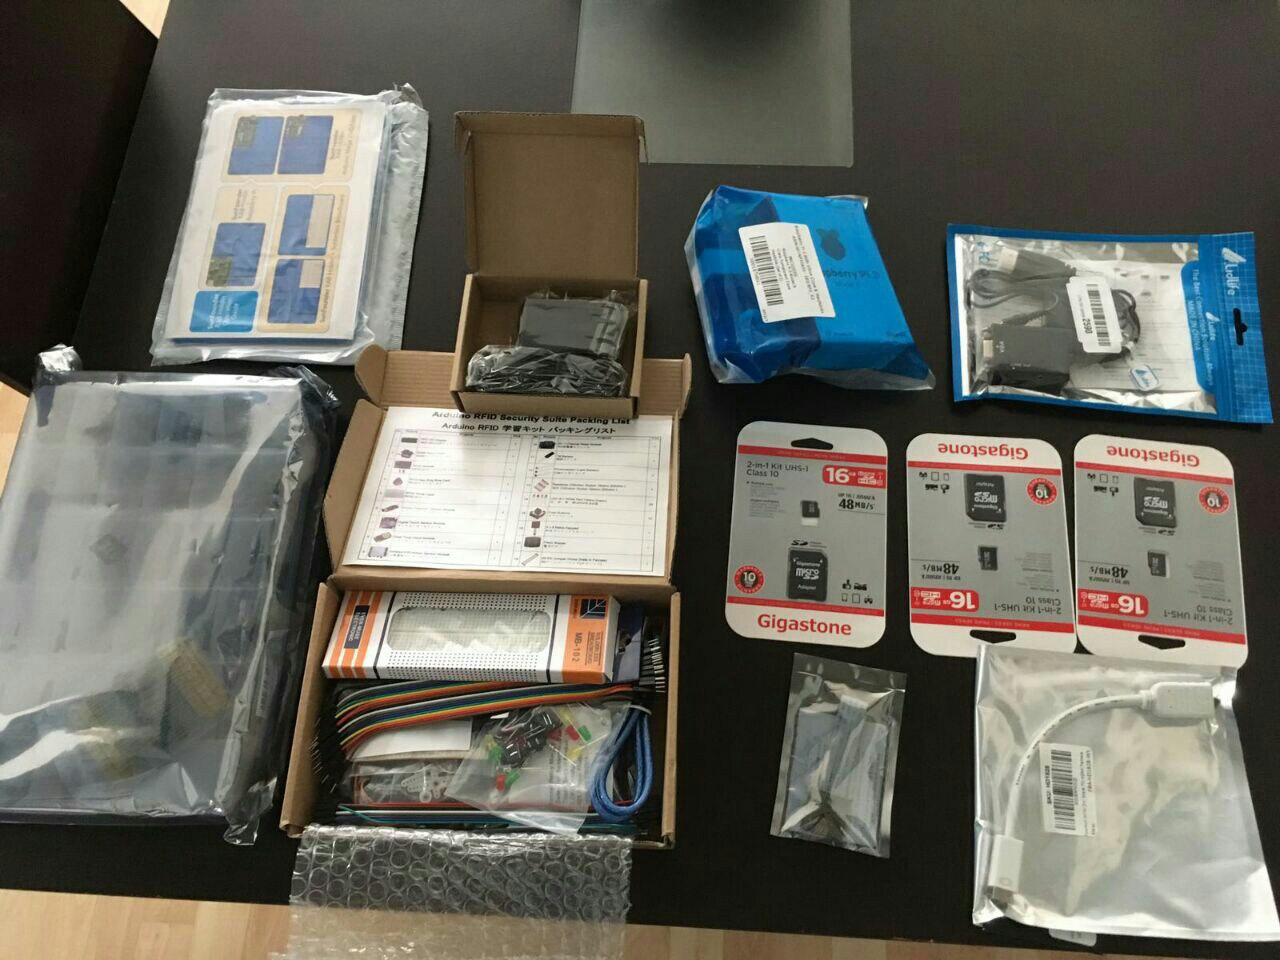
\includegraphics[scale=0.15]{./Figuras/sensores_recibidos.jpg}
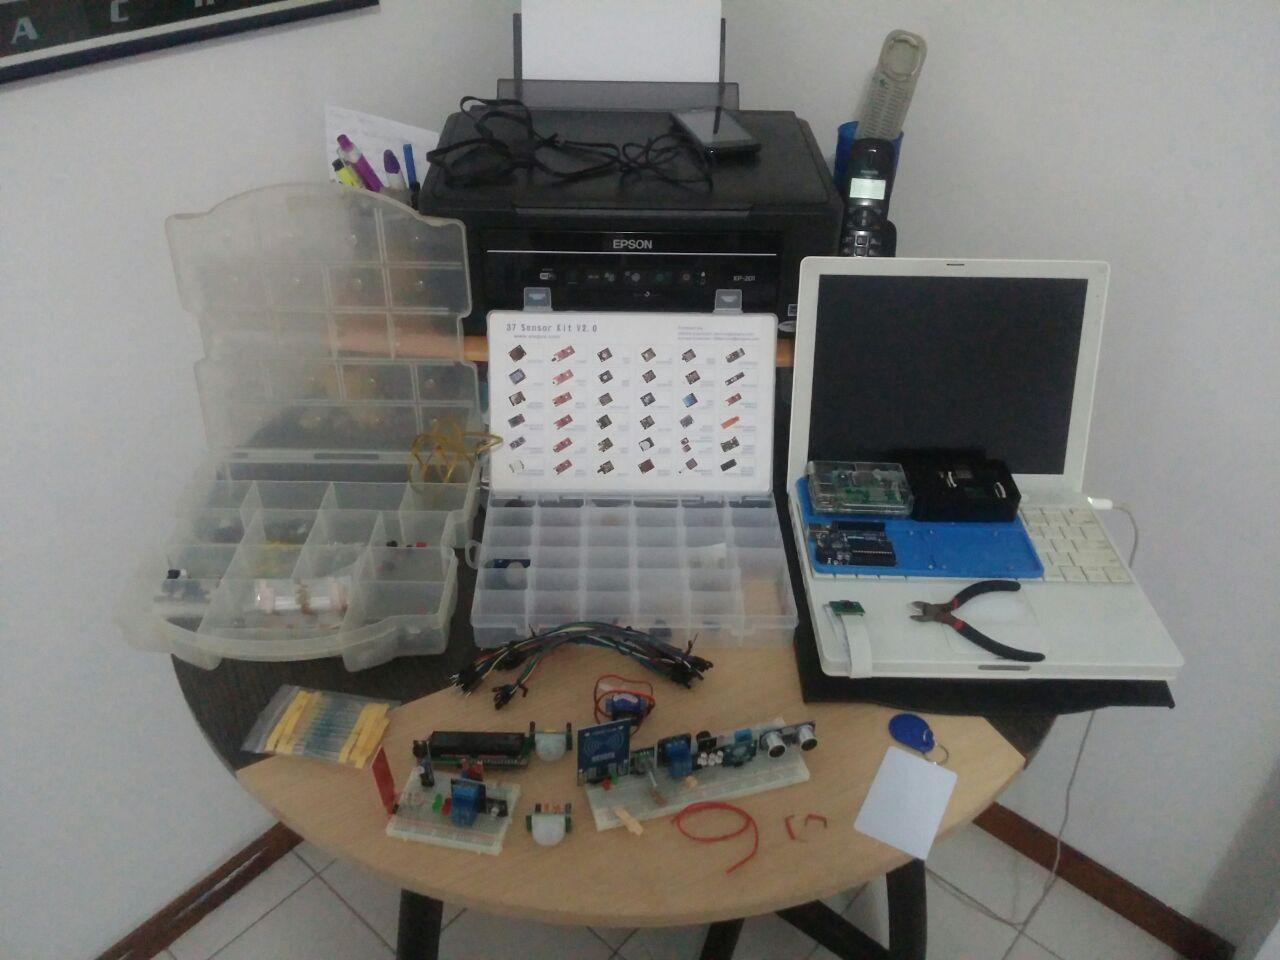
\includegraphics[scale=0.2]{./Figuras/sensores.jpg}
\caption{Elementos para prototipado de dispositivos}
\label{fig:sensores_recibidos}
\vspace*{-10pt}
\end{figure}

Una vez organizados, se construyó uno a uno cada prototipo de dispositivo, comenzando por el prototipo de dispositivo para exteriores. Tomado el arduino uno y los sensores conectados a el, junto con la computadora iBook G4 como interfaz de despliegue del código a la placa programable y para captura y envío de los datos se procedió a desarrollar dos scripts:
\begin{itemize}
\item Un primer script en el lenguaje de programación Arduino con los drivers y la lógica de control de la placa programable  para los sensores y actuadores que fueron tomados según el diseño convenido anteriormente (figuras \ref{fig:arduino_ext} y \ref{fig:sensores_ext}).
\begin{figure}[!htb]
\centering
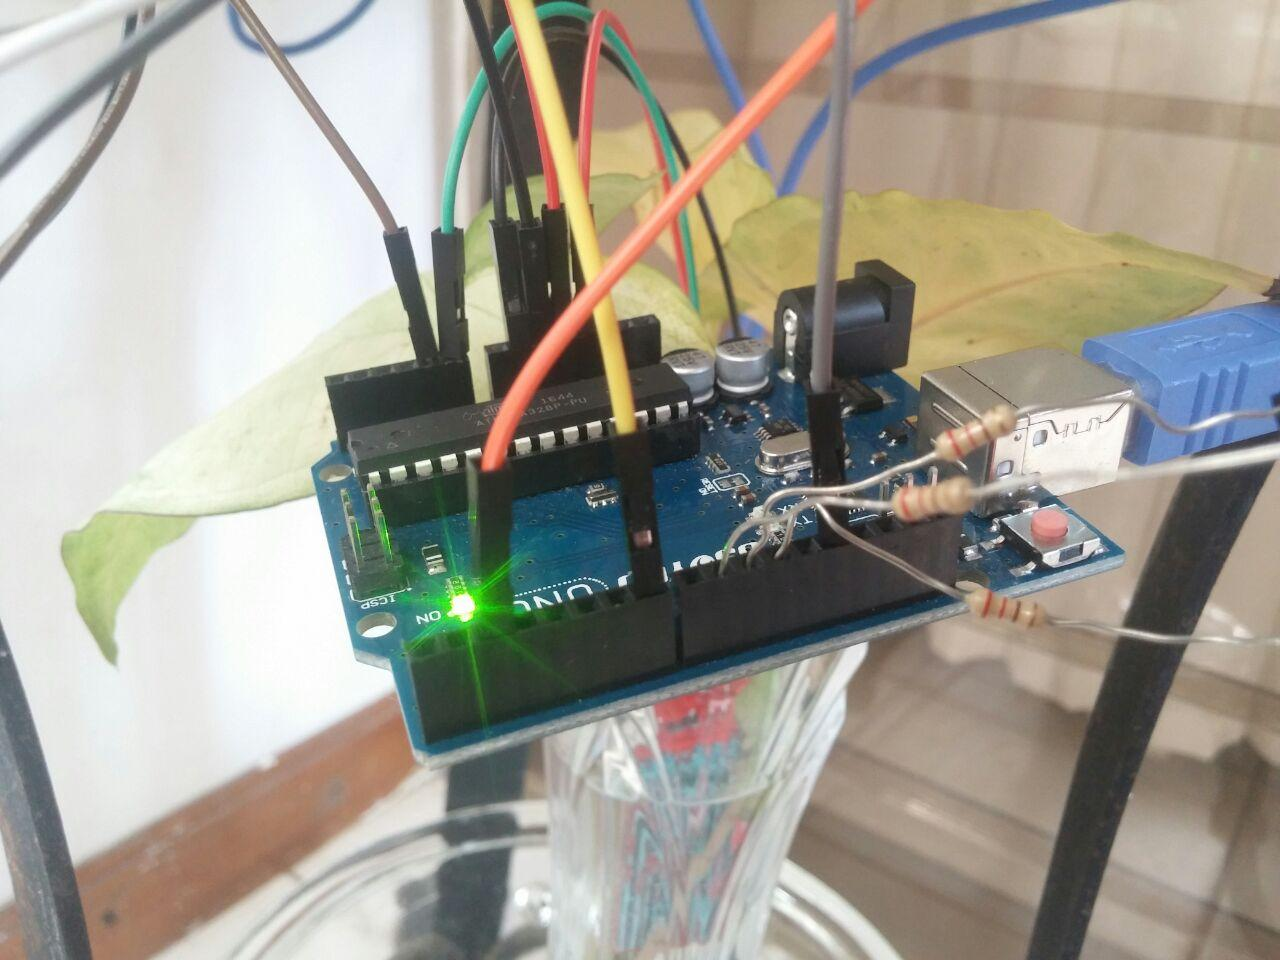
\includegraphics[scale=0.2]{./Figuras/arduino_ext.jpg}
\caption{Arduino Uno conectado a sensores y al iBook G4}
\label{fig:arduino_ext}
\vspace*{-10pt}
\end{figure}

\begin{figure}[!htb]
\centering
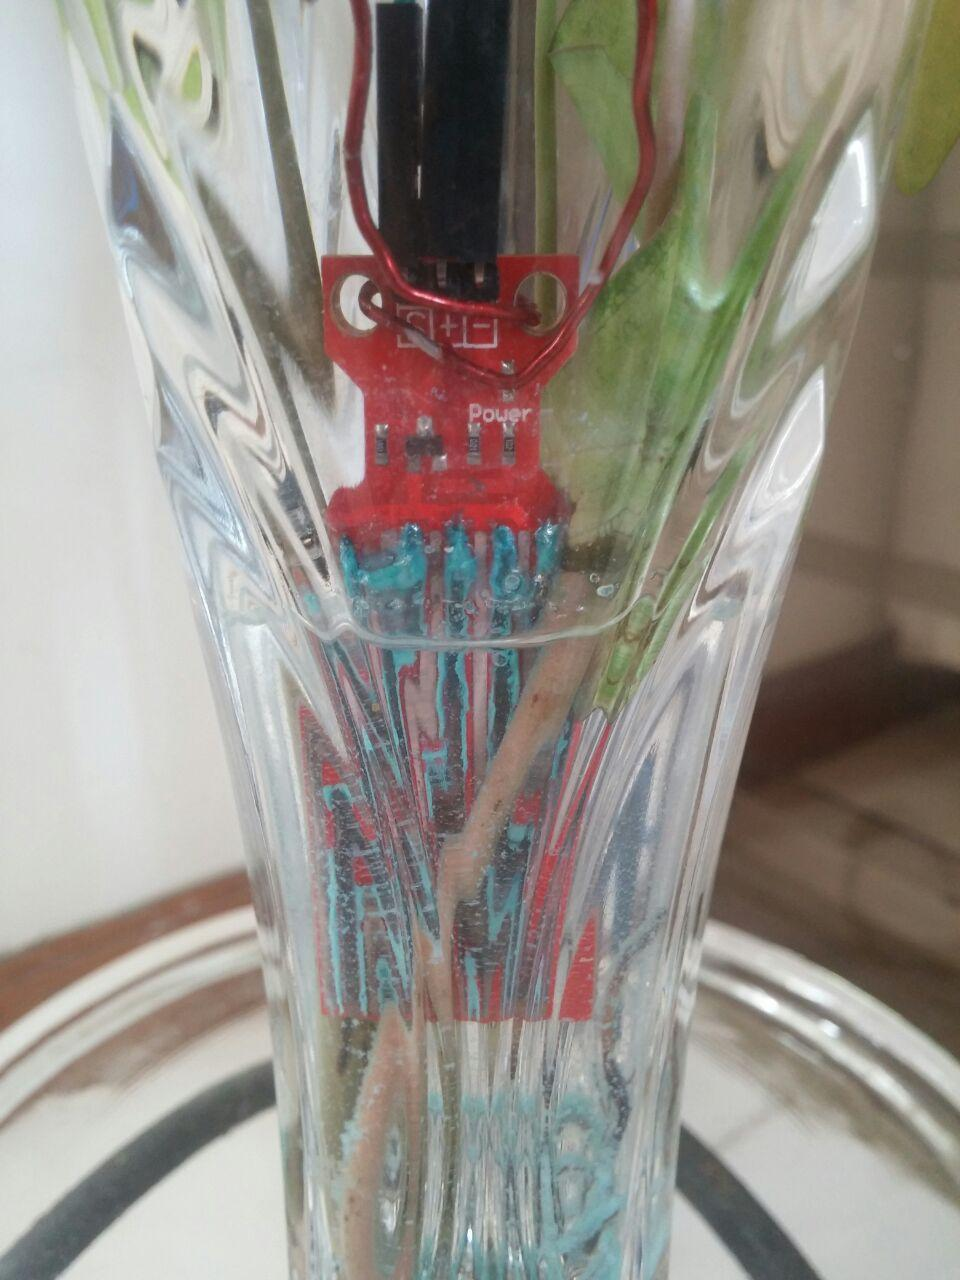
\includegraphics[scale=0.11]{./Figuras/sensor_agua.jpg}
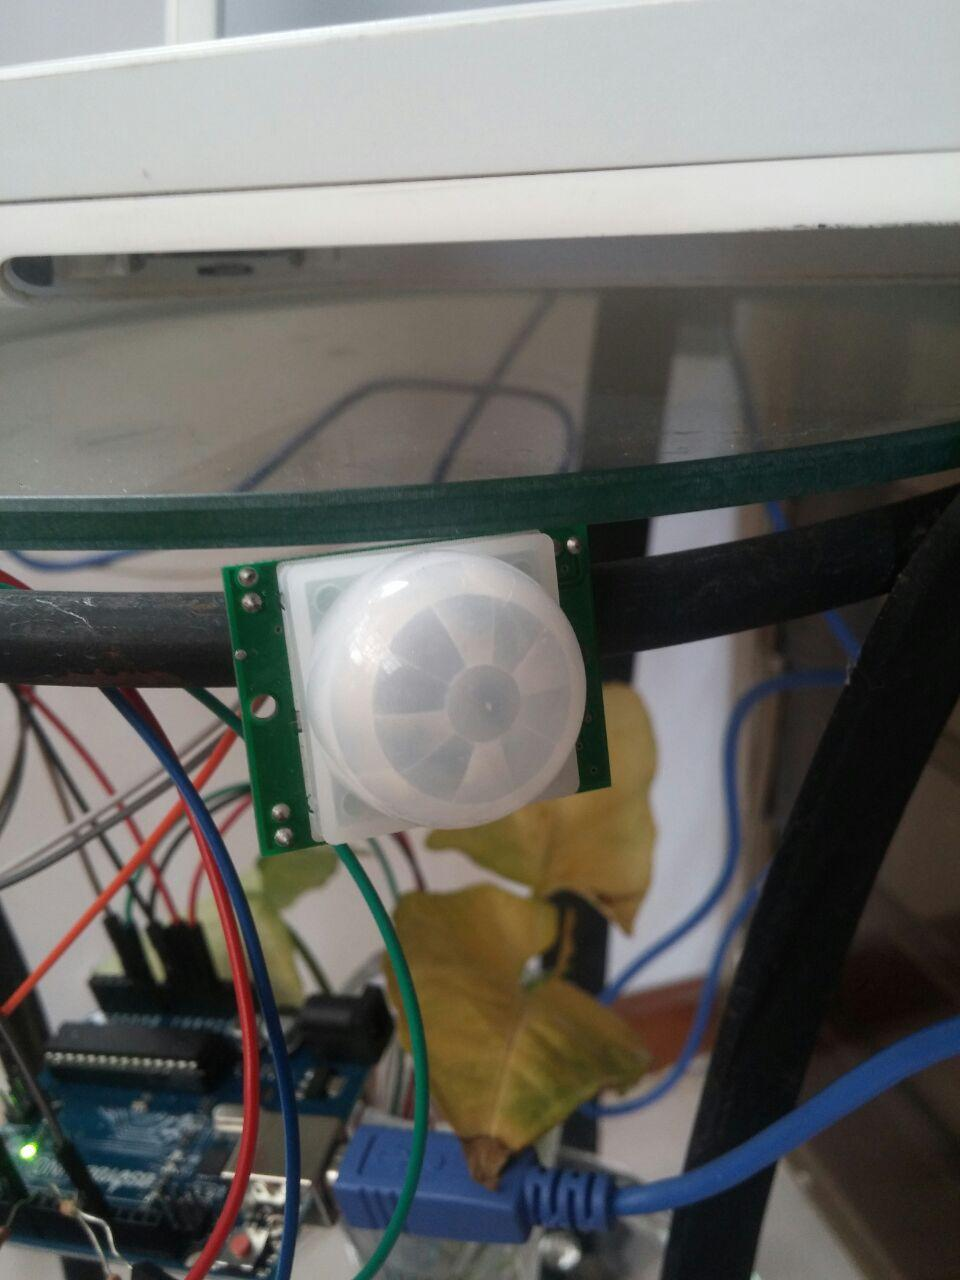
\includegraphics[scale=0.11]{./Figuras/pir_ext.jpg}
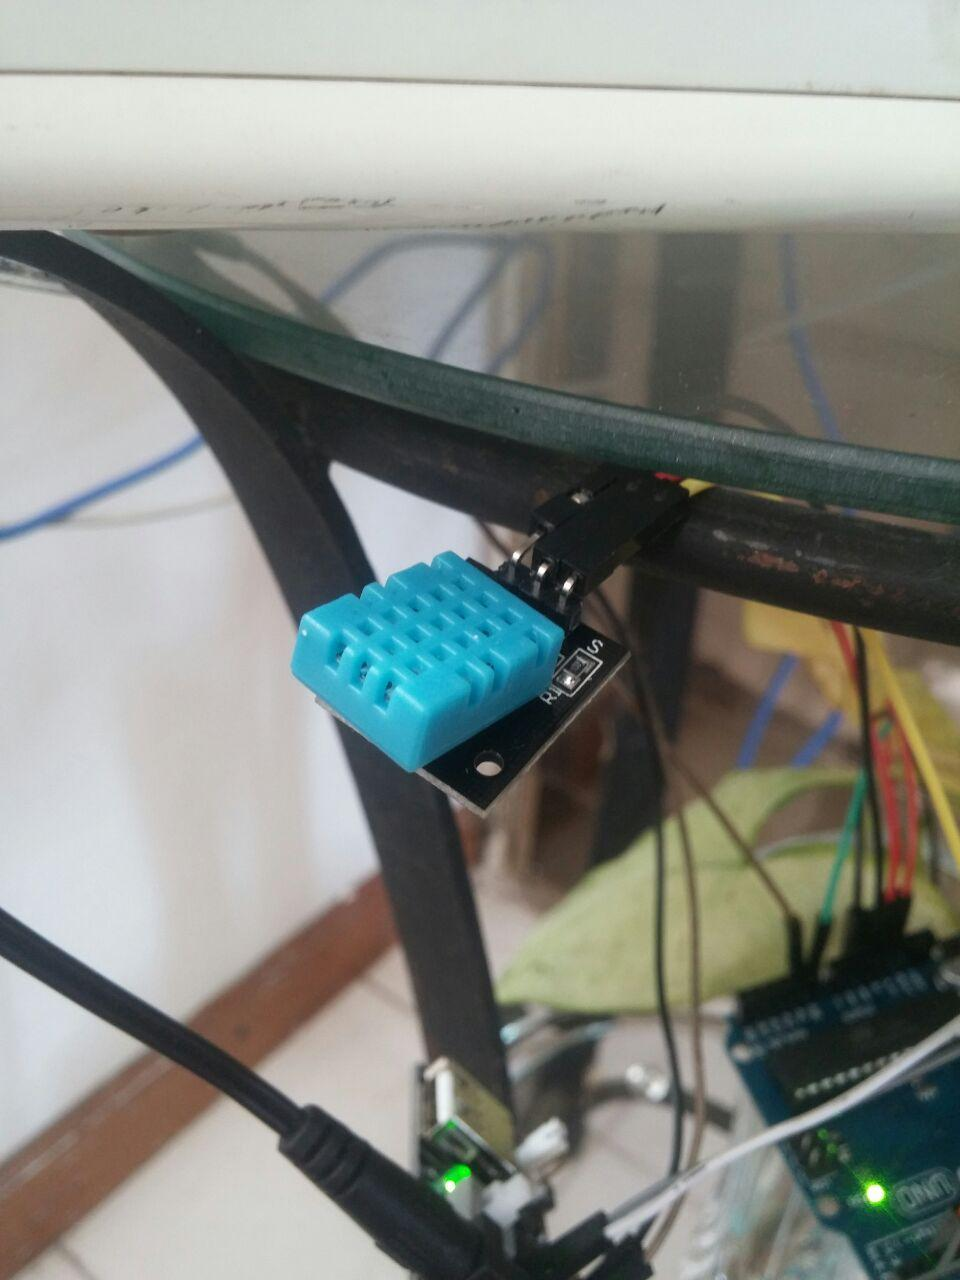
\includegraphics[scale=0.11]{./Figuras/temp_ext.jpg}
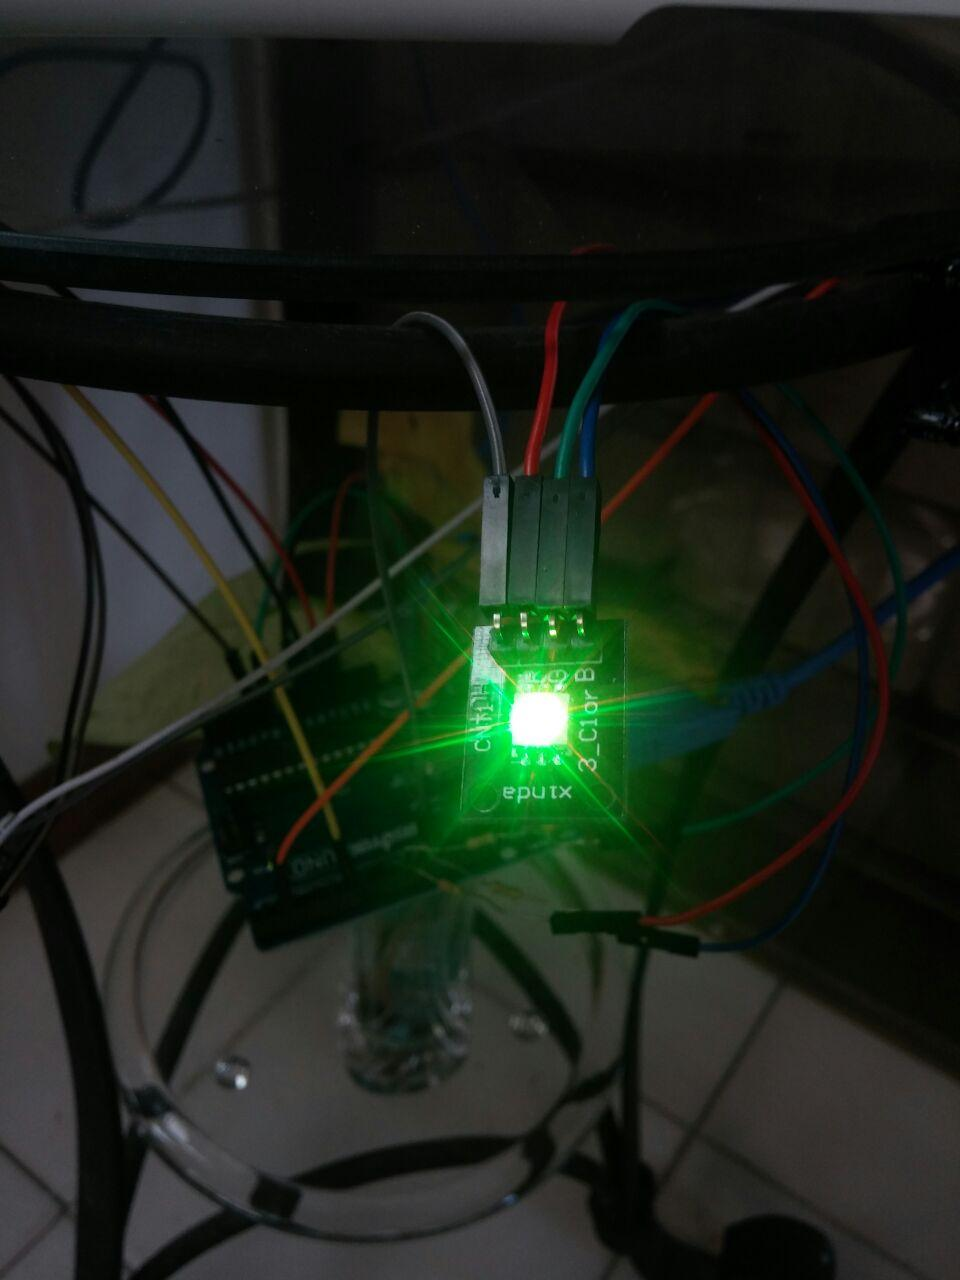
\includegraphics[scale=0.11]{./Figuras/rgb_ext.jpg}
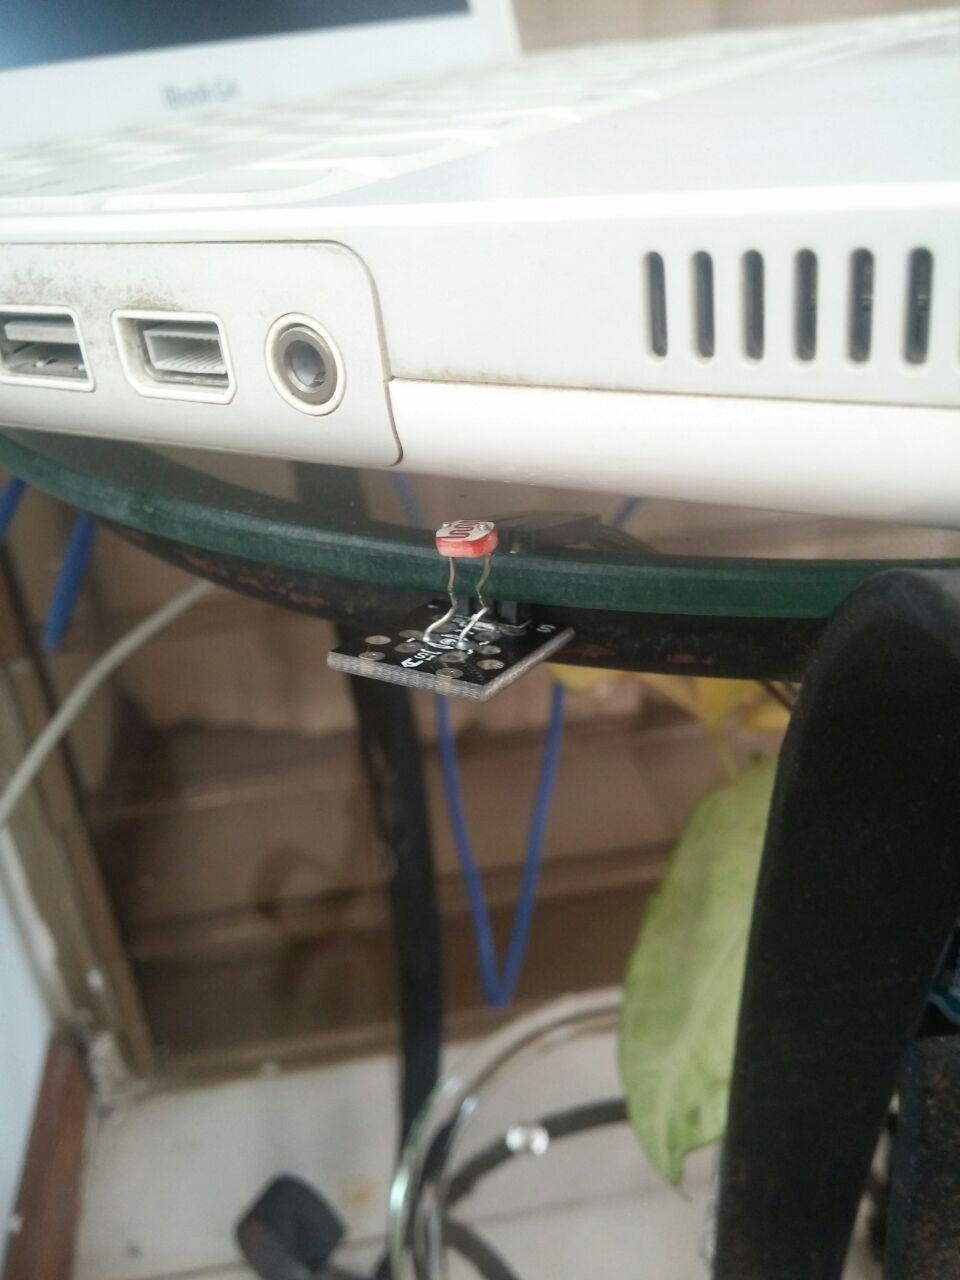
\includegraphics[scale=0.11]{./Figuras/fotorresistencia.jpg}
\caption{Sensores y actuadores en el exterior}
\label{fig:sensores_ext}
\vspace*{-10pt}
\end{figure}



\item Un segundo script en el lenguaje de programación Python con la capacidad de leer los datos seriales provenientes del Arduino Uno y con la capacidad de enviarlos a través del protocolo MQTT al broker.\ref{fig:ibook_data}  
\begin{figure}[!htb]
\centering
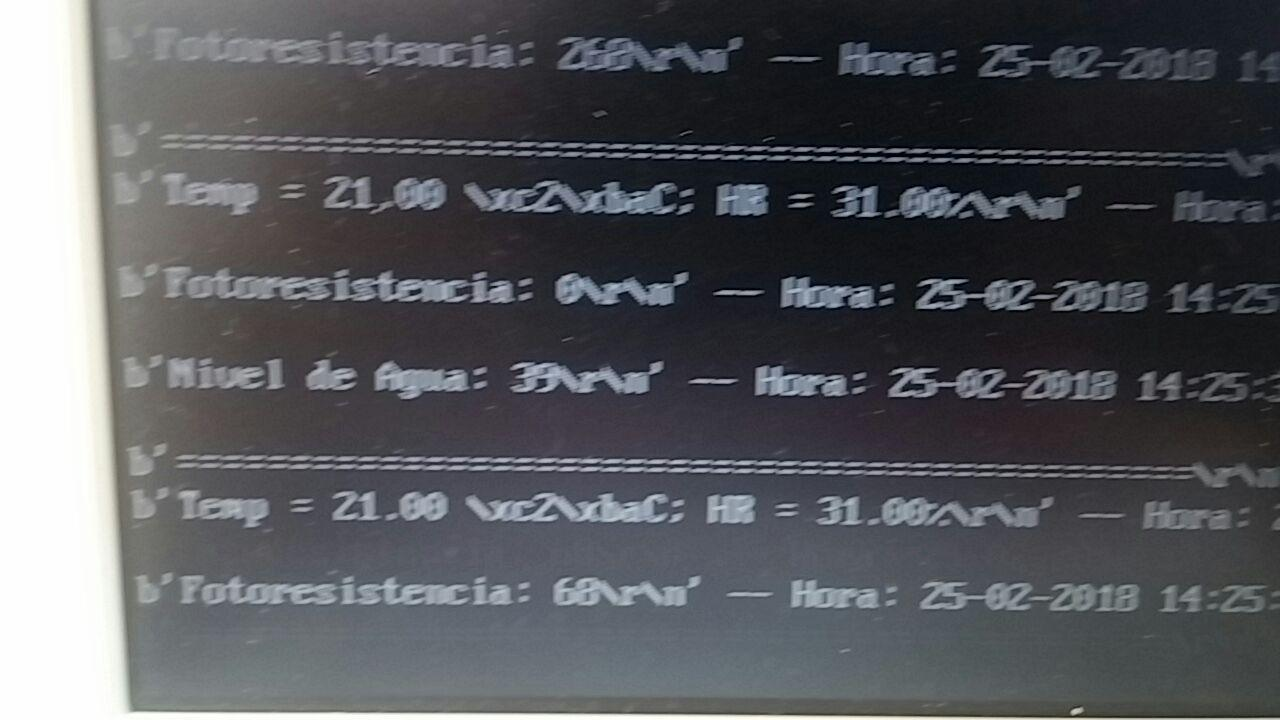
\includegraphics[scale=0.22]{./Figuras/ibook_data.jpg}
\caption{Datos siendo capturados en el Ibook G4}
\label{fig:ibook_data}
\vspace*{-10pt}
\end{figure}

\end{itemize}
Finalmente el dispositivo y el computador fueron colocados geográficamente en el balcón del apartamento para simular con la mayor precisión posible un ambiente exterior propiamente dicho.\\

El siguiente paso de manera similar consistió en construir el prototipo funcional del dispositivo IoT para ser interior del hogar. El dispositivo elegido para esta tarea fue uno de los dos Raspberry Pi 3 modelo B disponibles, así como la lista de sensores asociados para completar la tarea. De esta forma se llevaron las siguientes labores:
\begin{itemize}
\item Se realizó la colocación de todos los sensores en un protoboard y de allí fue conectados al Raspberry Pi.

\item Se instaló el sistema operativo Raspbian al dispositivo y se dejó preparado para utilizar una configuración headless, es decir, sin uso de monitor, solo acceso remoto.

\item Se desarrollaron scripts en el lenguaje de programación Python por cada sensor y actuador utilizado. 

\item una vez probado su funcionamiento se hizo un marco para poder acoplar el dispositivo y el protoboard con la ayuda de bloques de lego como se puede observar en la \ref{fig:rpi3javier_indoor}. Su disposición final geográficamente fue situado en la mitad del apartamento en la biblioteca 
\begin{figure}[!htb]
\centering
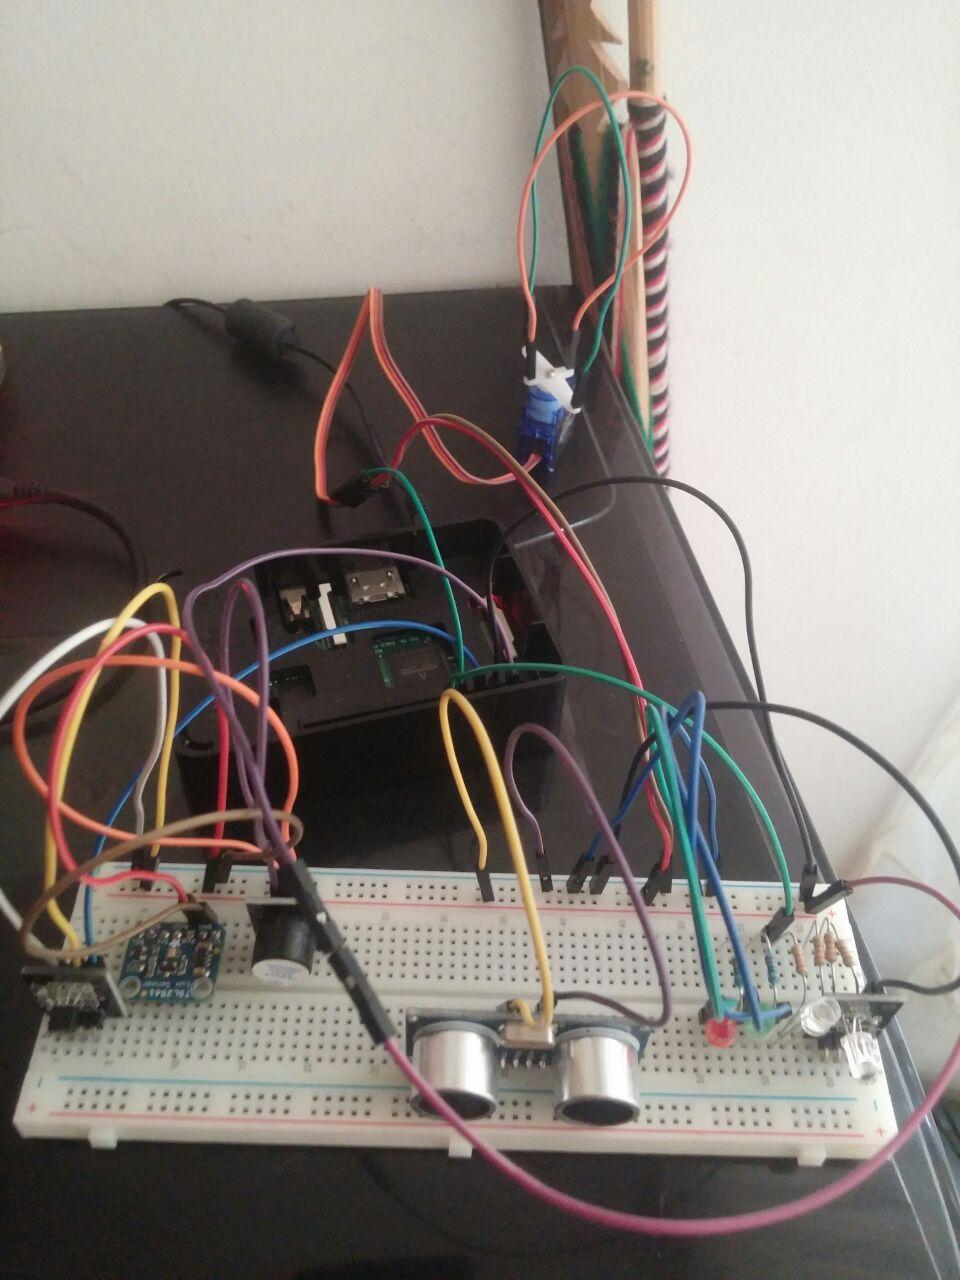
\includegraphics[scale=0.165]{./Figuras/rpi3javier_proto.jpg}
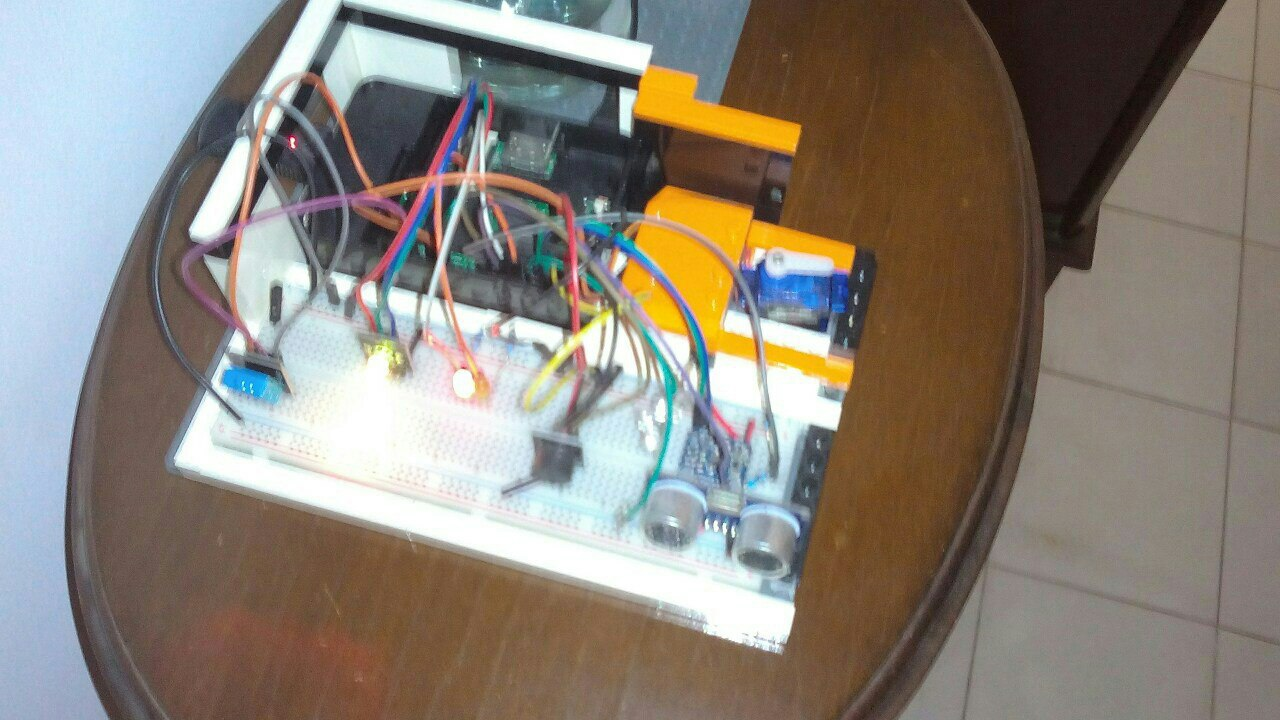
\includegraphics[scale=0.22]{./Figuras/rpi3javier_final.jpg}
\caption{Sensor IoT en el interior del hogar antes y despues de su validación}
\label{fig:rpi3javier_indoor}
\vspace*{-10pt}
\end{figure}
\end{itemize} 

Luego, se continuó con los dos prototipos que representan elementos de seguridad. Para ellos se utilizaron el Raspberry Pi Zero y el Raspberry Pi 3 modelo B restante. Para poder dejar activos los elementos correspondientes a ellos se siguieron los siguientes pasos:
\begin{itemize}
\item  Se realizó la colocación de todos los sensores y actuadores en un protoboard y de allí fue conectados al Raspberry Pi Zero.

\item Se instaló el sistema operativo Raspbian al dispositivo y se dejó preparado para utilizar una configuración headless, es decir, sin uso de monitor, solo acceso remoto.

\item Se realizó la conexión directa del Raspberry Pi Zero al Raspberry Pi 3 modelo B para proveer de conectividad a la red al dispositivo. 

\item Se desarrollaron scripts en el lenguaje de programación Python por cada sensor y actuador utilizado en Raspberry Pi zero.

\item Se desarrolló un modelo de inteligencia artificial en el lenguaje de programación Python para usar la cámara acoplada al Raspberry Pi 3 modelo B de forma que reconociera las caras de los habitantes que entrasen al hogar.  

\item Se instalaron los elementos necesarios para dar futuro soporte al despliegue de la aplicación web HAMACA en el Raspberry Pi 3 modelo B, así como también se creó un punto de acceso para los dispositivos se pudieran conectar a el de manera independiente de la red del hogar. 
\end{itemize}

Al finalizar el desarrollo del prototipo de dispositivo este fue situado validado y colocado en la entrada del hogar (figura \ref{fig:rpi3peter_zero}), cuestión que fuera centro neuralgico de los sensores de seguridad. Aparte la capacidad de computo del Raspberry Pi 3 modelo B también estaría a disposición siendo el elemento de computo definido para la siguiente etapa de la implementación.
\begin{figure}[!htb]
\centering
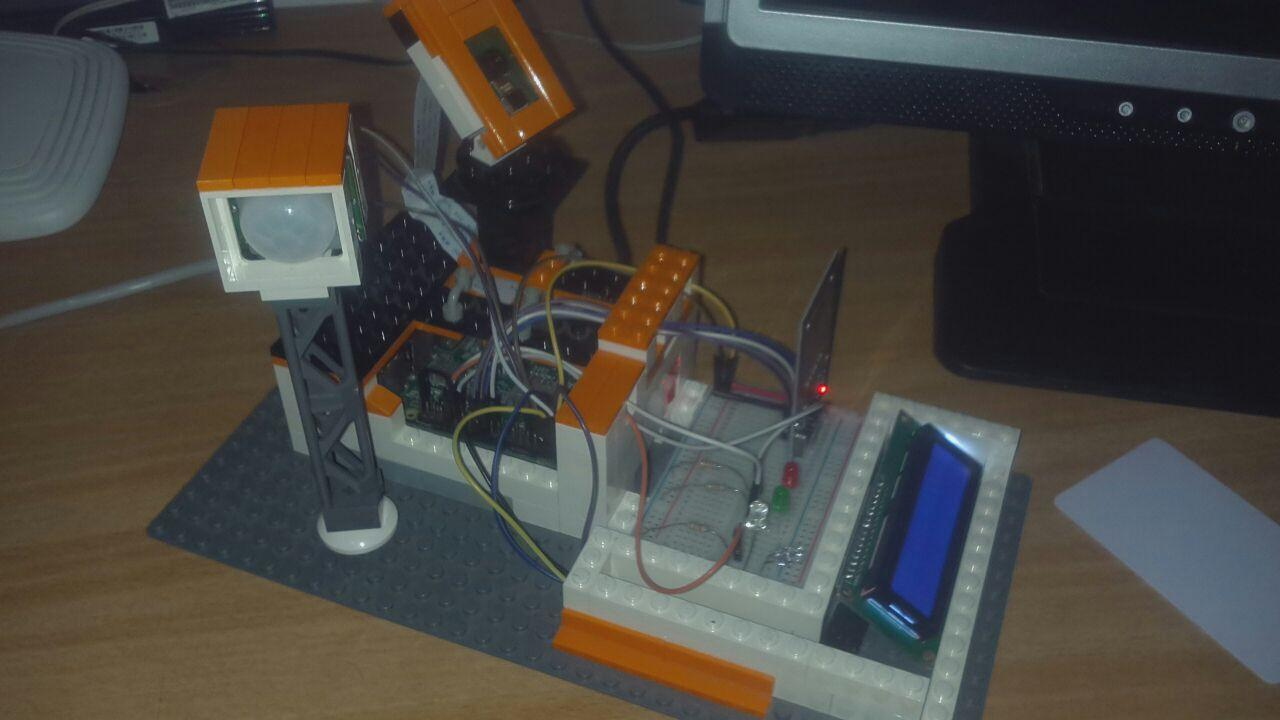
\includegraphics[scale=0.2]{./Figuras/rpi3peter_zero_proto.jpg}
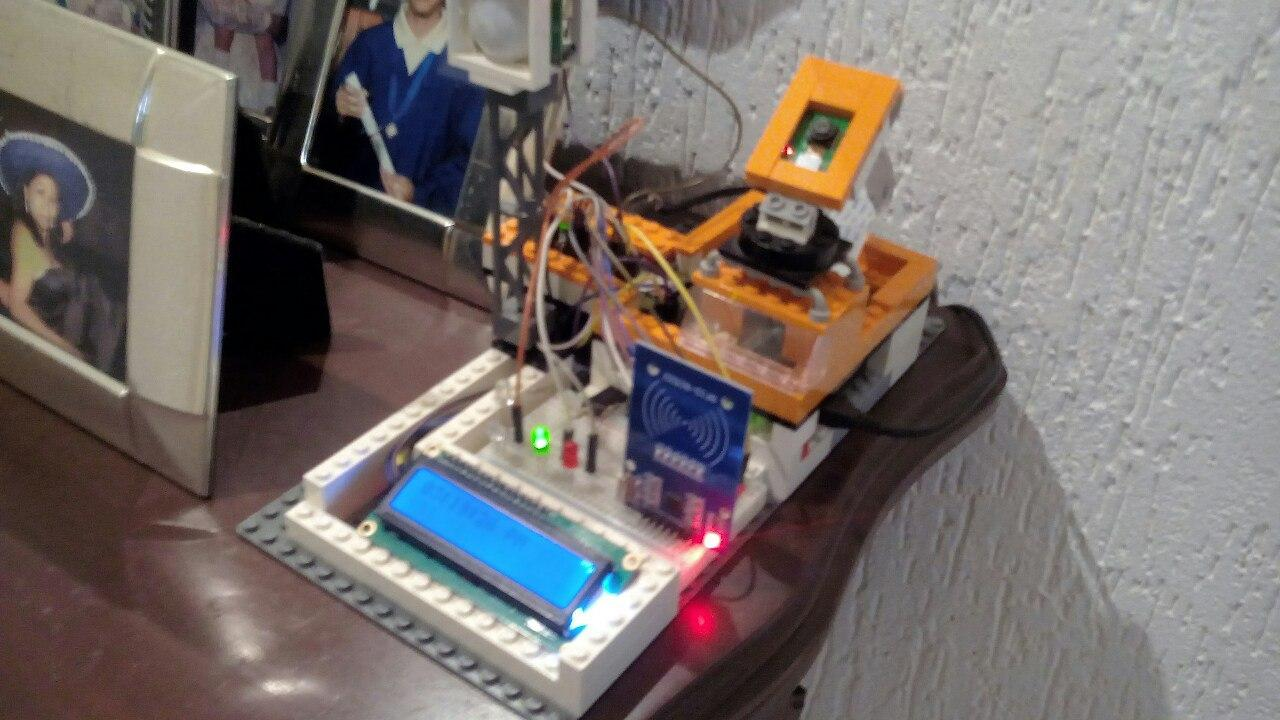
\includegraphics[scale=0.15]{./Figuras/rpi3peter_zero.jpg}
\caption{Sensor IoT en el interior del hogar antes y despues de su validación}
\label{fig:rpi3peter_zero}
\vspace*{-10pt}
\end{figure}


\subsection{Implementación de la Aplicación Web HAMACA}
Por el lado de la aplicación web HAMACA, el proceso de implementación fue llevado a cabo siguiendo los lineamientos de las metodologías ágiles, con entregables incrementales, rápidas iteraciones con nuevas características y corrección de errores. Se estimó inicialmente un período de desarrollo de aproximadamente un mes y medio para tener todos los aspectos necesarios para cubrir los objetivos planteados y dar una propuesta de solución al problema de investigación.

Los pasos que se siguieron para poder desarrollar y desplegar la webapp fueron los siguientes:

\subsubsection{Infraestructura}
Por el lado de la infraestructura, al tener como elemento de computo para despliegue un Raspberry Pi 3 Modelo B, el sistema operativo base utilizado fue raspbian, un flavor de Debian, una opción popular y fácil de utilizar para los desarrollos de software.\\

Directamente sobre el sistema operativo se instalaron todos y cada uno de los paquetes, base de datos (InfluxDB y Postgresql), herramientas a integrar (Grafana y Node-Red), la implementación de MQTT, así como también el ambiente de Python 3 para manejar la webapp.  Este proceso cambió para luego dejar la mayor cantidad de elementos posibles para ser utilizados bajo el esquema de contenedores docker, siendo migrados a esa forma la base de datos InfluxDB, y las herramientas Grafana y Node-Red. Lo cual permite un despliegue mucho más rápido en cualquier ambiente nuevo, así como modularizar el proyecto de una mejor forma.

\subsubsection{Configuración de Entorno}
Una vez instalados los diversos paquetes y herramientas se procedió con la configuración de todos los elementos previos a la parte de desarrollo.
\begin{itemize}
\item La configuración asociada a la comunicación entre los dispositivos basados en el broker MQTT instalado. 
\item La creación de una base de datos en InfluxDB, junto con un usuario y métodos de acceso de forma de almacenar a través del backend de la aplicación toda la data relativa a los dispositivos. 
\item Despliegue de la herramienta de visualización y monitoreo Grafana. Configuraciones asociadas para la conexión a la fuente de datos (base de datos InfluxDB) así como también el acceso y privilegios de gestión de cuadros de mando sin la necesidad de un usuario logeado y con privilegios asociados.
\item Despliegue de la herramienta Node-Red para el control de dispositivos. Se le armó configuraciones para poder crear interfaces basadas en cuadros de mando para poder realizar tareas de control sobre sensores y actuadores de los dispositivos. También se probaron y validaron la posibilidad de generar flujos de tareas para los dispositivos a través de esta herramienta.
\end{itemize}

\subsubsection{Desarrollo de la Aplicación Web HAMACA}
Finalmente con el entorno configurado se procede a comenzar el desarrollo de la aplicación web HAMACA (siglas de ``Herramienta de Automatización, Monitoreo y Análisis de Componentes y Artefactos"). Fue diseñada como una webapp liviana y sencilla haciendo uso del framework Django para el lenguaje de programación Pyhon en su versión 3.\\

Al comenzar el proyecto se creó la aplicación a partir de la plantilla de instrucciones que provee el framework, junto con la definición de utilizar Postgresql como base datos, puesto que es una respuesta más robusta que SQLite (base de datos por defecto) tanto para el soporte mismo de la aplicación como de sus futuros procesos. Es así como luego de configurada la base y siguiendo las instrucciones se genero en la base de datos de HAMACA los modelos que podemos observar en la figura \ref{fig:django_schema}.
\begin{figure}[!htb]
\centering
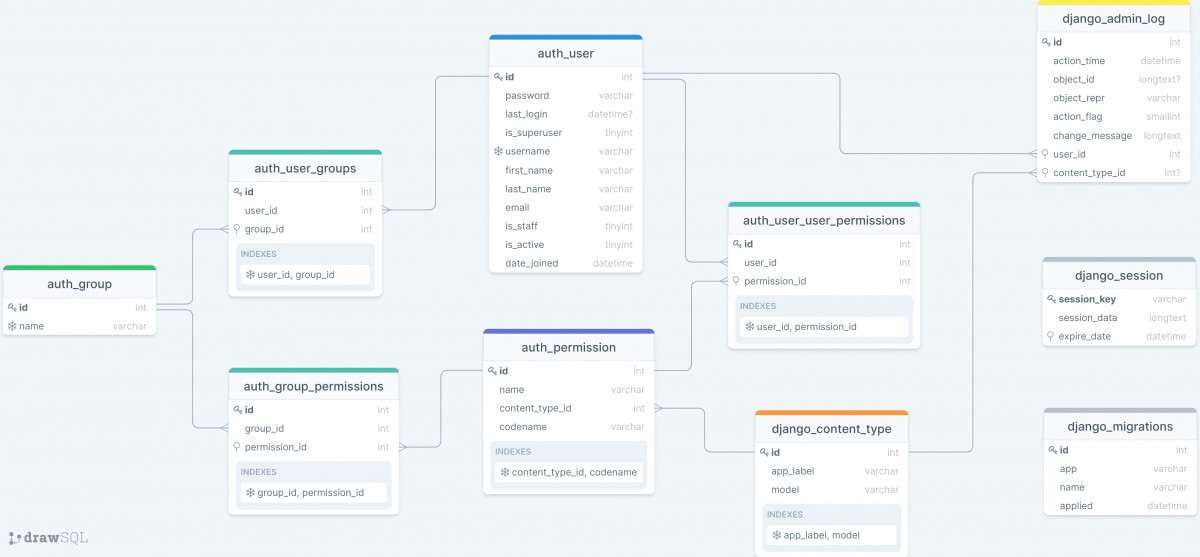
\includegraphics[scale=0.28]{./Figuras/django_schema.jpg}
\caption{Modelo autogenerado por el framework Django}
\label{fig:django_schema}
\vspace*{-10pt}
\end{figure}

En el argot de Django, este primer paso se le llama migración. Con ello se comienzo con el desarollo del primer modulo de control y acceso a la aplicación basado en los aspectos de roles y privilegios del que se dispone en el framework. También se estructuran las bases para un desarrollo modular en el que se fueron integrando progresiva e incrimentalmente nuevos elementos entre los cuales se encuentran las librerías comunes, templates para los aspectos visuales, los elementos estáticos como las fuentes para los textos, gráficos, colores, etc.\\

El primer modulo desarrollado fue el de acceso a la aplicación (figura \ref{fig:login_ui}) y el de configuraciones (figura \ref{fig:hamaca_config}), el cual contiene las herramientas de gestión de la aplicación, como la administración de usuarios, así como la capacidad de cambar la ubicación de las herramientas integradas, sea que se encuentren de manera local o en algún lugar que pueda ser accedido por este desarrollo.\\
\begin{figure}[!htb]
\centering
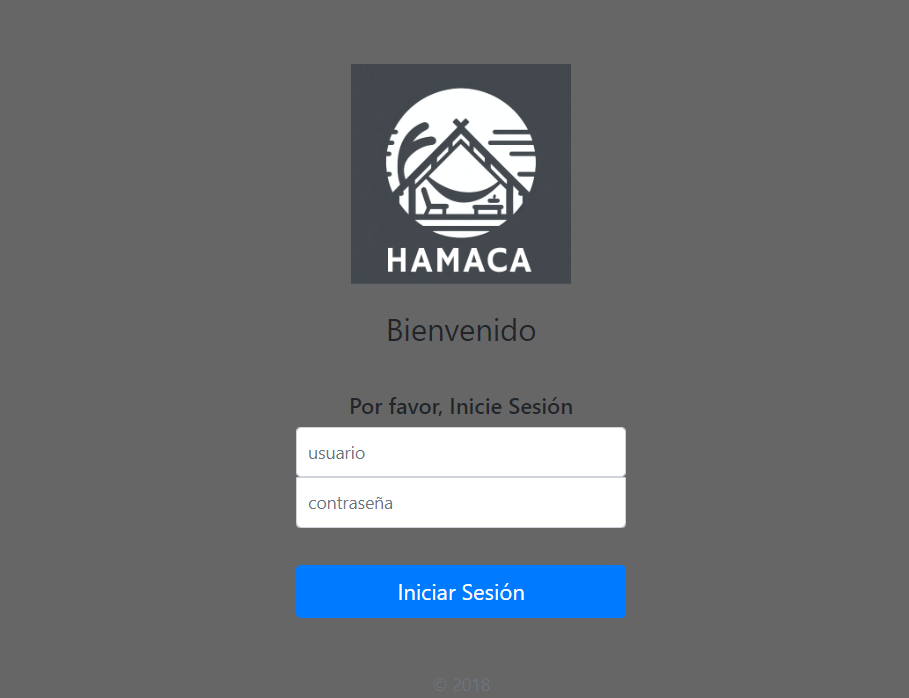
\includegraphics[scale=0.285]{./Figuras/login_ui.png}
\caption{Interfaz de inicio de sesión para los usuarios}
\label{fig:login_ui}
\vspace*{-10pt}
\end{figure}

\begin{figure}[!htb]
\centering
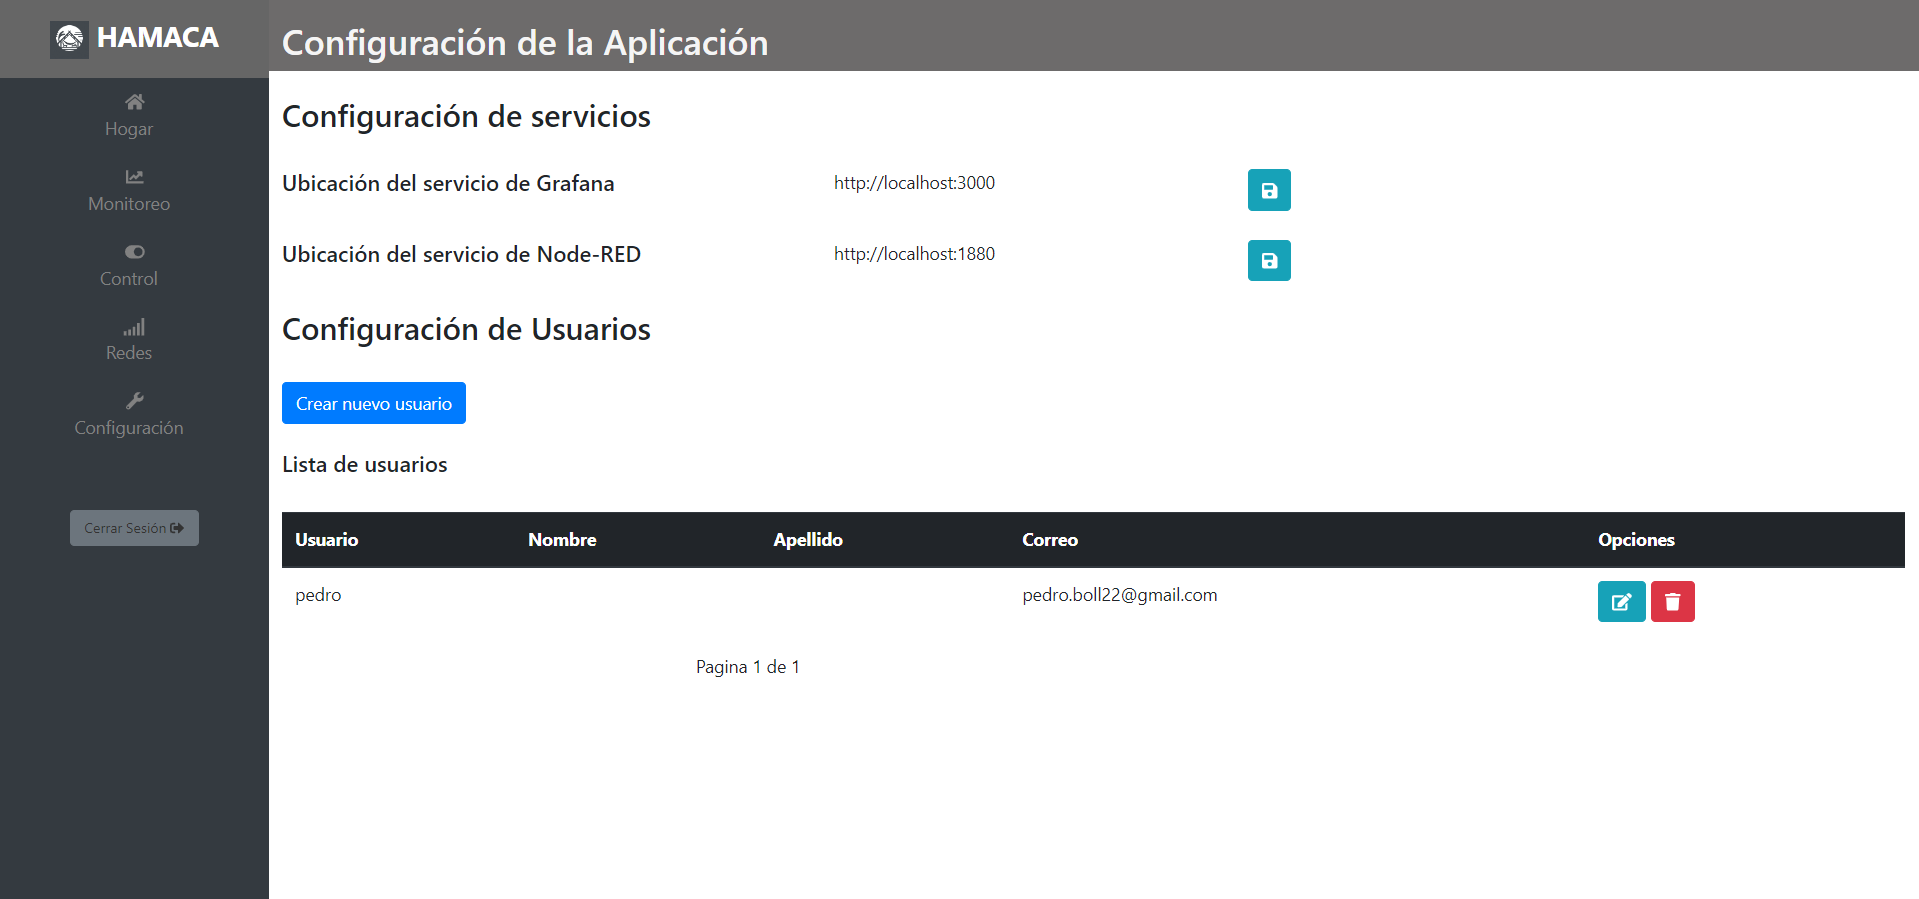
\includegraphics[scale=0.21]{./Figuras/hamaca_config.png}
\caption{Interfaz de configuración de la aplicación}
\label{fig:hamaca_config}
\vspace*{-10pt}
\end{figure}

A partir del punto anterior se creó un modulo de Monitoreo el cual contiene la lógica para integrar de manera adecuada la herramienta Grafana para visualización y monitoreo de datos, de forma que los usuarios puedan crear sus cuadros de mando de una manera sencilla y directa (figura \ref{fig:hamaca_grafana}).\\
\begin{figure}[!htb]
\centering
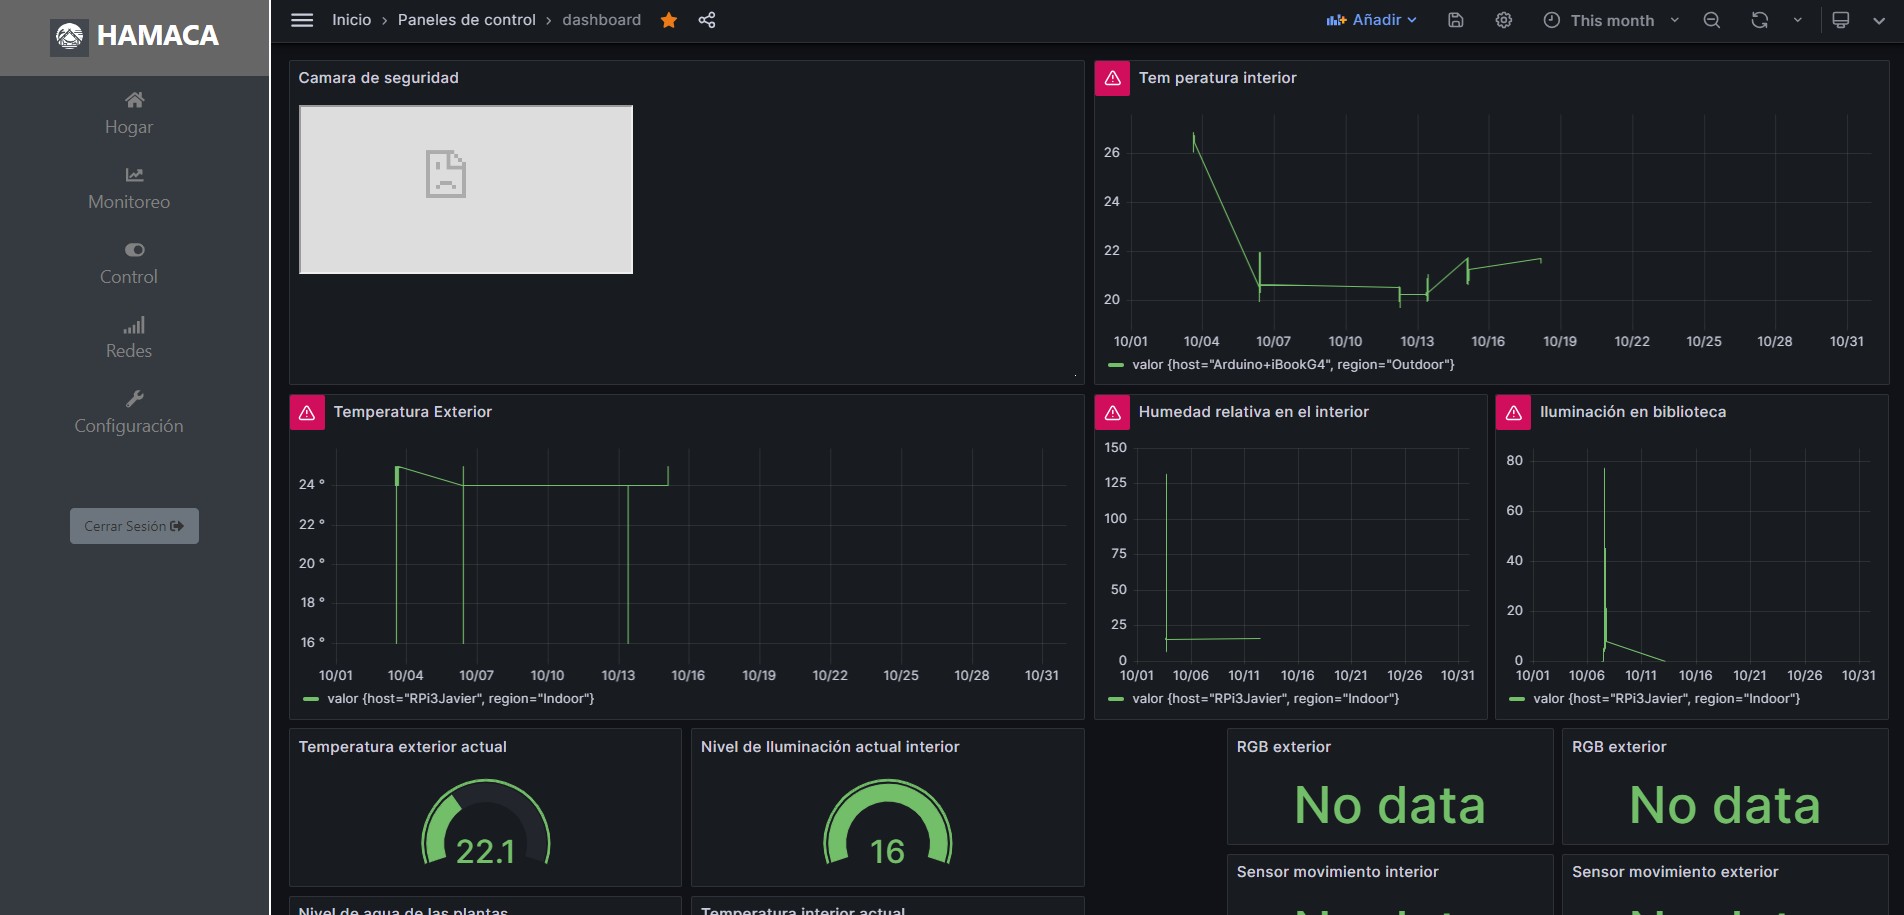
\includegraphics[scale=0.21]{./Figuras/hamaca_grafana.png}
\caption{Interfaz de visualización de datos con la herramienta Grafana embebida}
\label{fig:hamaca_grafana}
\vspace*{-10pt}
\end{figure}

De manera análoga se creó un modulo de control y un home que contienen la lógica de la integración de la herramienta Node-Red para llevar a cabo las labores de controlar y gestionar flujos de trabajo complejos con los dispositivos (figura \ref{fig:hamaca_nodered}). El home de la aplicación particularmente se convierte en un punto donde se muestran los cuadros de mando creados para manipular (e incluso observar) sensores y actuadores de aquellos dispositivos que registremos en los flujos para mostrar (figura \ref{fig:hamaca_home}).\\

\begin{figure}[!htb]
\centering
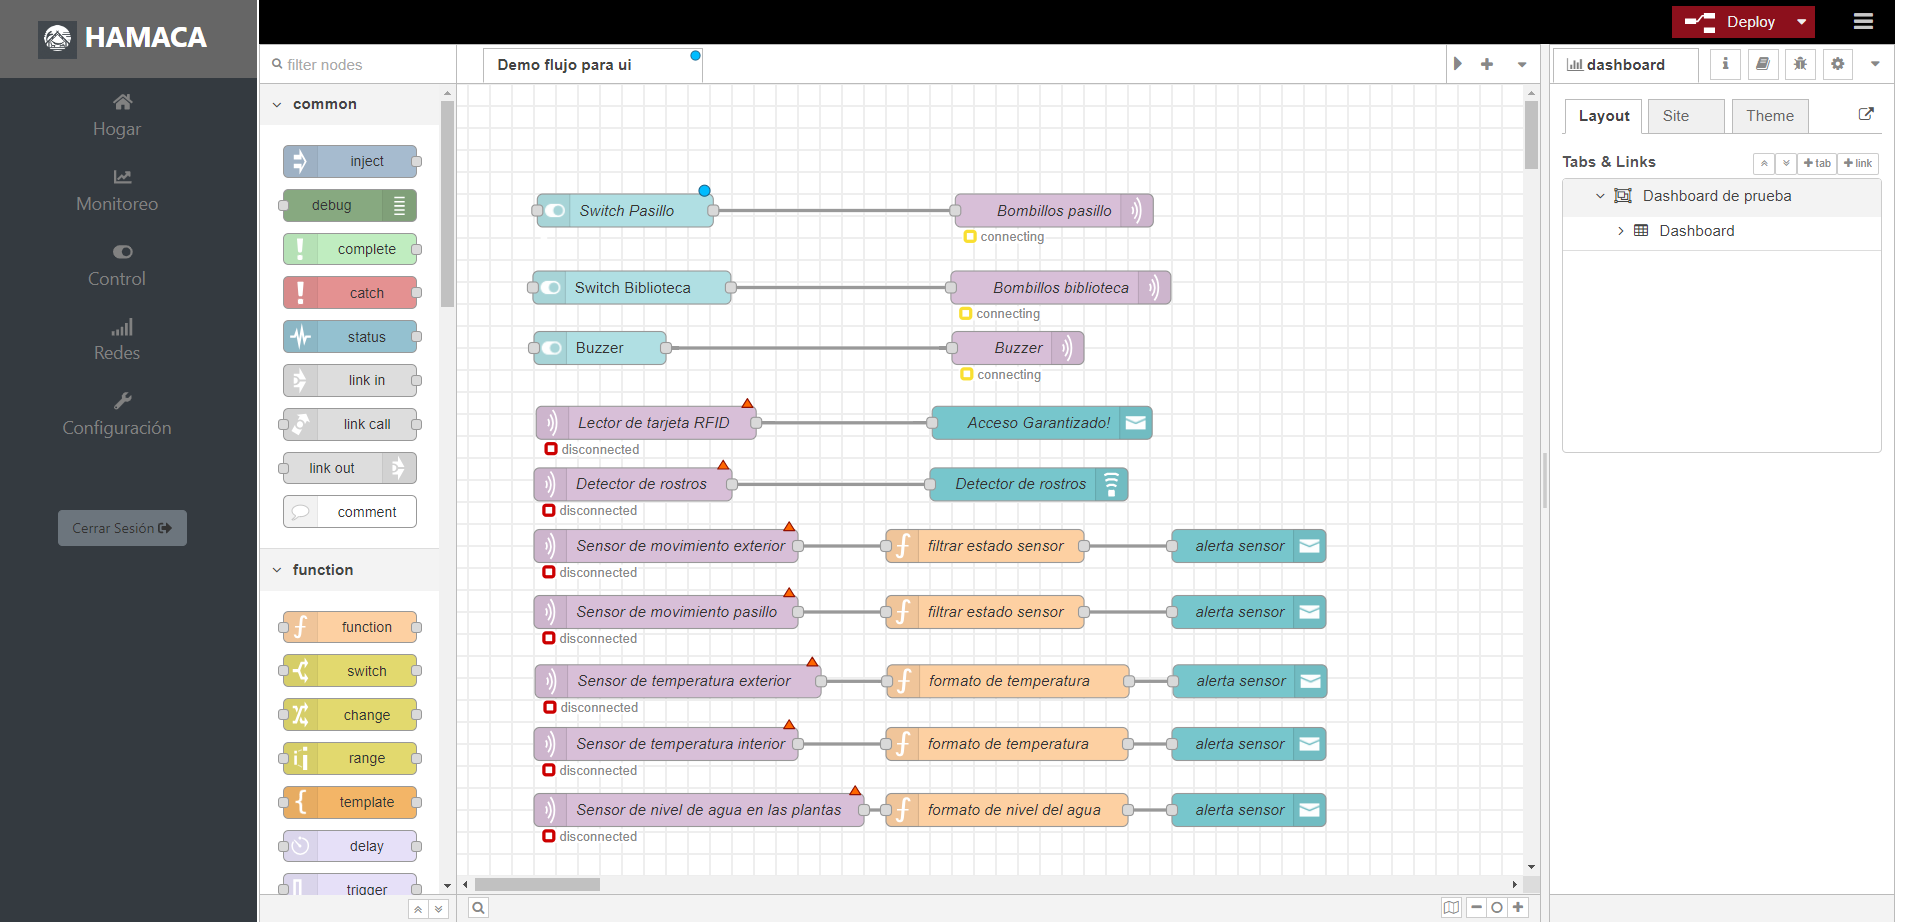
\includegraphics[scale=0.21]{./Figuras/hamaca_nodered.png}
\caption{Interfaz de flujos de automatización con la herramienta Node-Red embebida}
\label{fig:hamaca_nodered}
\vspace*{-10pt}
\end{figure}

\begin{figure}[!htb]
\centering
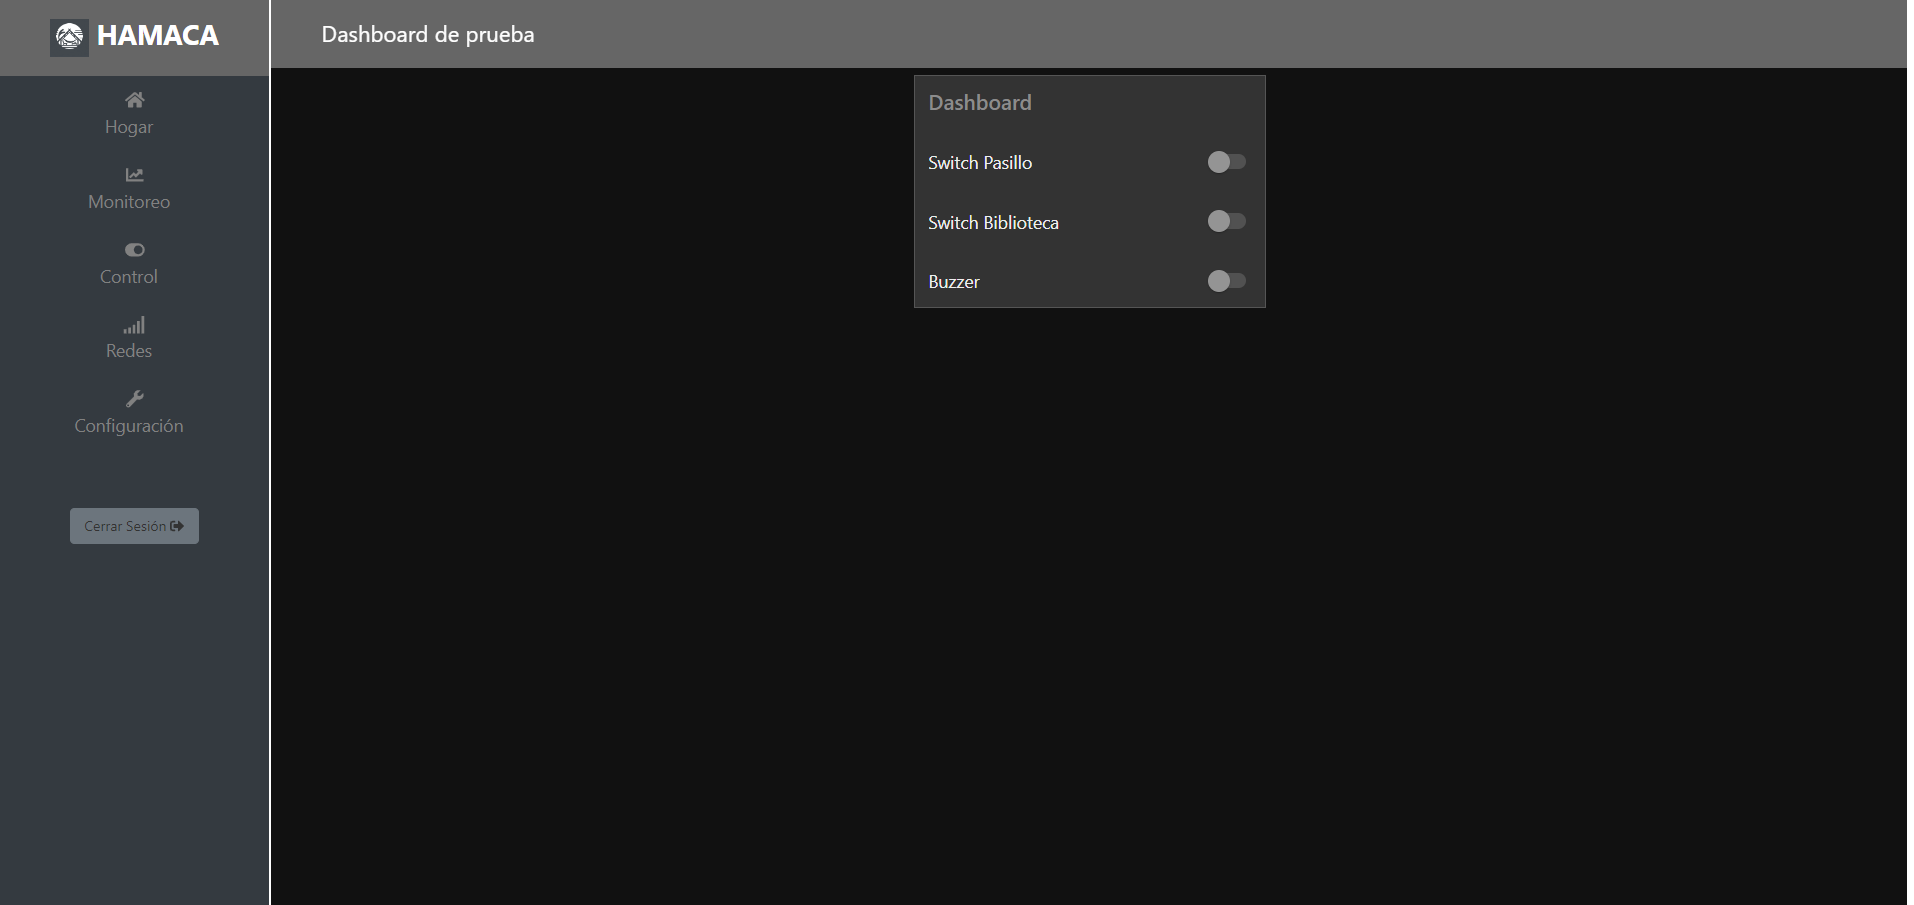
\includegraphics[scale=0.2]{./Figuras/hamaca_home.png}
\caption{Interfaz de control de dispositivos a través del dashboard de Node-Red}
\label{fig:hamaca_home}
\vspace*{-10pt}
\end{figure}

Por último pero no menos importante se creó un apartado de redes en el cual se pueden observar los registros de las comunicaciones realizadas entre los dispositivos y el broker, así como otras métricas asociadas a ello (figura \ref{fig:hamaca_redes}).

\begin{figure}[!htb]
\centering
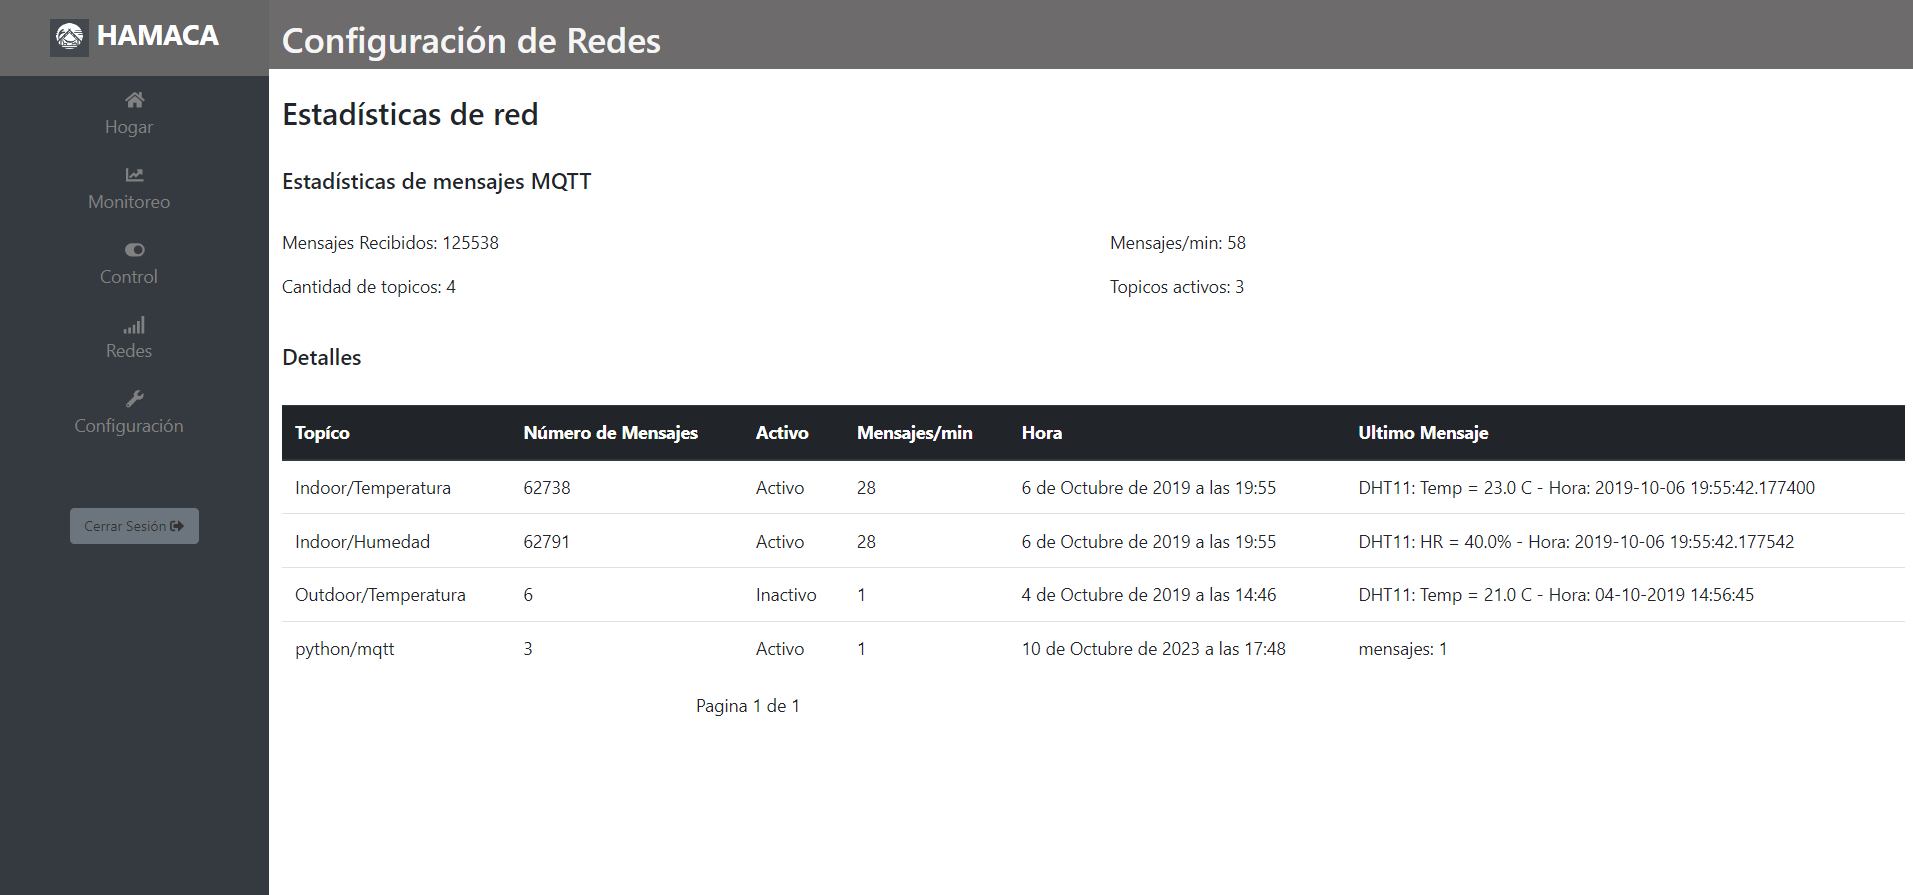
\includegraphics[scale=0.2]{./Figuras/hamaca_redes.png}
\caption{Interfaz de la aplicación para la configuración y visualización de métricas de red}
\label{fig:hamaca_redes}
\vspace*{-10pt}
\end{figure}

Luego del desarrollo de cada modulo y aunque no todos los módulos interactuan con la base de datos se realizó nuevamente el proceso de migración, de forma que la base de datos se adaptara a los requerimientos nuevos de los módulos existentes. Así la base de datos se le agregaron dos nuevas tablas como se pueden observar en la figura \ref{fig:psql_hamaca_db}
\begin{figure}[!htb]
\centering
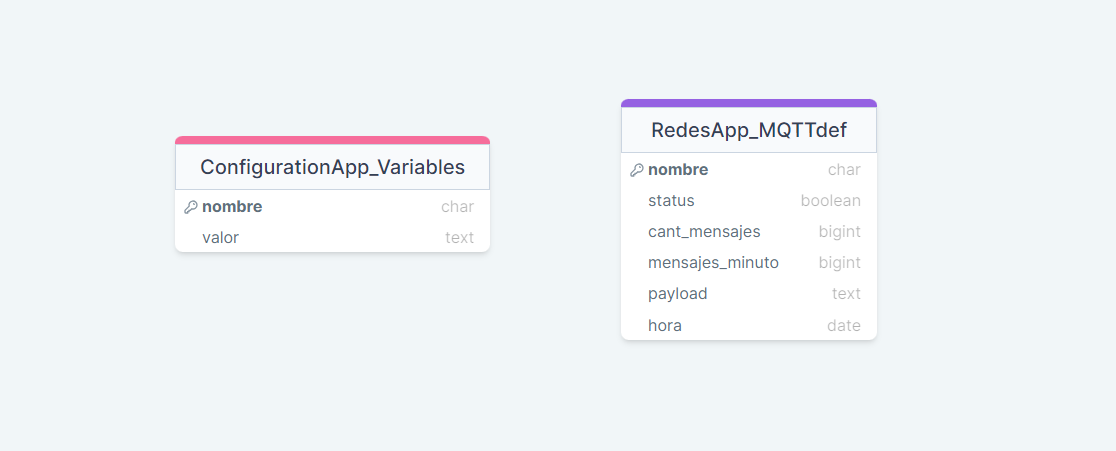
\includegraphics[scale=0.19]{./Figuras/psql_hamaca_db.png}
\caption{Modelo de la base de datos HAMACA}
\label{fig:psql_hamaca_db}
\vspace*{-10pt}
\end{figure}

% Capitulo siete
%-----------------------------------------------------------------------------
%	 Entorno de Pruebas
%-----------------------------------------------------------------------------

\lhead[\thepage]{ Entorno de Pruebas \thechapter. \rightmark}
\rhead[ Entorno de Pruebas \thechapter. \leftmark]{\thepage}

%	Capitulo N:  Entorno de Pruebas
\chapter{ Entorno de Pruebas}
\markboth{ Entorno de Pruebas}{ Entorno de Pruebas}
hue
\section{Escenarios de pruebas}
hue

%	Capitulo ocho
%-----------------------------------------------------------------------------
%	 Casos de Uso 
%-----------------------------------------------------------------------------

\lhead[\thepage]{Casos de Uso \thechapter. \rightmark}
\rhead[Casos de Uso \thechapter. \leftmark]{\thepage}

%	Capitulo 8: Casos de Uso
\chapter{Casos de Uso}
\markboth{Casos de Uso}{Casos de Uso}
Para la solución prevista, especificamente los componentes de que requieren comunicarse usando MQTT como protocolo se establece el caso de uso :

\begin{figure}[htb]
\centering
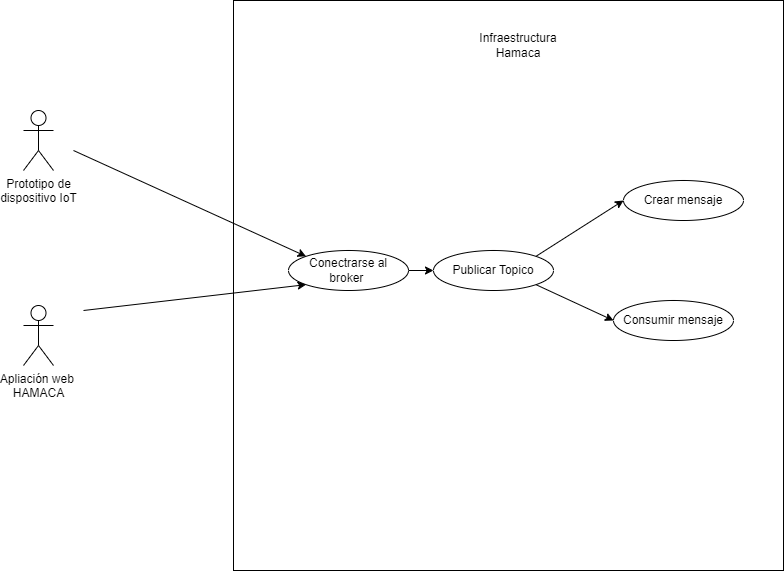
\includegraphics[scale=0.35]{./Figuras/caso_de_uso_mqtt.png}
\caption{Diagrama de caso de uso para la comuniación MQTT}
\label{fig:caso_de_uso_mqtt}
\vspace*{-10pt}
\end{figure}

A continuación se explica cada acción dentreo del caso de uso:
\begin{itemize}
\item el tal
\end{itemize}

\begin{figure}[htb]
\centering
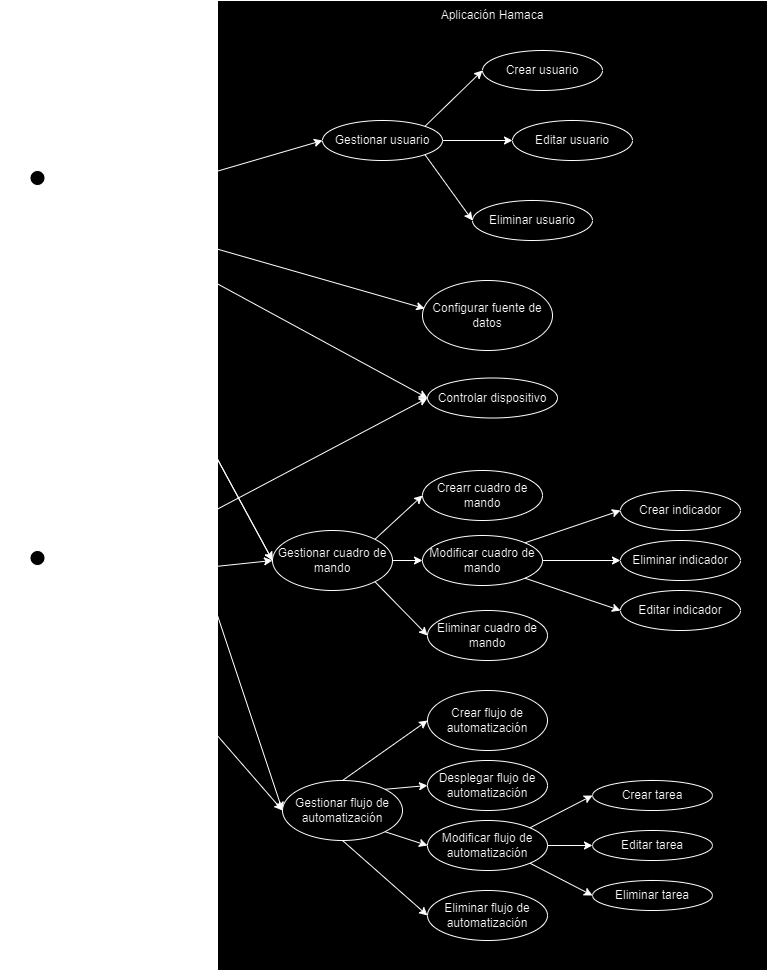
\includegraphics[scale=0.35]{./Figuras/caso_de_uso.png}
\caption{Diagrama de caso de uso para la apliación web HAMACA}
\label{fig:caso_de_uso}
\vspace*{-10pt}
\end{figure}


\section{Laboratorios de Investigación y Desarrollo}
\lhead[\thepage]{\thesection. Laboratorios de Investigación y Desarrollo}
hue
\subsection{Entornos Académicos}
hue
\subsection{Entornos Industriales}
hue

\section{Ambientes Domésticos y Oficinas}
\lhead[\thepage]{\thesection. Ambientes Domésticos y Oficinas}
hue

%	Capitulo nueve
%-----------------------------------------------------------------------------
%	 Resultados, Limitaciones y Trabajos Futuros
%-----------------------------------------------------------------------------

\lhead[\thepage]{Resultados, Limitaciones y Trabajos Futuros \thechapter. \rightmark}
\rhead[Resultados, Limitaciones y Trabajos Futuros \thechapter. \leftmark]{\thepage}

%	Capitulo N: Conclusiones
\chapter{Resultados, Limitaciones y Trabajos Futuros}
\markboth{Resultados, Limitaciones y Trabajos Futuros}{Resultados, Limitaciones y Trabajos Futuros}
hue
\section{Resultados}
hue
\section{Limitaciones}
hue
\section{Contribuciones}
hue
\section{Trabajos Futuros}
hue
%	Capitulo diez
%-----------------------------------------------------------------------------
%	 Conclusiones
%-----------------------------------------------------------------------------

\lhead[\thepage]{Conclusiones \thechapter. \rightmark}
\rhead[Conclusiones \thechapter. \leftmark]{\thepage}

%	Capitulo N: Conclusiones
\chapter{Conclusiones}
\markboth{Conclusiones}{Conclusiones}

Este trabajo de investigación permitió demostrar la factibilidad del desarrollo de una herramienta de visualización de datos, monitoreo, control y automatización de procesos concernientes a dispositivos de Internet de las cosas, partiendo desde prototipos funcionales que pudiesen generar información para llevarlo a un escenario lo más realista posible sobre el como de desplegaría un futuro contexto donde los artefactos inteligentes son ubicuos.\\

El desarrollo de prototipos de dispositivos IoT permitió identificar las fortalezas y debilidades de los enfoques utilizados para medir y controlar estos artefactos de manera transparente. Se observaron como el fenómeno de la variedad entre sensores, actuadores y dispositivos en si pueden generar data que aunque representen lo mismo tiene matices de eficiencia y eficacia que pueden ser aprovechados por otros elementos en la búsqueda de capturar, mostrar y utilizar la información que capturamos de ellos.\\

Por el lado del desarrollo de la aplicación web se demostró que un software que pueda orquestar e integrar herramientas existentes para tareas especificas como visualización de datos, automatización de procesos, monitoreo y control de dispositivos puede ser una alternativa viable para poder centralizar las operaciones inherentes a dispositivos IoT y que es un esquema flexible que permite no solo adaptarse a las necesidades de los usuarios sino también con alta capacidad de crecimiento futuro, sea desde el punto de vista de protocolos y estándares, como de software análisis automatizado.\\

Finalmente, se considera que los objetivos planteados en el marco del planteamiento del problema fueron cumplidos con éxito y se espera que este software sea al final de utilidad en donde el contexto permita aprovechar las funcionalidades desarrolladas anteriormente, sea dentro del ámbito académico, investigativo, industrial o uso personal.


%	Referencias bibliográfica
\lhead[\thepage]{BIBLIOGRAFÍA}
\bibliography{Referencias/Referencias}
\end{document}
